% Generated fragments require trusted human review before compilation.
% This binder never requests shell escape or runs external tools.
\documentclass[11pt]{article}
% Trusted shared apparatus. Requires LuaLaTeX; never use shell escape.
\usepackage{fontspec}
\defaultfontfeatures{Ligatures=TeX}
\IfFontExistsTF{Noto Serif}{\setmainfont{Noto Serif}}{%
  \IfFontExistsTF{DejaVu Serif}{\setmainfont{DejaVu Serif}}{%
    \IfFontExistsTF{Times New Roman}{\setmainfont{Times New Roman}}{%
      \PackageError{gelfand-binder}{No configured Cyrillic serif font installed}{Install Noto Serif or DejaVu Serif, or select an installed Cyrillic font.}%
    }%
  }%
}
\IfFontExistsTF{Noto Sans}{\setsansfont{Noto Sans}}{%
  \IfFontExistsTF{DejaVu Sans}{\setsansfont{DejaVu Sans}}{\setsansfont{Arial}}%
}
\IfFontExistsTF{Noto Sans Mono}{\setmonofont{Noto Sans Mono}}{%
  \IfFontExistsTF{DejaVu Sans Mono}{\setmonofont{DejaVu Sans Mono}}{\setmonofont{Courier New}}%
}
\usepackage[a4paper,margin=22mm]{geometry}
\usepackage{amsmath,amssymb,amsthm,mathtools}
\usepackage{xcolor}
\usepackage{tikz}
\usepackage{tikz-cd}
\usetikzlibrary{arrows.meta,positioning,calc}
\usepackage{hyperref}
\hypersetup{unicode=true,colorlinks=true,linkcolor=blue,pdftitle={Gelfand transcription binder}}
\newtheorem{theorem}{Theorem}
\newtheorem{lemma}{Lemma}
\newtheorem{proposition}{Proposition}
\newtheorem{corollary}{Corollary}
\theoremstyle{definition}
\newtheorem{definition}{Definition}
\newtheorem{example}{Example}
\theoremstyle{remark}
\newtheorem{remark}{Remark}
\setlength{\parindent}{0pt}
\setlength{\parskip}{0.55em}
\setlength{\emergencystretch}{3em}
\newcommand{\SourcePage}[2]{%
  \clearpage\phantomsection\label{#1:source-page}%
  \addcontentsline{toc}{subsection}{#1}%
  {\small\sffamily\color{blue!60!black}Source scan frame: #1; visible page/leaf label: #2}\par\medskip%
}
\newcommand{\Unclear}[3]{%
  \begingroup\color{orange!70!black}%
  [Unresolved reading #1/#2: #3]\endgroup%
}
\newcommand{\Incomplete}[3]{%
  \par\begingroup\color{red!65!black}\textbf{Incomplete #1/#2:} #3\endgroup\par%
}
\newcommand{\SourceFigure}[3]{%
  \par\begingroup\color{blue!60!black}\textbf{\hyperref[#1:source-page]{Source figure #1/#2}:} #3%
  \par\textit{Consult the authoritative scan at this locator.}\endgroup\par%
}



% Reader layout only. Original diplomatic text is retained verbatim.
\setlength{\parskip}{0.35em}
\setlength{\emergencystretch}{4em}
\renewcommand{\SourcePage}[2]{%
  \par\addvspace{1em}\phantomsection\label{#1:source-page}%
  \addcontentsline{toc}{subsection}{#1}%
  {\footnotesize\sffamily\color{blue!55!black}#1%
    \def\givenlabel{#2}\def\nolabel{unlabelled}%
    \ifx\givenlabel\nolabel\else\quad[номер в источнике: #2]\fi
  }\par\nobreak\smallskip%
}
\renewcommand{\Unclear}[3]{%
  \begingroup\color{orange!65!black}%
  \ifmmode\text{[неясно: #3]}\else[неясно: #3]\fi\endgroup%
}
\renewcommand{\Incomplete}[3]{%
  \par\begingroup\color{red!60!black}\textbf{Неразобранный фрагмент:} #3%
  \endgroup\par%
}
\renewcommand{\SourceFigure}[3]{%
  \par\begingroup\color{blue!55!black}\textbf{Рисунок:} #3%
  \par{\small\textit{Исходный рисунок: \hyperref[#1:source-page]{#1}, #2.}}%
  \endgroup\par%
}
\hypersetup{pdftitle={Семинар И. М. Гельфанда. Дипломатическая транскрипция},pdfauthor={},pdfsubject={Русское рабочее издание с отмеченными сомнительными чтениями}}

\usepackage[normalem]{ulem}
\usepackage{newunicodechar}
\usepackage{adjustbox}
\newfontfamily\SourceSymbolFont{Segoe UI Symbol}
\newfontfamily\SourceCJKFont{MS Gothic}
\let\DiplomaticMathUnderline\underline
\renewcommand{\underline}[1]{\ifmmode\DiplomaticMathUnderline{#1}\else\uline{#1}\fi}
\newunicodechar{→}{\ifmmode\text{{\SourceSymbolFont\char"2192}}\else{\SourceSymbolFont\char"2192}\fi}
\newunicodechar{⇒}{\ifmmode\text{{\SourceSymbolFont\char"21D2}}\else{\SourceSymbolFont\char"21D2}\fi}
\newunicodechar{∀}{\ifmmode\text{{\SourceSymbolFont\char"2200}}\else{\SourceSymbolFont\char"2200}\fi}
\newunicodechar{∂}{\ifmmode\text{{\SourceSymbolFont\char"2202}}\else{\SourceSymbolFont\char"2202}\fi}
\newunicodechar{∈}{\ifmmode\text{{\SourceSymbolFont\char"2208}}\else{\SourceSymbolFont\char"2208}\fi}
\newunicodechar{∌}{\ifmmode\text{{\SourceSymbolFont\char"220C}}\else{\SourceSymbolFont\char"220C}\fi}
\newunicodechar{√}{\ifmmode\text{{\SourceSymbolFont\char"221A}}\else{\SourceSymbolFont\char"221A}\fi}
\newunicodechar{∞}{\ifmmode\text{{\SourceSymbolFont\char"221E}}\else{\SourceSymbolFont\char"221E}\fi}
\newunicodechar{∧}{\ifmmode\text{{\SourceSymbolFont\char"2227}}\else{\SourceSymbolFont\char"2227}\fi}
\newunicodechar{∩}{\ifmmode\text{{\SourceSymbolFont\char"2229}}\else{\SourceSymbolFont\char"2229}\fi}
\newunicodechar{∪}{\ifmmode\text{{\SourceSymbolFont\char"222A}}\else{\SourceSymbolFont\char"222A}\fi}
\newunicodechar{∫}{\ifmmode\text{{\SourceSymbolFont\char"222B}}\else{\SourceSymbolFont\char"222B}\fi}
\newunicodechar{∴}{\ifmmode\text{{\SourceSymbolFont\char"2234}}\else{\SourceSymbolFont\char"2234}\fi}
\newunicodechar{∼}{\ifmmode\text{{\SourceSymbolFont\char"223C}}\else{\SourceSymbolFont\char"223C}\fi}
\newunicodechar{≈}{\ifmmode\text{{\SourceSymbolFont\char"2248}}\else{\SourceSymbolFont\char"2248}\fi}
\newunicodechar{≠}{\ifmmode\text{{\SourceSymbolFont\char"2260}}\else{\SourceSymbolFont\char"2260}\fi}
\newunicodechar{≤}{\ifmmode\text{{\SourceSymbolFont\char"2264}}\else{\SourceSymbolFont\char"2264}\fi}
\newunicodechar{≥}{\ifmmode\text{{\SourceSymbolFont\char"2265}}\else{\SourceSymbolFont\char"2265}\fi}
\newunicodechar{⊕}{\ifmmode\text{{\SourceSymbolFont\char"2295}}\else{\SourceSymbolFont\char"2295}\fi}
\newunicodechar{⊗}{\ifmmode\text{{\SourceSymbolFont\char"2297}}\else{\SourceSymbolFont\char"2297}\fi}
\newunicodechar{①}{\ifmmode\text{{\SourceSymbolFont\char"2460}}\else{\SourceSymbolFont\char"2460}\fi}
\newunicodechar{②}{\ifmmode\text{{\SourceSymbolFont\char"2461}}\else{\SourceSymbolFont\char"2461}\fi}
\newunicodechar{③}{\ifmmode\text{{\SourceSymbolFont\char"2462}}\else{\SourceSymbolFont\char"2462}\fi}
\newunicodechar{④}{\ifmmode\text{{\SourceSymbolFont\char"2463}}\else{\SourceSymbolFont\char"2463}\fi}
\newunicodechar{Ⓗ}{\ifmmode\text{{\SourceSymbolFont\char"24BD}}\else{\SourceSymbolFont\char"24BD}\fi}
\newunicodechar{〃}{\ifmmode\text{{\SourceCJKFont\char"3003}}\else{\SourceCJKFont\char"3003}\fi}


% Reader revision 3. Annotation wording and candidates remain unchanged.
\setmainfont{NotoSerif-Regular.ttf}[Path=C:/Windows/Fonts/,ItalicFont=NotoSerif-Italic.ttf,BoldFont=NotoSerif-Bold.ttf,BoldItalicFont=NotoSerif-BoldItalic.ttf]
\usetikzlibrary{shapes.geometric,decorations.pathreplacing,decorations.markings,patterns,fit}
\newsavebox{\ReaderAnnotationBox}
\newcommand{\ReaderAnnotation}[1]{%
  \sbox{\ReaderAnnotationBox}{[неясно: #1]}%
  \ifdim\wd\ReaderAnnotationBox>.70\linewidth
    \parbox[t]{.70\linewidth}{\raggedright[неясно: #1]}%
  \else\usebox{\ReaderAnnotationBox}\fi%
}
\ExplSyntaxOn
\cs_new_protected:Npn \reader_unclear_candidate:n #1
 {
  \tl_set:Nx \l_tmpa_tl { \tl_to_str:n {#1} }
  % Text explicitly guarded inside a mathematical candidate remains math-safe.
  \regex_replace_all:nnN { \\(?:text|textrm|textnormal|textbf|operatorname)\s*\{[^{}]*\} } { } \l_tmpa_tl
  \regex_match:nVTF { [\x{0400}-\x{052F}] | \$ } \l_tmpa_tl
   { \ifmmode \text{\ReaderAnnotation{#1}} \else \ReaderAnnotation{#1} \fi }
   {
    \ifmmode
      [\text{неясно:~}#1]
    \else
      \regex_match:nVTF { [_^] | \\ } \l_tmpa_tl
       { \ensuremath{[\text{неясно:~}#1]} }
       { \ReaderAnnotation{#1} }
    \fi
   }
 }
\RenewDocumentCommand \Unclear { m m m }
 { \begingroup\color{orange!65!black}\reader_unclear_candidate:n{#3}\endgroup }
\ExplSyntaxOff
\newsavebox{\ReaderIncompleteBox}
\newcommand{\ReaderIncompleteNote}[1]{%
 \sbox{\ReaderIncompleteBox}{\textbf{Неразобранный фрагмент:} #1}%
 \ifdim\wd\ReaderIncompleteBox>.70\linewidth
  \parbox[t]{.70\linewidth}{\raggedright\textbf{Неразобранный фрагмент:} #1}%
 \else\usebox{\ReaderIncompleteBox}\fi%
}
\renewcommand{\Incomplete}[3]{%
 \ifmmode\text{\color{red!60!black}\ReaderIncompleteNote{#3}}%
 \else\leavevmode\begingroup\color{red!60!black}\ReaderIncompleteNote{#3}\endgroup\fi%
}
% Ragged right avoids stretching long untranslated abbreviations into margins.
\AtBeginDocument{\raggedright}
\newunicodechar{А}{\ifmmode\text{\char"410\relax}\else\char"410\relax\fi}
\newunicodechar{Б}{\ifmmode\text{\char"411\relax}\else\char"411\relax\fi}
\newunicodechar{В}{\ifmmode\text{\char"412\relax}\else\char"412\relax\fi}
\newunicodechar{Г}{\ifmmode\text{\char"413\relax}\else\char"413\relax\fi}
\newunicodechar{Д}{\ifmmode\text{\char"414\relax}\else\char"414\relax\fi}
\newunicodechar{Е}{\ifmmode\text{\char"415\relax}\else\char"415\relax\fi}
\newunicodechar{Ж}{\ifmmode\text{\char"416\relax}\else\char"416\relax\fi}
\newunicodechar{З}{\ifmmode\text{\char"417\relax}\else\char"417\relax\fi}
\newunicodechar{И}{\ifmmode\text{\char"418\relax}\else\char"418\relax\fi}
\newunicodechar{Й}{\ifmmode\text{\char"419\relax}\else\char"419\relax\fi}
\newunicodechar{К}{\ifmmode\text{\char"41A\relax}\else\char"41A\relax\fi}
\newunicodechar{Л}{\ifmmode\text{\char"41B\relax}\else\char"41B\relax\fi}
\newunicodechar{М}{\ifmmode\text{\char"41C\relax}\else\char"41C\relax\fi}
\newunicodechar{Н}{\ifmmode\text{\char"41D\relax}\else\char"41D\relax\fi}
\newunicodechar{О}{\ifmmode\text{\char"41E\relax}\else\char"41E\relax\fi}
\newunicodechar{П}{\ifmmode\text{\char"41F\relax}\else\char"41F\relax\fi}
\newunicodechar{Р}{\ifmmode\text{\char"420\relax}\else\char"420\relax\fi}
\newunicodechar{С}{\ifmmode\text{\char"421\relax}\else\char"421\relax\fi}
\newunicodechar{Т}{\ifmmode\text{\char"422\relax}\else\char"422\relax\fi}
\newunicodechar{У}{\ifmmode\text{\char"423\relax}\else\char"423\relax\fi}
\newunicodechar{Ф}{\ifmmode\text{\char"424\relax}\else\char"424\relax\fi}
\newunicodechar{Х}{\ifmmode\text{\char"425\relax}\else\char"425\relax\fi}
\newunicodechar{Ц}{\ifmmode\text{\char"426\relax}\else\char"426\relax\fi}
\newunicodechar{Ч}{\ifmmode\text{\char"427\relax}\else\char"427\relax\fi}
\newunicodechar{Ш}{\ifmmode\text{\char"428\relax}\else\char"428\relax\fi}
\newunicodechar{Щ}{\ifmmode\text{\char"429\relax}\else\char"429\relax\fi}
\newunicodechar{Ъ}{\ifmmode\text{\char"42A\relax}\else\char"42A\relax\fi}
\newunicodechar{Ы}{\ifmmode\text{\char"42B\relax}\else\char"42B\relax\fi}
\newunicodechar{Ь}{\ifmmode\text{\char"42C\relax}\else\char"42C\relax\fi}
\newunicodechar{Э}{\ifmmode\text{\char"42D\relax}\else\char"42D\relax\fi}
\newunicodechar{Ю}{\ifmmode\text{\char"42E\relax}\else\char"42E\relax\fi}
\newunicodechar{Я}{\ifmmode\text{\char"42F\relax}\else\char"42F\relax\fi}
\newunicodechar{а}{\ifmmode\text{\char"430\relax}\else\char"430\relax\fi}
\newunicodechar{б}{\ifmmode\text{\char"431\relax}\else\char"431\relax\fi}
\newunicodechar{в}{\ifmmode\text{\char"432\relax}\else\char"432\relax\fi}
\newunicodechar{г}{\ifmmode\text{\char"433\relax}\else\char"433\relax\fi}
\newunicodechar{д}{\ifmmode\text{\char"434\relax}\else\char"434\relax\fi}
\newunicodechar{е}{\ifmmode\text{\char"435\relax}\else\char"435\relax\fi}
\newunicodechar{ж}{\ifmmode\text{\char"436\relax}\else\char"436\relax\fi}
\newunicodechar{з}{\ifmmode\text{\char"437\relax}\else\char"437\relax\fi}
\newunicodechar{и}{\ifmmode\text{\char"438\relax}\else\char"438\relax\fi}
\newunicodechar{й}{\ifmmode\text{\char"439\relax}\else\char"439\relax\fi}
\newunicodechar{к}{\ifmmode\text{\char"43A\relax}\else\char"43A\relax\fi}
\newunicodechar{л}{\ifmmode\text{\char"43B\relax}\else\char"43B\relax\fi}
\newunicodechar{м}{\ifmmode\text{\char"43C\relax}\else\char"43C\relax\fi}
\newunicodechar{н}{\ifmmode\text{\char"43D\relax}\else\char"43D\relax\fi}
\newunicodechar{о}{\ifmmode\text{\char"43E\relax}\else\char"43E\relax\fi}
\newunicodechar{п}{\ifmmode\text{\char"43F\relax}\else\char"43F\relax\fi}
\newunicodechar{р}{\ifmmode\text{\char"440\relax}\else\char"440\relax\fi}
\newunicodechar{с}{\ifmmode\text{\char"441\relax}\else\char"441\relax\fi}
\newunicodechar{т}{\ifmmode\text{\char"442\relax}\else\char"442\relax\fi}
\newunicodechar{у}{\ifmmode\text{\char"443\relax}\else\char"443\relax\fi}
\newunicodechar{ф}{\ifmmode\text{\char"444\relax}\else\char"444\relax\fi}
\newunicodechar{х}{\ifmmode\text{\char"445\relax}\else\char"445\relax\fi}
\newunicodechar{ц}{\ifmmode\text{\char"446\relax}\else\char"446\relax\fi}
\newunicodechar{ч}{\ifmmode\text{\char"447\relax}\else\char"447\relax\fi}
\newunicodechar{ш}{\ifmmode\text{\char"448\relax}\else\char"448\relax\fi}
\newunicodechar{щ}{\ifmmode\text{\char"449\relax}\else\char"449\relax\fi}
\newunicodechar{ъ}{\ifmmode\text{\char"44A\relax}\else\char"44A\relax\fi}
\newunicodechar{ы}{\ifmmode\text{\char"44B\relax}\else\char"44B\relax\fi}
\newunicodechar{ь}{\ifmmode\text{\char"44C\relax}\else\char"44C\relax\fi}
\newunicodechar{э}{\ifmmode\text{\char"44D\relax}\else\char"44D\relax\fi}
\newunicodechar{ю}{\ifmmode\text{\char"44E\relax}\else\char"44E\relax\fi}
\newunicodechar{я}{\ifmmode\text{\char"44F\relax}\else\char"44F\relax\fi}
\newunicodechar{Ё}{\ifmmode\text{\char"401\relax}\else\char"401\relax\fi}
\newunicodechar{ё}{\ifmmode\text{\char"451\relax}\else\char"451\relax\fi}

\newunicodechar{æ}{\ifmmode\text{\char"E6\relax}\else\char"E6\relax\fi}
\newunicodechar{−}{\ifmmode\mathbin{\text{\SourceSymbolFont\char"2212\relax}}\else{\SourceSymbolFont\char"2212\relax}\fi}

\begin{document}
\begin{center}
{\Large Семинар И. М. Гельфанда}\par\medskip
{\LARGE Дипломатическая транскрипция}\par\bigskip
{\large Рабочее русское издание}\par\medskip
{\large Том 09 из 34. Архивная глава 009}\par\bigskip
Кадры GELFAND-P000603 -- GELFAND-P000658\par

\end{center}
\medskip
Сокращения, отменённые записи и сомнительные чтения сохранены.
Неразобранные фрагменты отмечены в тексте. Математические утверждения
источника переданы без молчаливых исправлений.

Это рабочее издание: сверка с рукописью продолжается. В текущем комплекте
учтены 1503 из 1527 кадров; 24 кадра пока представлены явными указателями
отсутствующего возврата. Полный журнал чтений и происхождения данных
сохранён в основном рабочем переплёте.

Границы кадров показаны небольшими синими указателями; печатный текст
продолжается без обязательного разрыва страницы после каждого кадра.
\bigskip\hrule\bigskip
\SourcePage{GELFAND-P000603}{unlabelled}
\underline{15.9.75.}\qquad \underline{Сем. Гельфанда.}

Будет цикл лекций \underline{Полякова} по физике.

\underline{\underline{Кириллов.}}\qquad
\underline{Теор. \Unclear{GELFAND-P000603}{vey-initial}{J. / I.} Vey}
о деформации скобки Пуас.

$(M,\omega)$ — симпл. мн-ие, $[u,v]$ — скобка Пуассона.
Других структур алг. Ли по существу нет (Кириллов и др.).
Но если разрешить дифф. опер. пор. $\infty$, то можно деформ. структуру.

\underline{Теор.} $\exists$ формальные деформации скобки Пуассона, ей неэквив.
\begin{equation*}
[u,v]_t=\sum_{k=0}^{\infty}t^k[u,v]^{(k)}
\end{equation*}
[От коэффициента $[u,v]^{(k)}$ проведён штрих к пояснению:]
опер. пор. $(2k+1)$ по $u$ и $v$.

нетривиальность: не свод. заменой координат к исх. скобке Пуас.
\begin{equation*}
[u,v]^{(k)}
=\frac{1}{(2k+1)!}
\left(
\frac{\partial^{2k+1}u}{\partial p^{2k+1}}
\frac{\partial^{2k+1}v}{\partial q^{2k+1}}
-
\frac{\partial^{2k+1}u}{\partial q^{2k+1}}
\cdot\frac{\partial^{2k+1}v}{\partial p^{2k+1}}
\right)+\ldots
\end{equation*}
[Справа под формулой:] мн. члены.

На плоскости (или тор) мн. членов нет.

Опр. глобально на $M$ при условии, что $H^3(M,R)=0$.

[Слева знак вопроса:] $pq-qp=t$.

\SourcePage{GELFAND-P000604}{unlabelled}

\underline{\underline{Поляков.}} (\underline{Александр Маркович}).

\underline{Элементарная физика частиц.}

\underline{$\gamma$ — фотон.} — отдельн. группа

\underline{Лептоны}
\begin{equation*}
\begin{array}{ll}
e^- & m=0{,}5\\
\mu^- & m=105\\
\nu_e & m=0\;\left.\vphantom{\begin{matrix}0\\0\end{matrix}}\right\}\text{нейтрино}\\
\nu_\mu & m=0
\end{array}
\end{equation*}
[Фигурная скобка «нейтрино» объединяет две последние строки.]
[Под списком — горизонтальная черта.]

\underline{Адроны.}
\begin{equation*}
\begin{array}{ll}
p & m=940\\
n & \text{— || —}\\
\pi & m=140
\end{array}
\end{equation*}
и др.
[Под списком — горизонтальная черта.]

\underline{Взаимодействия:}\qquad
\underline{Интенсивность в единицах} $x=\dfrac{E_{\text{вз}}}{m}$
\begin{equation*}
\begin{array}{lll}
Gr & (\text{гравит.}) & x\sim10^{-38}\\
W & (\text{слабое}) & x\sim10^{-5}\\
EM & (\text{эл.-магн.}) & x\sim10^{-2}\\
S & (\text{сильное}) & x\sim1
\end{array}
\end{equation*}
Чем слабее взаимод., тем оно более лояльно (нарушает меньше законов сохранения).

Отличают их только благодаря симметриям (сильное от слабого — т.к. оба
\Incomplete{GELFAND-P000604}{cancel-after-oba}{Зачёркнутое слово не восстановлено}
близкодействующие).

\underline{Лептоны} — все взаим., кроме сильного.

\underline{Адроны} — все 4 взаимод.

\underline{Квантовая электродинамика} описывает эл.-магн. взаимод. лептонов.
(остальные слабее и пока игнорируются).

Частица описывается своим полем. Нужно указ. действие.
\begin{equation*}
S=S[e(x),\mu(x),\ldots]
\end{equation*}
Инвариантность: вращ., транс., преобр. Лоренца.

\underline{Экспер. факт:} электрон при вращ. преобр. по спинорному представлению
\begin{equation*}
\begin{pmatrix}e'_1\\e'_2\end{pmatrix}
=\exp\left(\frac{i}{2}(\bar\sigma\,\bar\Theta)\right)
\begin{pmatrix}e_1\\e_2\end{pmatrix}
\qquad(e_j\in\mathbb C\text{ — компоненты спинора})
\end{equation*}
$\bar\sigma$ \Unclear{GELFAND-P000604}{cancel-after-sigma}{Зачёркнутый знак}
— матрицы Паули (набор 3-х таких матриц); $\bar\Theta\in\mathbb R^3$;

$|\bar\Theta|$ — угол вращ., напр. $\bar\Theta$ — напр. оси вращения.

\SourcePage{GELFAND-P000605}{unlabelled}

\begin{equation*}
\sigma_x=\begin{pmatrix}0&1\\1&0\end{pmatrix},\quad
\sigma_y=\begin{pmatrix}0&-i\\i&0\end{pmatrix},\quad
\sigma_z=\begin{pmatrix}1&0\\0&-1\end{pmatrix}.
\end{equation*}
Выясн. и преобр. при действии группы Лоренца. 2 возможности:
\begin{equation*}
e'_L=\exp\left(\frac{\bar\sigma\bar\psi}{2}\right)e_L,
\qquad\text{где }\bar\psi\text{ — вектор, коллинеарный вект. скорости:}
\end{equation*}
\begin{equation*}
v=\operatorname{th}|\bar\psi|,\qquad
\frac{\vec v}{|\bar v|}=\frac{\bar\psi}{|\bar\psi|}
\qquad(\bar\psi\text{ — тоже 3-вектор})
\end{equation*}
[Под словом «тоже»:] «быстрота»
\begin{equation*}
e'_R=\exp\left(-\frac{\bar\sigma\bar\psi}{2}\right)e_R
\end{equation*}
[В левом поле перед пояснением — горизонтальная черта.]
\underline{Поясн.} (Г.)
\Incomplete{GELFAND-P000605}{cancel-before-so}{Зачёркнутая надпись перед SO(3) не восстановлена}
$SO(3)\longrightarrow$
\Incomplete{GELFAND-P000605}{cancel-before-su}{Зачёркнутая надпись перед SU(2) не восстановлена}
$SU(2)$.
\Unclear{GELFAND-P000605}{so-su-direction}{Направление стрелки сохранено как написано}
\begin{equation*}
\bar\Theta\text{ — вращ. в }\mathbb R^3\Longrightarrow\text{матр.}\in SU(2)
\end{equation*}
(представление $SU(2)$)

Это предст. прод. до предст. группы Лоренца.

Преобр. Лор. — вектор скорости $\vec v$ (вращение опускается)
(собств. преобр. Лоренца)

быстрота $\bar\psi$ — ввод. вместо $\bar v$

[В левом поле — горизонтальная черта.]
\underline{\underline{П.}}
\begin{equation*}
\left\{\begin{aligned}
t'&=t\operatorname{ch}\psi+z\operatorname{sh}\psi\\
z'&=z\operatorname{ch}\psi+t\operatorname{sh}\psi
\end{aligned}\right.
\end{equation*}
\Unclear{GELFAND-P000605}{boost-z-overwrite}{В первой строке z исправлено поверх прежнего знака}
[Справа стрелка к формулам:] запись пр. Лоренца через $\psi$.
(собств. преобр. Лоренца — без добавки вращ. и переноса).

Электрон либо $e_L$ либо $e_R$.

Но есть симметрия $\vec x\longrightarrow-\vec x$, $\vec v\longrightarrow-\vec v$, они перех. друг в друга.

Если присоед. отражение, то предст. получается лишь комбинир.:
\begin{equation*}
\hat p\begin{pmatrix}e_L\\e_R\end{pmatrix}
=\begin{pmatrix}e_R\\e_L\end{pmatrix}.
\end{equation*}
Надо вв. \underline{биспинор}: $\begin{pmatrix}e_L\\e_R\end{pmatrix}$.

Тогда плотн. лагранжиана:
\begin{equation*}
\mathcal L'=e_L^+(x)\left\{\frac{\partial}{\partial t}
-\left(\bar\sigma\frac{\partial}{\partial\bar x}\right)\right\}e_L(x)
+e_R^+(x)\left\{\frac{\partial}{\partial t}
+\left(\bar\sigma\frac{\partial}{\partial\bar x}\right)\right\}e_R(x)
\end{equation*}
$(z^+=\bar z)$.

Действие: $S=\int\mathcal L'\,dt\,d^3\bar x$.

Легко пров. инвариантность.

\underline{Безмассовость}\qquad Ур-е Лагр.
$\left(\dfrac{\partial}{\partial t}-\bar\sigma\dfrac{\partial}{\partial\bar x}\right)e_L=0$

Сделаем пр. Фурье:
$(E-\bar\sigma\bar p)e_L=0$ и след. $E^2=p^2$.

\SourcePage{GELFAND-P000606}{unlabelled}

Отсюда $E$ сколь угодно мало (при малом $p$) $\Rightarrow m=0$.

Надо доб. член с массой. Инвар. способ единственный

[Зачёркнутая строка:] $e_L$
\Unclear{GELFAND-P000606}{canceled-mass-connector}{Связующий знак под зачёркиванием}
$me$.
\begin{equation*}
m(e_L^+e_R+e_R^+e_L).
\end{equation*}
Итак: окончательный вид лагранжиана:
\begin{equation*}
\mathcal L=\mathcal L'+m(e_L^+e_R+e_R^+e_L).
\end{equation*}
\underline{\underline{Эквив. вид:}} пусть
$e=\begin{pmatrix}e_L\\e_R\end{pmatrix}$. (биспинор).
\begin{equation*}
\mathcal L=\bar e\left(i\gamma_\mu\frac{\partial}{\partial x_\mu}-m\right)e
\end{equation*}
\begin{equation*}
\gamma_\mu\frac{\partial}{\partial x_\mu}
=\gamma_0\frac{\partial}{\partial t}-\bar\gamma\frac{\partial}{\partial\bar x},
\qquad\bar e=e^+\gamma_0
\end{equation*}
$\gamma_\mu$ — матр. Дирака, $\gamma_\mu\gamma_\nu+\gamma_\nu\gamma_\mu=2g_{\mu\nu}$,
\begin{equation*}
g_{\mu\nu}=\begin{pmatrix}
1&0&0&0\\0&-1&0&0\\0&0&-1&0\\0&0&0&-1
\end{pmatrix}\text{ — метр. Минковского.}
\end{equation*}
$\gamma_\mu$ выписываются через матрицы $\sigma$

(\underline{Лит-ра:} Ландау, Берестецкий, Лифшиц, Питаевский
— Релятивистская квант. теория, ч. 1).

\underline{Спектр:} $E=\sqrt{p^2+m^2}$.

(В ур-и Дирака
$\left(i\gamma_\mu\dfrac{\partial}{\partial x_\mu}-m\right)e=0$
переходим к Фурье-преобр. получ. этот рез.)

[Разделитель: два горизонтальных штриха с точкой между ними.]
\underline{Калибров. группа}
$e'\longrightarrow e^{i\beta}e$. $(\beta\in\mathbb R)$.

$\mathcal L$ инвариантно и относит. этой группы
\qquad\underline{$e'=(2{,}7\ldots)^{i\beta}e$}

\underline{Гипотеза:} меняем фазу по разному в разных точках
и треб. ковар. относит. этих преобразований (предельная локальность)
\begin{equation*}
\underline{e'=(2{,}7)^{i\beta(x)}e}
\end{equation*}
\underline{Инвар. уже нет:}
\begin{equation*}
\bar e\left(i\gamma_\mu\left(\frac{\partial}{\partial x_\mu}
+i\partial_\mu\beta\right)-m\right)e.
\end{equation*}
\begin{equation*}
\mathcal L'=\bar e\left(i\gamma_\mu\frac{\partial}{\partial x_\mu}
+iA_\mu(x)-m\right)e
\end{equation*}
\Unclear{GELFAND-P000606}{a-term-contraction}{Положение iAμ сохранено как написано}

\SourcePage{GELFAND-P000607}{unlabelled}

($A_\mu(x)$ — связность).
\begin{equation*}
A'_\mu(x)=A_\mu-\partial_\mu\beta.
\qquad\nabla_\mu=\partial_\mu+iA_\mu.
\end{equation*}
Если это сделать, то соотв. ковариантность восстановится.

Из $\mathcal L'$ не возникают ур-я для $A_\mu$. Нужна кривизна
\begin{equation*}
F_{\mu\nu}=\partial_\mu A_\nu-\partial_\nu A_\mu
\end{equation*}
Это тензор, а в
\Unclear{GELFAND-P000607}{cancel-before-l}{Зачёркнутое обозначение перед L}
$\mathcal L$ ввод. квадрат.
\begin{equation*}
\mathcal L=
\Unclear{GELFAND-P000607}{cancel-coefficient}{Зачёркнутый знак перед L′}
\mathcal L'+\left(\frac1{4e^2}\right)F_{\mu\nu}^2
\end{equation*}
($e$ — заряд электрона)

[Разделитель: два горизонтальных штриха с точкой между ними.]
\underline{Рассеяние.}\qquad $S=S[\varphi(x)]$.

[Слева:] В\qquad $\varphi_{in}(x)\longrightarrow\varphi_{out}(x)$
\begin{equation*}
\varphi_{in}(x)=\lim_{t\to-\infty}\varphi(\bar x,t),\qquad
\varphi_{out}(x)=\lim_{t\to+\infty}\varphi(\bar x,t).
\end{equation*}
\begin{equation*}
\int_{\varphi_{in}}^{\varphi_{out}}D\varphi(x)\,e^{iS[\varphi]}
=M\text{ — амплитуда перехода}
\end{equation*}
(функц. интегрирование, $D\varphi$ — естеств. мера, [под словом:] лебеговская,
интегрир. по всем $\Phi(x,t)$,
$\Phi(x,+\infty)=\Phi_{out}$,
$\varphi(x,-\infty)=\varphi_{in}$)

Есть правила вычисления.

\Incomplete{GELFAND-P000607}{cancel-gaussian}{Зачёркнутый написанный фрагмент перед гауссовым интегралом не восстановлен}
[Выше обведено, с указателем к строке:] Без $A_\mu$ —
гауссов интеграл (Френеля)

Потом — теория возмущений (счит. $A_\mu$ малым); $eA_\mu e$ — кубич. член

\underline{Г.}\qquad
$\int e^{i(x^2+\varepsilon x^3)}\,dx$ — ваша теория

Важно:
\begin{equation*}
\int e^{-\sum a_{ik}x_ix_k+\varepsilon\sum x_i^3}\,dx
\end{equation*}
\begin{equation*}
\int e^{ix^2(1+\varepsilon x^3)}
=\sum c_k\int x^k e^{ix^2}\,dx
\end{equation*}
\Unclear{GELFAND-P000607}{x-power-discrepancy}{Показатель ix²(1+εx³) сохранён как написано}

Для этого прим. диагр. Фейнмана

[Отменённый черновой интеграл слева: читаются знак $\int$, дробная черта,
$x^2+y^2+z^2+t$.]
\Incomplete{GELFAND-P000607}{cancel-integral}{Полная запись отменённого интеграла не восстановлена}

Напр.
\begin{equation*}
\int\frac{dx\,dy\,dz\,dt}
{(x^2+y^2+z^2+t^2+m_1)(x^2+y^2+z^2+t^2+m_2)}
\end{equation*}
\Unclear{GELFAND-P000607}{denominator-deletion}{После первого t² перед +m₁ отменён скобкоподобный знак}

(украдено Ф. у Швингера)
\begin{equation*}
\frac1{ab}=\int_0^1\frac{ds}{(sa+(1-s)b)^2},\qquad
\frac1{abc}\text{ аналогично.}
\end{equation*}

\SourcePage{GELFAND-P000608}{unlabelled}

\underline{П.} можно ещё $\dfrac1{a^\lambda b^\mu c^\gamma}$
\begin{equation*}
\frac1{a^\lambda b^\mu}
=\int_0^1\frac{s^{\lambda-1}(1-s)^{\mu-1}}{(sa+(1-s)b)^{\lambda+\mu}}\,ds
\end{equation*}
\begin{equation*}
\frac1{\prod a_i^{\lambda_i}}
=\int_{s_i\geq0}\frac{\prod ds_i\,\delta(\sum s_i-1)\,s_i^{\lambda_i-1}}
{(\sum s_i a_i)^{\sum\lambda_j}}
\end{equation*}
\Unclear{GELFAND-P000608}{parameter-normalization}{Нормировка формул сохранена как написано}

[Разделитель: два горизонтальных штриха с точкой между ними.]
Считаем по теории возмущений:

$x,\ x'$

\underline{Амплитуда перех. из $x$ в $x'$}: $K(x,x')$ по Максвеллу
\begin{equation*}
\left(i\gamma_\mu\frac{\partial}{\partial x_\mu}-m\right)K(x,x')
=\delta(x-x').
\end{equation*}
\Unclear{GELFAND-P000608}{kernel-gamma-writing}{Сильно утолщённое γ; возможен переписанный прежний знак}
\begin{center}
\begin{adjustbox}{max width=\linewidth}
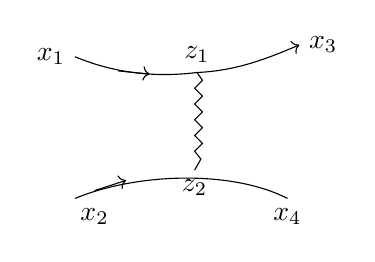
\begin{tikzpicture}[x=1cm,y=1cm]
\draw (0,2.3) .. controls (0.6,2.05) and (1.15,2.05) .. (1.55,2.1);
\draw[->] (0.55,2.12) -- (0.95,2.08);
\draw[->] (1.55,2.1) .. controls (2.05,2.12) and (2.45,2.28) .. (2.85,2.45);
\draw (0,0.5) .. controls (0.8,0.83) and (2.0,0.86) .. (2.7,0.5);
\draw[->] (0.25,0.6) -- (0.65,0.73);
\draw (1.55,2.1) -- (1.62,2.0) -- (1.52,1.9) -- (1.62,1.8) -- (1.52,1.7) -- (1.62,1.6) -- (1.52,1.5) -- (1.62,1.4) -- (1.52,1.3) -- (1.62,1.2) -- (1.52,1.1) -- (1.6,1.0) -- (1.52,0.86);
\node[left] at (0,2.3) {$x_1$};\node[right] at (2.85,2.45) {$x_3$};
\node[below] at (0.25,0.5) {$x_2$};\node[below] at (2.7,0.5) {$x_4$};
\node[above] at (1.55,2.1) {$z_1$};\node[below] at (1.52,0.86) {$z_2$};
\end{tikzpicture}
\end{adjustbox}
\end{center}
Излуч. и поглощ. фотона сопров. множителем $e$.
\begin{equation*}
\int K(x_3-z_1)K(z_1-x_1)K(x_4-z_2)K(z_2-x_2)
D(z_2-z_1)\,d^4z_1\,d^4z_2
\end{equation*}
$D$ — фунд. реш. ур-й Максвелла.

Другие картинки:
\SourceFigure{GELFAND-P000608}{graph-series}{Шесть рисунков в один ряд, разделённых пятью плюсами. Слева две раздельные дуги со стрелками; далее две дуги соединены вертикальной волнистой линией; третий имеет пересекающиеся внутренние штрихи; четвёртый имеет небольшой петлеобразный штрих на волнистой связи; пятый — две волнистые связи с небольшими разрывами у концов; шестой — волнистая связь и неровная петля над верхней линией. Детали пересечения, петлевых стрелок и соединений не уточняются.}
[Под четвёртым рисунком:] рожд. пары.

\begin{equation*}
(\gamma_\mu p_\mu-m)K(p)=1
\end{equation*}
\begin{equation*}
K(p)=\frac{\gamma_\mu p_\mu+m}{p^2-m^2}
\end{equation*}
\begin{equation*}
K(x,x')=\int K(p)e^{ip(x-x')}\,d^4p
\end{equation*}
Полюс обх. если взять
$K(p)=\dfrac{\gamma_\mu p_\mu+m}{p^2-m^2+i0}$

\underline{$p^2=E^2-\vec p^{\,2}$}.
\begin{center}
\begin{adjustbox}{max width=\linewidth}
\begin{tikzpicture}[x=1cm,y=1cm]
\draw[->] (-1.1,0) -- (1.2,0);
\draw[->] (0,-0.45) -- (0,1.1);
\node at (-0.85,0.37) {$\ast$};\node at (0.5,-0.32) {$\ast$};
\end{tikzpicture}
\end{adjustbox}
\end{center}
Если уровни с отр. энергией, соотв. распр. назад по времени
(предсказ. сущ. античастиц).

Сущ. единств. выбор обхода, прив. к согласов. теории: —
\Unclear{GELFAND-P000608}{terminal-words}{ни иметь античастиц?}

\SourcePage{GELFAND-P000609}{unlabelled}

\underline{Нормировка заряда.}

$e$ — явл. ли наблюд. зарядом электрона?

\underline{Рассеяние:} электроны обм. фотонами, сила $\sim e^2$
\begin{center}
\begin{adjustbox}{max width=\linewidth}
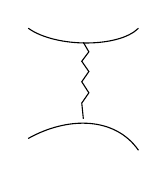
\begin{tikzpicture}[x=1cm,y=1cm]
\draw (-0.7,1.4) .. controls (-0.35,1.15) and (0.45,1.15) .. (0.7,1.4);
\draw (-0.7,0) .. controls (-0.2,0.28) and (0.4,0.28) .. (0.7,-0.15);
\draw (0,1.22) -- (0.07,1.1) -- (-0.02,0.98) -- (0.07,0.85) -- (-0.02,0.72) -- (0.07,0.58) -- (-0.02,0.45) -- (0,0.25);
\end{tikzpicture}
\end{adjustbox}
\end{center}
Поправка:
\SourceFigure{GELFAND-P000609}{correction-loop}{Верхняя и нижняя дуги, между ними почти круговой штрих с двумя стрелкоподобными отметками, короткий вертикальный отрезок сверху и волнистый снизу. У круга слева внизу и под верхним отрезком видны зазоры; соединения через них не додумываются.}
$\sim e^4$.

Наблюд. заряд $e_{\text{физ}}^2<e^2$.

В теор. сильного взаимод. наоборот $g_{\text{физ}}^2>g^2$.

[Разделитель: два горизонтальных штриха с точкой между ними.]

\SourcePage{GELFAND-P000610}{unlabelled}

\underline{\underline{22.9.75.}}\qquad\underline{Сем. Гельфанда.}

[В правом верхнем поле жёлтый значок:]
\begin{adjustbox}{max width=\linewidth}

\begin{tikzpicture}[x=1cm,y=1cm]
\draw[fill=yellow,rounded corners=2pt] (0,0.2) rectangle (0.8,0.75);
\draw[fill=yellow] (0.2,0.2) -- (0.18,0.02) -- (0.4,0.2);
\draw (0.14,0.6) -- (0.66,0.6);\draw (0.14,0.46) -- (0.66,0.46);\draw (0.14,0.32) -- (0.52,0.32);
\end{tikzpicture}
\end{adjustbox}

\underline{Гельфанд о рез. Атьи.}

$\mathcal A$ — все опер. в гильб. пр-ве, $\mathcal K$ — комп. опер.
\begin{equation*}
\mathcal A/\mathcal K=\mathcal B.
\end{equation*}
Когда $B_1,B_2\in\mathcal B$ унитарно эквивалентны?

Это [зачёркнуто: \Unclear{GELFAND-P000610}{cancel-before-brown}{Все?}]
\underline{Браун, Дуглас, Филлмор} (Lect. Notes, N=\ldots)

а) спектры совп. (сущ.)

б) индексы совп. в
\Incomplete{GELFAND-P000610}{cancel-indices}{Зачёркнутая надпись в условии об индексах не восстановлена}
$\forall$ связн. комп. дополнения

\underline{Теор. 2.}
\Incomplete{GELFAND-P000610}{cancel-theorem}{Зачёркнутая надпись перед «Пусть» не восстановлена}
Пусть $X$ — компакт, $\operatorname{Ext}(X)\cong K_1(X)$
[Стрелка к Ext:] мн-во вложений $C(X)$ в $\mathcal B$.

[Разделитель: два горизонтальных штриха с точкой между ними.]
\underline{Мозер} — \underline{Кортевег-де-Фриз}

[Разделитель: два горизонтальных штриха с точкой между ними.]
\underline{Костант}
\begin{equation*}
\psi(x)=\prod_{n=1}^{\infty}(1-x^n);\qquad
\psi(x)^{-1}=\sum_{n=0}^{\infty}p(n)x^n
\end{equation*}
($p(n)$ — число разб. числа $n$).

Это
\begin{equation*}
\psi(x)=\sum(-1)^n x^{\frac{n^2-3n}{2}}
\end{equation*}
\Unclear{GELFAND-P000610}{euler-exponent}{Показатель (n²−3n)/2 сохранён как написано}

[В левом поле крупная чёрная точка.]
«Наиболее замечат. \Unclear{GELFAND-P000610}{function-abbreviation}{ф-ция?}
во всей математике» (Якоби).
\begin{equation*}
(\psi(x))^3=\sum_{n=0}^{\infty}(-1)^n(2n+1)x^{\frac{n(n+1)}2}
\end{equation*}
\begin{equation*}
\eta(x)=x^{1/24}\cdot\psi(x).
\end{equation*}
\begin{equation*}
\eta^{24}(x)=\sum\tau(n)x^n,\qquad
\tau(n)\text{ — ф-я Рамануджана}
\end{equation*}
$\psi^{10}(x)$ тоже есть

Манин: если 6 разных ф-й, получ. из разных соображений

\begin{equation*}
\eta(x)^{\square}=\sum\ldots
\end{equation*}
Макдональд нашёл показ. степени, при к-рых есть смысл:
Это $\dim$ компактных групп Ли.
\begin{equation*}
\psi(x)^{\dim K}=\sum_\lambda
\Incomplete{GELFAND-P000610}{cancel-character}{Зачёркнутый фрагмент слагаемого не восстановлен}
\chi_\lambda(a)\,\dim V_\lambda\cdot x^{\text{(зав. от }\lambda\text{)}}
\end{equation*}
$a\in K$, $\chi_\lambda(a)=\pm1$ или $0$

Костант: $\operatorname{Sp}(-\Delta+a)^{-s}$ и т.д.

\underline{Внутр. \Unclear{GELFAND-P000610}{inner-abbreviation}{ч-ие / ч-во} Г.:}
$\psi(x)^z$ — ?\qquad $(z\in\mathbb C)$

[Разделитель: два горизонтальных штриха с точкой между ними.]
\underline{\underline{Поляков.}} (продолжение).

\underline{Литература:}

[Слева фигурная скобка с подписью \underline{кв. мех.} объединяет пункты 1–4.]

1) \underline{Ландау и Лифшиц} (квант. механика). ($\approx5$–$7$ томов)

2) \underline{Дирак}

3) \underline{Фейнман} (для школьников)

4) \underline{Фейнман}. Интегралы по траекториям

\underline{Кв. теор. поля:} 1-я часть т. \underline{IV}
\underline{Берестецкий, Лифшиц, Питаевский}

\SourcePage{GELFAND-P000611}{unlabelled}

$e(x)$ — поле (биспиноры)
\begin{equation*}
\mathcal L_{\mathrm{free}}=\bar e\,i\gamma_\mu\partial_\mu e
-m\bar e e+\frac1{4e^2}F_{\mu\nu}^2
\end{equation*}
\begin{equation*}
\mathcal L_{\mathrm{int}}=\bar e\gamma_\mu e A_\mu\ldots
\qquad\text{сод. 3-мя. член.}
\end{equation*}

[Разделитель: два горизонтальных штриха с точкой между ними.]
\underline{Локализация
\Unclear{GELFAND-P000611}{heading-abbreviations}{б-их вн.}
симметрий — слабое взаимод.}
\begin{equation*}
\begin{aligned}
\mathcal L={}&\bar e_L i\gamma_\mu\partial_\mu e_L
+\bar e_R i\gamma_\mu\partial_\mu e_R
+\bar\nu_L i\gamma_\mu\partial_\mu\nu_L+\\
&+\begin{pmatrix}e\to\mu\\ \nu_L\to\nu'_L\end{pmatrix}
+m(\bar e_L e_R+\bar e_R e_L).
\end{aligned}
\end{equation*}
(все лептоны)
[От «лептоны» — короткая стрелка к следующей строке.]

$\nu'_L$ — $\mu$-мезонное нейтрино
\begin{equation*}
\mathcal L=\bar e_L i\gamma_\mu\partial_\mu e_L
+\bar\nu_L i\gamma_\mu\partial_\mu\nu_L
+\bar e_R i\gamma_\mu\partial_\mu e_R
\end{equation*}
\begin{equation*}
\left\{
\begin{aligned}
\begin{pmatrix}e'_L\\\nu'_L\end{pmatrix}
&=U\begin{pmatrix}e_L\\\nu_L\end{pmatrix}
\qquad SU_L(2)\\
e'_R&=e_R
\end{aligned}
\right.
\end{equation*}
[В правом поле крупная чёрная точка.]
Возн. новая гр. симметрии $SU(2)$ и ещё $U(1)$
\begin{equation*}
F=SU_L(2)\times U_R(1)\times U_L(1)
\quad\text{— общая лептонная группа.}
\end{equation*}
\begin{equation*}
\begin{pmatrix}e_L\\\nu_L\end{pmatrix}
\overset{U_L(1)}{\longrightarrow}
e^{i\gamma}\begin{pmatrix}e_L\\\nu_L\end{pmatrix}
\end{equation*}
\Unclear{GELFAND-P000611}{phase-letter}{В фазе γ / δ}

\underline{Локализация}

[В левом поле зачёркнуто:]
\Incomplete{GELFAND-P000611}{cancel-left}{Зачёркнутая многобуквенная надпись в рамке не восстановлена}

[Зачёркнуто: $A_\mu$ —
\Incomplete{GELFAND-P000611}{cancel-a}{Средняя часть зачёркнутого определения не восстановлена}
поле.]

Ковар. произв. для $SU(2)$.
\qquad $\vec\tau$ — матр. Паули (3 шт.)
\begin{equation*}
\begin{pmatrix}e'_L\\\nu'_L\end{pmatrix}
=e^{i\frac{\vec\tau\vec\alpha(x)}2}
\begin{pmatrix}e_L\\\nu_L\end{pmatrix},
\qquad E'=e^{i\frac{\vec\tau\vec\alpha(x)}2}E
\end{equation*}
Инфинитезим.:
\begin{equation*}
E'=\left(1-\frac i2(\vec\tau\vec\alpha)\right)E
\end{equation*}
\Unclear{GELFAND-P000611}{finite-infinitesimal-sign}{Знак − в инфинитезимальной записи сохранён}
\begin{equation*}
\partial_\mu E'=
\left(1-\frac i2(\vec\tau\vec\alpha)\right)\partial_\mu E
-\frac i2(\vec\tau\partial_\mu\vec\alpha)E
\end{equation*}
\begin{equation*}
\fbox{$\displaystyle\nabla_\mu E
=\partial_\mu E+\frac i2(\vec\tau\vec A_\mu)E$}
\end{equation*}
\begin{equation*}
E'=e^{i\frac{\vec\tau\vec\alpha(x)}2}E
\end{equation*}
\begin{equation*}
\nabla_\mu E'=e^{i\frac{\vec\tau\vec\alpha}2}\nabla_\mu E
\end{equation*}
Здесь возник. 3 безмасс. частицы

\SourcePage{GELFAND-P000612}{unlabelled}

можно сразу писать
\begin{equation*}
\nabla_\mu E^\delta=\partial_\mu E^\delta+A_\mu^{\delta\beta}E^\beta
\end{equation*}
\Unclear{GELFAND-P000612}{upper-component-index}{Верхний индекс δ / γ}
и смотрим, как преобр. $A$, чтобы $\nabla_\mu E^\delta$ преобр. как $E^\delta$.

\begin{equation*}
\begin{aligned}
\mathcal L_{\mathrm{вз}}={}&(\bar e_i\gamma_\mu\nu_e)A_\mu^{(-)}
+(\bar\nu_e\gamma_\mu e_i)A_\mu^{(+)}\\
&+(\bar e_L\gamma_\mu e_L-\bar\nu_L\gamma_\mu\nu_L)A_\mu^3
\end{aligned}
\end{equation*}
\Unclear{GELFAND-P000612}{weak-electron-index}{Индексы $i$ у электронов сохранены; возможен $L$}
где
\begin{equation*}
A_\mu^\pm=A_\mu^1\pm iA_\mu^2
\end{equation*}
Пример слабого взаимод.: $\mu^-\to e^-,\bar\nu_e,\nu_\mu$.
\begin{equation*}
\mathcal L'=\bar E\left(i\gamma_\mu\frac{\partial E}{\partial x_\mu}\right)
+\bar E\gamma_\mu\vec\tau E\vec A_\mu
+\bar e_R i\gamma_\mu\partial_\mu e_R
\end{equation*}
[Под средним слагаемым — прямая скобка с поднятыми концами.
Под скобкой зачёркнуто прежнее обозначение:]
\Incomplete{GELFAND-P000612}{cancel-underbrace}{Зачёркнутое прежнее обозначение с нижними штрихами не восстановлено}
$\mathcal L_{\mathrm{вз}}$

[В правом поле зачёркнуто:]
\Incomplete{GELFAND-P000612}{cancel-right}{Отдельный зачёркнутый написанный фрагмент не восстановлен}

[Разделитель: два горизонтальных штриха с точкой между ними.]

Ещё локализуем пр. поле
\begin{equation*}
\bar E\left(i\gamma_\mu\frac{\partial E}{\partial x_\mu}\right)
+\bar E\gamma_\mu\vec\tau E\vec A_\mu
+\bar e_R i\gamma_\mu\partial_\mu e_R
+\bar e_R\gamma_\mu e_R B_\mu
\end{equation*}
\begin{equation*}
A_\mu=A_\mu^3\cos\theta+B_\mu\sin\theta
\end{equation*}
[Разделитель: ряд точек и коротких штрихов.]

След. раз — $\approx$ \underline{через 3 недели.}

\textbf{12 кварков:} \underline{4 сорта и 3 цвета.}

[Справа — жёлтая метка в форме пузыря с тремя горизонтальными чёрными полосами.]
\begin{adjustbox}{max width=\linewidth}

\begin{tikzpicture}[scale=.6,line width=.5pt]
\filldraw[fill=yellow,draw=black,rounded corners=3pt]
(0,0)--(0,1)--(1.3,1)--(1.3,0)--(.58,0)--(.3,-.35)--(.36,0)--cycle;
\draw (.22,.75)--(1.07,.75);
\draw (.22,.52)--(1.07,.52);
\draw (.22,.29)--(.83,.29);
\end{tikzpicture}
\end{adjustbox}

[Разделитель: два горизонтальных штриха с точкой между ними.]


\SourcePage{GELFAND-P000613}{unlabelled}
\underline{\underline{29.9.75.}}\qquad\underline{\underline{Сем. Гельфанда.}}

\underline{\underline{Ю.И. Манин.}}
\begin{equation*}
x\prod_{n=1}^{\infty}(1-x^n)^{24}=\sum_{n=1}^{\infty}\tau(n)x^n;
\end{equation*}
$\tau$ — ф-я Рамануджана.

\underline{И.М. Гельфанд}\quad (и Дикий)

$\infty$-мерная алгебра Ли, более замеч., чем все картановские.

[Под всей строкой волнистое подчёркивание.]

Элементы — полиномы $P(u,u',\ldots,u^{(n)})$ от любого числа переменных.

\Unclear{GELFAND-P000613}{formal-variable-mark}{$P[\overset{''}{u}]$}, где $u=\{u,u',\ldots,u^{(n)},\ \}$.

Есть понятие
\begin{equation*}
\frac{d}{dx}P(u,u',\ldots,u^{(n)})
=\sum_{i=0}^{\infty}\frac{\partial P}{\partial u^{(i)}}\cdot u^{(i+1)}
\end{equation*}
Есть умножение (алгеб.)

Неожиданно: есть понятие \underline{коммутатора}:

\Unclear{GELFAND-P000613}{commutator-separator}{$[P,Q]=\displaystyle\sum_{k=0}^{\infty}\left[\left(\frac{d}{dx}\right)^kP\cdot\frac{\partial Q}{\partial u^{(k)}}-\left(\frac{d}{dx}\right)^kQ,\frac{dP}{du^{(k)}}\right]$}

[Зачёркнута короткая запись: \Unclear{GELFAND-P000613}{cancelled-speaker}{неразборчиво}.]
\Incomplete{GELFAND-P000613}{cancelled-speaker-loss}{Короткая зачёркнутая запись перед фамилией Повзнер не восстановлена дословно; сохранившиеся штрихи не дают уверенного слова.}

\underline{\underline{Повзнер.}} Эта ал. связ. с ур-ем $\dfrac{\partial u}{\partial t}=\dfrac{\partial u}{\partial x}$.

Можно связ. с $\forall$ ур-ем
\begin{equation*}
\frac{\partial u}{\partial t}=a(u,u_x,\ldots).
\end{equation*}
Рассм. ф-и $F(u,u_x,\ldots)$ и оператор
\begin{equation*}
a[F(u,u_x,\ldots)]=aF_u+\left(\frac{d}{dx}a\right)F_{u_x}
+\frac{d^2a}{dx^2}F_{u_{xx}}+\ldots
\end{equation*}
Оператор опр. на ф-и $a$ и стр. алгебра из этих опер.
\begin{equation*}
[a,b]=a[b]-b[a]
\end{equation*}
— та же алгебра.

[Слева маленький зачернённый знак.]
Здесь указано существование предст. этой алгебры.

\underline{Манин.} 6 выражений для ф-и Рамануджана $\tau(n)$
(не получ. конечными алгоритмами).

[Слева от пунктов 1 и 2 — обведённый знак $+$. Перед пунктом 3 — два знака $+$ в одной обводке. Номера 1, 2, 3 обведены.]

1. \underline{Определение} $\Rightarrow$
\begin{equation*}
\tau(n)=\sum(-1)^k
\end{equation*}
\begin{gather*}
n-1=n_1+\ldots+n_k,\qquad n_i\ge1,\\
n_1\le n_2\le\ldots\le n_k,
\end{gather*}
подряд $\le24$ знаков рав-ва.

2. \underline{Макдональд} (Дайсон)
\begin{equation*}
\tau(n)=\frac{1}{1!2!3!4!}\sum\prod_{\text{\Unclear{GELFAND-P000613}{vandermonde-relation}{$i<j$}}}(u_i-u_j)
\end{equation*}
\begin{equation*}
10n=\sum_{i=1}^{5}u_i^2,\qquad \sum u_i=0,\qquad u_i\equiv i\mod5
\end{equation*}

3. \underline{Рамануджан}
\begin{equation*}
\tau(n)=\frac{65}{756}\sigma_{11}(n)+\frac{691}{756}\sigma_5(n)
-\frac{691}{3}\sum_{m=1}^{n-1}\sigma_5(m)\,
\end{equation*}
\Unclear{GELFAND-P000613}{ramanujan-convolution}{$\sigma_5(n-n)$}.

[Последняя цифра первого знаменателя 756 переписана.]

$\sigma_k(n)$ — $\sum$ $k$-х степ. делителей числа $n$.

\underline{Следствие:}\quad $\tau(n)\equiv\sigma_{11}(n)\mod691$
\quad (угадал Рамануджан).
\SourcePage{GELFAND-P000614}{unlabelled}
4. Цел. кв. форм с $\det=1$ от 24 перем. всего 2.
Пусть $Q_{24}$ — одна из них.
\begin{equation*}
\tau(n)=\alpha\left(\sum_{Q_{24}=n}1\right)-\beta\sigma_{11}(n)
\end{equation*}
($\alpha,\beta$ вычисл. из $n=1$ и $2$).

5. (Манин)
\begin{equation*}
\tau(n)=\sigma_{11}(n)-\sum_{n=\Delta\Delta'+\delta\delta'}
\left[(\Delta^8\delta^2-\Delta^2\delta^8)
+\frac{691}{6}(\Delta^6\delta^4-\Delta^4\delta^6)\right],
\end{equation*}
\begin{equation*}
\Delta>\delta>0,\quad \text{и }[\Delta'>\delta'>0\quad(\text{целые})
\end{equation*}
или $\Delta\mid n,\ \Delta'=\dfrac n\Delta,\ \delta'=0,\ 0<\dfrac\delta\Delta\le\dfrac12]$.

6. $\sum p(n)x^n=\prod_{n=1}^{\infty}(1-x^n)^{-1}$
($p(n)$ — число разбиений $n$ на произв. число слаг.).
\begin{equation*}
\Rightarrow\quad\sum\tau(n)x^n=x\left(\text{\Unclear{GELFAND-P000614}{partition-inner-start}{$\displaystyle\sum_{n=1}^{\infty}p(n)x^n$}}\right)^{-24}
\end{equation*}
Через $p(n)$ рекурр. нах. $\tau(n)$.

Ф-ла Харди--Рамануджана--Радемахера
\begin{equation*}
p(n)=\frac1{\sqrt3}\sum_{k=1}^{\infty}\frac1{\sqrt k}
\sum_{\substack{h\bmod k\\(h,k)=1}}
\text{\Unclear{GELFAND-P000614}{hrr-omega-exponential}{$\omega_{h,k}e^{-2\pi i n\frac1k}$}}
\frac d{dn}\frac{\operatorname{sh}\frac\pi{6k}\sqrt{24n-1}}{\frac\pi{6k}\sqrt{24n-1}}.
\end{equation*}
$\omega_{h,k}^{24}=1$ тоже есть для $\omega_{h,k}$ явные ф-лы.

Харди--Раманудж. написали [зачёркнуты перекрытые короткие штрихи]
\Incomplete{GELFAND-P000614}{hrr-cancelled-prefix}{Короткая зачёркнутая запись перед sh закрыта штрихами; точные буквы не восстановлены.}
$\operatorname{sh}\to e^{\ldots}$: но если оборвать на члене $\sqrt n$, то приближает хорошо.
[Над строкой вставлено: расходится.]
На $\sqrt n$ членов надо остановиться.
Каждая из этих ф-л — часть беск. серии формул.

7. \underline{\underline{$\tau(mn)=\tau(m)\tau(n)$}}, $(m,n)=1$.
(не видно из ф-л).
\begin{equation*}
\tau(p)=\theta_p+\bar\theta_p,\qquad\theta_p\bar\theta_p=p^{11}
\quad\Rightarrow\quad
\text{\Unclear{GELFAND-P000614}{theta-power}{$\tau(p^a)=\theta_p^a+\bar\theta_p^a$}}.
\end{equation*}
[Правая формула дважды подчёркнута.]
В каждую из ф-л можно подст. и получ. новые тожд.

8. Отсюда $\tau$ — след представления (намного труднее) — Серр, Делинь.
[Над $\tau$ вставлено обведённое: подробнее, что.]
Гротендик, Вейль, Куга, Сато, [зачёркнута короткая запись с петлёй и нижним выносом]
\Incomplete{GELFAND-P000614}{cancelled-author}{Точный текст зачёркнутого фрагмента перед Ранкин не восстановлен; видны петля слева, две горизонтали и нижний выносной штрих.}
Ранкин.
Предст. $\ell$-адическое
\begin{equation*}
\operatorname{Gal}_{\{\ell\}}(\bar Q/Q)\longrightarrow Q_\ell^2
\end{equation*}
(разветвл. только в $\ell$).
След бер. от авт. Фробениуса, порожд. $p$.
Отсюда удалось док., что \underline{\underline{$\theta_p$ чисто мнимые}} (невеществ.)
$\longrightarrow$ Самая длинная теор. в соврем. математике (Оценка Делиня: 2000 страниц).

[На левом поле: у 4 и 5 — по два $+$ в обводке; у 6 — три $+$; у 7 — два $+$; у 8 — четыре $+$ в вертикальной обводке. Номера 4–8 обведены.]
\SourcePage{GELFAND-P000615}{unlabelled}
\underline{Уровни трудности.}
\begin{equation*}
\begin{array}{cl}
+&\text{комбинаторика}\\
++&\text{модулярные формы}\\
+++&\text{комплексный анализ}\\
++++&\text{алг. геом. и т.п., этальные когом. и пр.}
\end{array}
\end{equation*}
[Под последней строкой черта; ниже два коротких штриха.]

\underline{Как получается.}
\begin{equation*}
\text{\Unclear{GELFAND-P000615}{eta-prefactor}{$\eta(z)=e^{\frac{2\pi inz}{24}}\prod(1-e^{2\pi inz})$}}
\end{equation*}
Положим \Unclear{GELFAND-P000615}{x-definition}{$x=e^{\frac{2\pi inz}{24}}$}.
Ф-я хорошо ведёт себя при подст. $z\to\dfrac{az+b}{cz+d}$,
$\left|\begin{matrix}a&b\\c&d\end{matrix}\right|=1$.
\begin{equation*}
\eta(z+1)=e^{\pi i/12}\eta(z),\qquad
\eta(-1/z)=\sqrt{z/i}\,\eta(z).
\end{equation*}
или $\eta^{24}(\tau)(d\tau)^6$ — инв-на отн. др-линейн. подст.
Потеря инф. — $\sqrt[24]{\ldots}=\omega_{c,d}$ — те же.
[Под «Потеря инф.» матрица $\left(\begin{smallmatrix}a&b\\c&d\end{smallmatrix}\right)$.]

Ф-и так. вида (модулярные) — кольцо с 2-мя образ., и надо запис. через образующие,
[над строкой зачёркнуто: или] Тожд. в кольце $\Rightarrow$ рав. в коэфф. Фурье ($\Rightarrow$ 3, 4).
[3 и 4 обведены.]

\underline{\underline{Чистая алгебра:}}
\begin{equation*}
\left\{\varphi(z)\mid\sum_{n=0}^{\infty}a_ne^{2\pi inz}\right\},
\qquad\exists k:\quad
\varphi(z)dz^k\left|\begin{matrix}a&b\\c&d\end{matrix}\right.
=\varphi(z)dz^k.
\end{equation*}
[От множества стрелка к: сх-ся ряд при $\operatorname{Im}z>0$.]
\underline{Т-ма:} кольцо $\Phi=C[E_4,E_6]$.
\begin{equation*}
a_n\big|_{E_4}=\sigma_3(n),\qquad a_n\big|_{E_6}=\sigma_5(n).
\end{equation*}
$\sigma_3$ — суммы кубов делит.

\underline{Х.Р.Р.} (ф-ла 6).
\begin{equation*}
\sum p(n)e^{2\pi inz}=\frac1{\prod(1-e^{2\pi izn})}.
\end{equation*}
Особ. точки на гр. сходимости (полюсы $\infty$ пор. в рац. точках).
Контур интегр. Радемахера: у $\forall$ рац. точки круги опр. радиуса.
\SourceFigure{GELFAND-P000615}{circle-contour}{Над горизонтальной чертой два больших округлых контура, слева и справа; между ними у черты малый округлый контур и короткие дуги. Под чертой метки 0, 1/2, 1. Точная геометрия малых дуг не установлена.}
\begin{center}
\begin{adjustbox}{max width=\linewidth}
\begin{tikzpicture}[x=1cm,y=1cm]
\draw (0,1) .. controls (.45,1.1) and (.7,.75) .. (1,0) .. controls (1.2,.7) and (1.65,1.1) .. (2,1);
\node[right] at (3,.5) {— 1-е прибл.};
\end{tikzpicture}
\end{adjustbox}
\end{center}
\begin{center}
\begin{adjustbox}{max width=\linewidth}
\begin{tikzpicture}[x=1cm,y=1cm]
\draw (0,1) .. controls (.7,.6) and (.9,.25) .. (1.25,-.25) -- (.75,-.25) .. controls (.9,.4) and (1.35,.8) .. (2,1);
\node[right] at (3,.5) {— 2-е прибл.};
\end{tikzpicture}
\end{adjustbox}
\end{center}
и т. д.
[Ниже горизонтальная черта.]

Частн. случай ф-л Макдональда в преобр. Костантом виде:
\begin{equation*}
\varphi(x)=\prod_{n=1}^{\infty}(1-x^n),\qquad
\varphi(x)=\sum_{\lambda\in D}\chi_\lambda(a)\dim V_\lambda\,x^{c(\lambda)}.
\end{equation*}
[Под первой формулой зачёркнута короткая запись.]
\Incomplete{GELFAND-P000615}{kostant-cancelled}{Короткое зачёркнутое слово под произведением закрыто плотными горизонтальными штрихами; видны начальная дуга и нижние штрихи.}
[$D$: старш. веса непр. предст.; под $\chi_\lambda(a)$ написано $0,\pm1$.]
\begin{equation*}
c(\lambda)=(\lambda+\rho,\lambda+\rho)-(\rho,\rho).
\end{equation*}
\SourcePage{GELFAND-P000616}{unlabelled}
\underline{$6/\bar X-75$}\qquad\underline{Сем. Гельфанда.}
[У верхнего правого края на уровне даты видны обрезанные нижние части письменной строки: p-подобный начальный фрагмент и ряд коротких штрихов.]
\Incomplete{GELFAND-P000616}{top-right-trace}{Строка у верхнего правого края обрезана; полные буквы и слова недоступны.}

Лерэ.
[Под именем зачёркнутая запись с петлями и горизонтальной штриховкой.]
\Incomplete{GELFAND-P000616}{leray-cancelled}{Точные буквы зачёркнутой записи под Лерэ не восстановлены.}
«5 лет назад Арнольд предложил мне почесть одну книгу Маслова».
«Теперь я начинаю понимать, к чему ведёт эта книга».
\underline{Алгебрич. предпосылки к раб. Маслова,}
в част. Метаплектич. группа Буслаева.
Маслов: $X=R^\ell$, Буслаев $X$ — любое мн-зие.
\begin{equation*}
X=R^\ell:\quad S(X),\ S'(X),\ H(X)\text{ — промежут. гильб. пр-во.}
\end{equation*}
\begin{equation*}
a\left(x,\frac1\nu\frac\partial{\partial x}\right),\qquad\frac\nu i\in R_+.
\end{equation*}
Пусть вначале $a$ — лин. [зачёркнута короткая запись с петлёй и нижним выносом]
\Incomplete{GELFAND-P000616}{linear-cancelled}{Зачёркнутое слово после лин. закрыто густыми штрихами; точные буквы не установлены.}
по обоим аргументам.
Ищем гр. автоморф. $S'(X)$.
\begin{equation*}
S:f'\longrightarrow Sf',\qquad SaS^{-1}\in A.
\end{equation*}
($A$ — [зачёркнуто слово с рядом низких дуг]
\Incomplete{GELFAND-P000616}{operator-class-cancelled}{Зачёркнутое слово между A — и класс опер. не восстановлено.}
класс опер., линейных по $x$ и $\partial/\partial x$.)
\underline{Пример:} $\widehat F$, $\widehat F^{-1}$ и $\widehat F$ по неск. коорд.
лин. замена перем. в $X$-пр-ве.
$S$ — сохр. автом. $A$ (внутр.).
\begin{equation*}
a:X\oplus X^*\longrightarrow C
\end{equation*}
[$a(x,p)$ написано ниже.]
гр. автом. — симпл. группа
\begin{equation*}
\langle p',x\rangle-\langle p,x'\rangle.
\end{equation*}
\begin{equation*}
X\oplus X^*=Z(\ell).
\end{equation*}
$G(\ell)$ — гр. автом. в пр-ве распр. $\Rightarrow$ получ. её предст.
\begin{equation*}
G(\ell)\longrightarrow\operatorname{Sp}(\ell),\qquad
\text{ядро: }\dot C,\qquad G(\ell)/\dot C=\operatorname{Sp}(\ell).
\end{equation*}
$c\in\dot C=C\setminus0$.
В частности, $G(\ell)$ — гр. Ли.
\SourcePage{GELFAND-P000617}{unlabelled}
Изв. много элем. — полн. и частич. пр. Фурье.
\begin{equation*}
A:X\oplus X\longrightarrow R\quad\text{квадр. вещ.},\qquad
\Delta(A)=\sqrt{\det A(x,x')}\ne0.
\end{equation*}
\begin{equation*}
(S_Af')(x)=c\left(\frac{|\nu|}{2\pi i}\right)^{\ell/2}\Delta(A)
\int_Xe^{\nu A(x,x')}f'(x')\,d^\ell x'.
\end{equation*}
\begin{equation*}
(x,p)=s_A(x',p')\quad\Leftrightarrow\quad p=A_x,\ p'=-A_{x'}
\end{equation*}
— соотв. симпл. преобразование.
$S$ — унит. оператор.
Унитарность $\Rightarrow$ метапл. группа $M_p(\ell)$.

I. Segal; A. Weil; K. Siegel.
Мат. физ. произв. норм $\longrightarrow$ для полн. раб. Зигеля.
\begin{equation*}
M_p(\ell)\ni
\end{equation*}
\Incomplete{GELFAND-P000617}{mp-cancelled}{Между знаком принадлежности и S с индексом A зачёркнута письменная запись; видны начальный вынос и тёмные горизонтали, точные буквы не восстановлены.}
\begin{equation*}
S_A\longmapsto s_A.
\end{equation*}
это ф-ла с $|c|=1$.
Возьмём $c=\pm1$.
\begin{equation*}
S_A\cdot S_{A'}=S_{A''}
\end{equation*}
[Перед следующей формулой зачёркнута короткая запись.]
\Incomplete{GELFAND-P000617}{sign-cancelled}{Короткое зачёркнутое слово перед S с индексом A закрыто горизонтальными штрихами; точные буквы не отделены.}
\begin{equation*}
\underline{S_AS_{A'}S_{A''}=\pm E}
\end{equation*}
[Ниже $s_As_{A'}s_{A''}=e$, стрелка вверх к подчёркнутой формуле.]
знак $\sim$ инд. Маслова.
Разложим:
\begin{equation*}
A(x,x')=\langle Px,x\rangle-\langle Lx,x'\rangle+\langle Qx',x'\rangle,
\qquad P,Q,L:X\longrightarrow X'.
\end{equation*}
[Под формулой ряд точек и короткий перечёркнутый штрих слева.]
\SourcePage{GELFAND-P000618}{unlabelled}
\underline{13.10.75. Сем. Гельфанда.}

\underline{Фрадкин.} (Ефим \Incomplete{GELFAND-P000618}{patronymic-cancelled}{Зачёркнутое слово перед «Самойлович».} Самойлович).

Что надо знать?
\begin{enumerate}
\item \underline{Квант. механика}: Ландау.
\item \underline{Теория поля}: Боголюбов, Ширков; Ахиезер и Берестецкий;
Паули — старые. Фрадкин, Труды ФИАН, т.29 (стар.)
(теор. поля и стат. из функц. подхода), $S$-матр и т.д.
[От «т.29 (стар.)» стрелка вниз к «коротка.»]
\item \underline{Теория предст. групп}: Гельфанд, Минас, Шапиро.
\item \underline{Антикоммут. пер.} (Ферми-пер.): Березин; метод втор. квантов.
\item Абрикосов, Г\Incomplete{GELFAND-P000618}{covered-name}{Часть фамилии закрыта жёлтым значком; видимы начало и «орьков».}орьков,
Дзялошинский, «Методы теории поля в стат. физике» (книга).
\item «Калибровочные поля» \Unclear{GELFAND-P000618}{bib6-authors}{Коноплёв} и Пенков.
\item Обзоры Вайнберга, Ли и др. в
\end{enumerate}

\underline{Переломов. О вполне инт. гам. системах.}
($\exists n$ первых инт. в инволюции)
\begin{equation*}
H=\frac12\sum_{k=1}^{n}p_k^2+U(q_1,\ldots,q_n).
\end{equation*}
Г. Теор. Лиувилля: сист. тогда реш. в квадратурах.
$H=\frac12p^2+\sin q$; 2-й инт. — эллипт. ф-я.

\underline{0-й пример} — \Incomplete{GELFAND-P000618}{toda-first-cancelled}{Зачёркнутые слова перед «цепочка».}
\underline{цепочка} \Incomplete{GELFAND-P000618}{toda-second-cancelled}{Зачёркнутое слово перед «Тода».} Тода.
\begin{equation*}
\text{\Unclear{GELFAND-P000618}{toda-potential}{$U=g^2\sum_{k=1}^{n}\bigl(e^{-(q_{n+1}-q_n)}-e^{-(q_n-q_{n-1})}\bigr)$}},
\qquad q_{k+n}=q_k.
\end{equation*}
\Incomplete{GELFAND-P000618}{manakov-date-cancelled}{Зачёркнутая запись перед «С. Манаков».}
С. Манаков $\xi$ 1974; Toda 1970 (Prog. Th. Ph.);
1973 Hénon, Flaschka \Incomplete{GELFAND-P000618}{flaschka-date-cancelled}{Зачёркнутая дата.} 1974
$\longrightarrow$ были инт., но не яс., что в инвол.
М. Кас, van Moerbeke 1975.
[Справа зачёркнуто: «1975 Мозер J. Moser (препр.)».]

А:
\begin{equation*}
U=g^2\sum_{k<\ell}V(q_k-q_\ell).
\end{equation*}
Г. \underline{Задачи}: а) найти инт. б) док., что в инвол.
в) реш. обр. задачу г) выпис. инт. в квадратурах.

Б:
\begin{equation*}
U=g^2\sum_{k<\ell}[V(q_k-q_\ell)+\varepsilon V(q_k+q_\ell)]
+g_1^2\sum V(q_k)+g_2^2\sum V(2q_k).
\end{equation*}
[Правая часть последней скобки у края кадра.]
\begin{equation*}
\begin{array}{c|l|l|l|c|l}
 &V(q)&I_k&\{I_k,I_\ell\}=0&I.P.\ (\text{обр. задача})&x(q)\\
1&q^{-2}&M,OP&M,OP&?&q^{-1}\\
2&a^2\operatorname{sh}^{-2}aq&CMR,OP&CMR,OP&?&a\operatorname{cth}aq\\
3&a^2\sin^{-2}aq&M,OP&CMR,OP&?&a\operatorname{ctg}aq\\
4&a^2\wp(aq\mid\omega_1,\omega_2)&C,OP&\text{\Unclear{GELFAND-P000618}{table-cancelled}{$?\ ?$}}&?&a\frac{\operatorname{cn}aq}{\operatorname{sn}aq}\\
5&q^{-2}+a^2q^2&P,P&P,P&?&
\end{array}
\end{equation*}
\Incomplete{GELFAND-P000618}{table-cancelled}{Перед вопросительными знаками в четвёртой строке зачёркнута короткая запись.}
$\wp$ — ф-я Вейерштрасса. 2,3 — пред. случаи 4.
1 столбец — А; 2 — Б.
[Таблица разделена вертикальными чертами; под заголовком горизонтальная черта.]
[Между таблицей и последней записью зачёркнуты короткие штрихи, похожие на $\ell\sum$.]
\SourcePage{GELFAND-P000619}{unlabelled}
1975 J. Moser препр.
F. Calogero, M., R., (3 авт.) Lett. Notes.
\begin{equation*}
\left.\begin{array}{ll}
&\text{Calogero}\\
OP&\text{Ольшанецкий, Переломов}\\
P&\text{Переломов}
\end{array}\right\}\ \text{по иниц.}
\end{equation*}
Коулмен, Шроер — связь с \Incomplete{GELFAND-P000619}{coleman-cancelled}{Зачёркнутая запись перед «мод. Тирринга».}
мод. Тирринга с sin-Гордон.
0 — обр. зад. — Склянин.
\begin{equation*}
0\qquad g^2\sum_{k=1}^{n}e^{-(q_{k+1}-q_k)}.
\end{equation*}
Обратная задача нигде не решена (кроме случ.0).
\underline{Инт. имеют вид всегда} $I_k=\operatorname{Sp}(L^k)$,
где явный вид $L$ выписывается ($L$-матрица).
[Слева двойная черта и вертикально: «типы 1–4».]
\begin{equation*}
L=P+iX;\quad P_{k\ell}=p_k\delta_{k\ell},\quad
X_{k\ell}=(1-\delta_{k\ell})x(q_k-q_\ell),
\end{equation*}
$P$ — диаг. матр.; где $x(q)$ выпис. в таблице.
Обр. зад. здесь: по следам степеней найти элем. матрицы.
Идея: от Лакса в КдФ.
\begin{equation*}
N=5\quad I_k=\operatorname{Sp}(N^k),\quad N=L^2+\omega^2Q^2,
\qquad Q_{ij}=q_j\delta_{ij}.
\end{equation*}
Манаков — конечномерн. аналог высш. КдФ, разоб. первые два. (дисс.)
Квант. сист. тоже разоб., тоже предст. интерес.
$p=-i\dfrac{\partial}{\partial q}$.
Тогда $H=$ опер. Лапласа на симм. пр-ве (радиальная часть).
Экв. сист.3 — квантованный.

\underline{Вопр. Гельфанда}: нельзя ли всё свести к групповой интегр., но в более широком пр-ве.
\underline{Связь со сх. Дынкина}: $\{\alpha\}$ — корни, $q_\alpha=(\alpha,q)$.
\begin{equation*}
U=\sum_{\alpha>0}g_\alpha^2V(q_\alpha),\qquad
g_\alpha=g_\beta,\ \text{если длины }\alpha\text{ и }\beta\text{ равны}.
\end{equation*}
$\alpha_{ij}=e_i-e_j$ — получ. сист. Мозера.
А — сист. корней типа $A_n$.
Б — при разн. знач. const $B,C,BC,D$ и т.д.
\Incomplete{GELFAND-P000619}{bottom-cancelled}{Зачёркнутая короткая запись перед «Есть».}
Есть и все особ. группы. Неясно пока, явл. ли сист. особ. групп вполне интегрир.

\underline{Фрадкин. Е.С.} Что нового за последние 20 лет?
1. Рассм. произв. систему. Она зад. лагр. или гамильтонианом $H(p,q)$ (пока классический).
$p,q$ могут быть ферми и бозе (смесь).
[Справа: $p,q$ — либо бозевские, либо грассмановские (ферми),
стрелка вниз к $pq+qp=1$. (см. Березин).]
Есть ещё связи $\varphi_k(p,q)=0$ [последняя буква $q$ написана поверх прежних штрихов].
(отличить между пер. бозе и ферми).
\underline{Пример}: калибров. поля (эл.-динамика $(A_{00})$, Янг-Миллс,
гравит. поле, ур. Эйнштейна), град. инв. ур-й Максвелла.
а свет был в $2^{\text{х}}$ сост., а не $3^{\text{х}}$, лишн. убир. калибр. инв.
[Справа: все поля с высш. спинами.]
\begin{equation*}
\varphi_k=0\quad\text{бозе связи},\qquad
\chi_k=0\quad\text{ферми связи}.
\end{equation*}
\SourcePage{GELFAND-P000620}{unlabelled}
[Сверху слева: \Unclear{GELFAND-P000620}{top-measures}{$\prod(d\varphi,d\pi,d\psi,d\pi^{(\psi)})$}.]
Лагранжиан $L(q,\dot q)$, $p=\dfrac{\partial L}{\partial^r\dot q}$.
\underline{Скобки Пуассона}: ($r$ — учит. правую производную).
\begin{equation*}
\{A,B\}=\frac{\partial A}{\partial^r q}\frac{\partial B}{\partial^\ell p}
-(-1)^{n_A n_B}\frac{\partial B}{\partial^r q}\frac{\partial A}{\partial^\ell p}.
\end{equation*}
$n_A=0$, если число Ферми-пер. чётное (в $A$);
$n_A=1$ — нечётное.
Невырожденность: $\dot q=f(q,p)$ (можно выразить).
Иногда нельзя, когда $\det\dfrac{\partial^2L}{\partial\dot q_i\,\partial\dot q_j}=0$.
Тогда возникают доп. связи.
Можно дальше действ. в том же духе и получить (см. тонкую книгу Дирака)
все связи \Incomplete{GELFAND-P000620}{constraints-cancelled}{Зачёркнутое слово.}
Замыкаем отн. скобки Пуасс. (до алг. Ли).
$\psi_k$ — доп. условия, к-рые так получаются.
\underline{Дирак}: [обведено «важно»] связи 2-го рода, между к-рыми
$\{\varphi_k,\psi_j\}\ne0$ с учётом доп. условий.
Выбрав связи, принадл. центру и т.д.
\underline{Произв. ф-л всех ф-й Грина}.
[Зачёркнута вся строка:
\begin{equation*}
Z=\int d\varphi_j\,d\pi_j^{(\varphi)}\,
\end{equation*}
\Incomplete{GELFAND-P000620}{z-cancelled}{Плотно зачёркнутый множитель меры.}
\begin{equation*}
d\pi_j^{(\psi)}\,\delta(\varphi_k)\delta(\chi_k)\exp.
\end{equation*}
]
\begin{equation*}
\begin{aligned}
Z={}&\frac1C\int\prod_x d\varphi_j(x)\,d\pi_j^{(\varphi)}(x)\,
d\psi_j(x)\,
d\pi_j^{(\psi)}(x)\,\delta(\varphi_k)\delta(\chi_k)\times\\
&\times\exp\left\{\int_{\mathbb R^4}
\pi_j^{(\varphi)}\dot\varphi_j+\pi_j^{(\psi)}\dot\psi_j
-H(\pi^{(\varphi)},\varphi,\psi,\pi^{(\psi)})\right.\\
&\left.\qquad -\pi_j\bar I_j^{(\varphi)}-\varphi_j I_j^{(\varphi)}
-\pi_j^{(\psi)} I_j^{(\psi)}
-\text{\Unclear{GELFAND-P000620}{last-source-term}{$\bar I_i^{(\psi)}\psi_j$}}\right\}d^4x+A.
\end{aligned}
\end{equation*}
\Unclear{GELFAND-P000620}{z-exponent-grouping}{$\exp\{\int\ldots\}d^4x+A$}.
где
\begin{equation*}
\text{\Unclear{GELFAND-P000620}{a-grouping}{$
A=\exp\left(-\frac{\delta(0)}2\right)\operatorname{Tr}
\left\{\ln\{\chi_i,\chi_j\}_+
-\operatorname{Tr}\ln\left[\{\varphi_i,\varphi_j\}_-
-\{\varphi_i,\chi_j\}_-\{\chi_i,\chi_j\}_+^{-1}\{\chi_i,\varphi_j\}_-\right]\right\}$}}.
\end{equation*}
[Второе $\operatorname{Tr}$ вставлено над строкой с V-образным знаком вставки.]
$\varphi$ — бозе-поля; $\psi$ — ферми-поля.
$\operatorname{Tr}$ от матриц.
(Общая ф-ла всех квантовых теорий).
$\varphi,\chi$ — связи (только некоммутирующие).
$I$ — «источник», $\varphi$ и $\psi$ — элем. сопр. пр-ва.
Получ. аналог преобразования Фурье.
$A$ — член, связ. со связями.
$\delta(0)$ потом сократится (в $S$-матрице).
$\{\chi,\chi\}_{\pm}$ — скобки Пуассона (Бозе и Ферми).
[Внизу две горизонтальные черты.]
\SourcePage{GELFAND-P000621}{unlabelled}
\underline{20/X-75. Сем. Гельфанда.}
\underline{И.М. Гельфанд}:
\begin{equation*}
L=-\frac{d^2}{dx^2}+u(x),\qquad A=\frac{d^3}{dx^3}+\ldots,\qquad [L,A]=K(u).
\end{equation*}
$A=L^{3/2}$ с обрез. недифференц. членами.
\underline{1-зонный потенциал}: $K(u)=0$.
Суть (гипотеза): для $u$ операторы $L$ и $A$ коммутируют.
Высшие ур-я: $A=L^{5/2},L^{7/2},\ldots$;
почти коммутир. — ост. опер., умн. на ф-ю.
\Incomplete{GELFAND-P000621}{hypothesis-prefix-cancelled}{Зачёркнутая короткая запись слева перед «Гипотеза».}
Гипотеза: это кусок недоделанной некоммут. теории.
Кричевер: фактич. исходил из этого.
\Incomplete{GELFAND-P000621}{krichever-cancelled}{Зачёркнутая короткая запись слева от имени.}
\underline{Кричевер. Игорь.}
Рассм. операторное ур-е $[L_n,L_m]=0$, где
\begin{equation*}
\begin{aligned}
L_n&=\sum_{i=0}^{n}u_i(x)\frac{d^i}{dx^i},\qquad u_n(x)\equiv c_0,\ u_{n-1}\equiv c_1,\\
L_m&=\sum_{i=0}^{m}v_i(x)\frac{d^i}{dx^i}.
\end{aligned}
\end{equation*}
[Справа зачёркнуто: \Unclear{GELFAND-P000621}{solution-cancelled}{$v_m(x)$}.]
$v_m$ и $v_{m-1}$ тоже const. (всегда рассматриваются такие операторы).
Напишем сист. ур-й:
\begin{equation*}
0=\sum_{k,\ell}u_k C_k^{k+\ell-s}v_\ell^{(k+\ell-s)}
-\sum_{k,\ell}v_k C_k^{\ell+k-s}u_\ell^{(\ell+k-s)},
\qquad 0\le s\le m+n-3.
\end{equation*}
Число ур-й $=$ числу неизвестных.
\begin{equation*}
mu'_{n-2}-nv'_{m-2}=0\quad\Rightarrow\quad
v_{m-2}=\frac mn u_{n-2}+h_2\qquad(h_2=\mathrm{const}).
\end{equation*}
Легко пров., что 1-е [(m−1), над строкой с дугой к «ур-й»] ур-й
(при $n-1\le s\le m+n-3$) позв. выразить все $v_i$ в виде полиномов от $u_i$
(и их производных). Ещё \Incomplete{GELFAND-P000621}{equation-cancelled}{Зачёркнутая короткая запись.}
возникает постоянные интегрирования.
Подставляя их в ур-я $0\le s\le n-2$, мы получим ур-й на \Unclear{GELFAND-P000621}{coefficient-overwrite}{$u_i$} коэфф. $L_n$.
Для $L=-\dfrac{d^2}{dx^2}+u(x)$ получается при $m=2k+1$ набор опер.,
\Incomplete{GELFAND-P000621}{constant-cancelled}{Зачёркнутое слово перед «у к-рых».}
у к-рых коммутатор — умн. на ф-ю. На $u$ остаётся 1 ур-е — высшее ур-е КдФ.
Сем-во с \Incomplete{GELFAND-P000621}{family-cancelled}{Зачёркнутая запись.}
зависит от const интегрирования.
\underline{Теорема (А.Б. Шабат)}. Если
\Incomplete{GELFAND-P000621}{shabat-cancelled}{Зачёркнутая гипотеза перед «для».}
для $L_n$ сущ. опер. $L_m$: $[L_n,L_m]=0$, то $\exists$ полином $P(x,y)$:
\begin{equation*}
P(L_n,L_m)=0.
\end{equation*}
(коммутативный).
\SourcePage{GELFAND-P000622}{unlabelled}
\underline{Док-во}.
[Зачёркнуто: \Unclear{GELFAND-P000622}{top-cancelled}{они простые при $(n,m)=1$}.]
Пусть $y$ — решение ур-я:
\begin{equation*}
L_n y=Ey;\qquad y_j(x,E)\text{ — базис реш. (целые ф-и от }E\text{)}.
\end{equation*}
\begin{equation*}
\text{\Unclear{GELFAND-P000622}{initial-condition}{$y_i^{(j)}(x_0,E)\quad\delta_{ij}$}}.
\end{equation*}
$L_m$ задаёт лин. опер. в пр-ве решений ур-я $L_n y=Ey$ $(\forall E)$.
Хар. полином его:
\begin{equation*}
\text{\Unclear{GELFAND-P000622}{characteristic-degree}{$0=L_m^{n+1}(E)+r_n(E)L_m^n(E)+\ldots+r_0(E)$}}.
\end{equation*}
Коэфф. — целые ф-и от $E$.
Док., что они полиномы по $E$. Это следствие асимптотики $y_i(E)$ по $E$ (при $E\to\infty$).
\begin{equation*}
y_i(x,E)\sim\sum_{j=0}^{n-1}a_{ij}e^{\varepsilon_j kx};
\qquad \varepsilon_j^n=1,\quad k^n=E.
\end{equation*}
Отсюда степень роста $r_j(E)\le$ полин. от $k$ $\Rightarrow$ они сами полиномы.
\begin{equation*}
r_j(E)y=r_j(L_n)y.
\end{equation*}
Отсюда хар. полином $P(L_n,L_m)y=0$.
[Обведено с указателем: «беск. мерное пр-во».]
Но решений дост. много ($E\to\infty$) $\Rightarrow P(L_n,L_m)=0$. $\triangleright$
\underline{И. Бернштейн}: для полиномиальн. коэфф. было в Ф.А. т.1, №4.
[Зачёркнута строка:
\Incomplete{GELFAND-P000622}{baker-cancelled}{Зачёркнутое слово в начале строки.}
\Unclear{GELFAND-P000622}{baker-cancelled-formula}{$\psi_i(0,E)=\delta_i$}.]
Пусть $\psi_i(x,E)$ соб. для пары оп.:
\begin{equation*}
L_n\psi_i(x,E)=E\psi_i(x,E),\qquad
L_m\psi_i(x,E)=E_i\psi_i(x,E).
\end{equation*}
Тогда рассм. пов.
[Слева заштриховано: \Unclear{GELFAND-P000622}{left-cancelled}{$\psi(x,P)$}.]
\begin{equation*}
\underline{P(x,y)=0},\qquad x,y\text{ — соб. знач. }L_n\text{ и }L_m.
\end{equation*}
$\Rightarrow E_i$ алг. ф-и от $E$.
[Справа: $\psi|_{x_0}=1$ (нормир.).]
\underline{$\Psi(x,P)$} — ф-я на этой пов.
\Unclear{GELFAND-P000622}{function-cancelled}{BAKER}
\Incomplete{GELFAND-P000622}{function-cancelled}{Заштрихованное слово после «пов.» не прочитано полностью.}
$P\in X$.
[Под записью две горизонтальные черты.]
Рассм. $\forall$ неособ. алг. кривую $X$ с отм. точкой $P_0\in X$.
\underline{След. св-ва однозн. задают ф-ю $\Psi(x,P)$}, $x\in(a,b)$,
$P\in X$. (Ахиезер).

$1^\circ$. $\psi(x,P)$ мероморфно в
\Unclear{GELFAND-P000622}{first-cancelled}{$x_0$} [зачёркнуто] $X\setminus P_0$,
имеет дивизор полюсов $D$ с $\operatorname{deg}D=g$, причём $D$ неособый и не зависит от $x$.

$2^\circ$.
\begin{equation*}
\psi(x,P)=e^{k(x-x_0)}\left(1+\sum_{i=1}^{\infty}
\frac{\text{\Unclear{GELFAND-P000622}{series-numerator}{$\xi_i(x)$}}}{k^i}\right),
\qquad\frac1k=z\text{ — лок. параметр в окр. }x_0.
\end{equation*}
[Под скобкой: «регулярная ф-я в окр. $P_0$».]


\SourcePage{GELFAND-P000623}{unlabelled}
Введём кольцо $\Lambda(X,P_0)$ ф-й, рац. на кривой $X$ с единств. особ. в т. $P_0$.

\underline{Теорема.} $\forall E\in\Lambda(X,P_0)$, $\exists!$ дифф. опер. $L$, такой что
\begin{equation*}
L\Psi(x,P)=E(P)\Psi(x,P).
\end{equation*}
[Зачёркнута надпись; возможное начало «Д-во».]
\Incomplete{GELFAND-P000623}{crossed-top}{Продолжение зачёркнутой надписи не читается.}
При этом если $E(P)=c_nk^n+c_{n-1}k^{n-1}+\ldots+c_0+\ldots$
($1/k$ — лок. пар. в окр. $P_0$), то
\begin{equation*}
L=c_n\frac{d^n}{dx^n}+c_{n-1}\frac{d^{n-1}}{dx^{n-1}}+
\sum_{i=0}^{n-2}u_i(x)\frac{d^i}{dx^i}.
\end{equation*}
[Нижний предел суммы обведён и исправлен.]
Где $u_i$ — нек-рые ф-и.

\underline{Д-во.}
\begin{equation*}
\Psi(x,P)=e^{k(x-x_0)}\left(1+\sum_{i=1}^{\infty}\frac{\xi_i(x)}{k^i}\right).
\end{equation*}
Дифф. по $x$: полюса те же
(тот же дивизор), а в окр. $P_0$
(применим $L$) получ.
\begin{equation*}
\frac{d}{dx}\Psi(x,P)=k\Psi+e^{k(x-x_0)}
\left(\sum_{i=\Unclear{GELFAND-P000623}{proof-sum}{0}}^{\infty}\frac{\xi'_i(x)}{k^i}\right),
\end{equation*}
т.е. получ. новый полюс в т. $P_0$.
Ищем $L$ из усл. совпад. син. частей $L\Psi$ и $E\Psi$.
Получим:
\begin{equation*}
u_i(x)=Q\left(c_j,\frac{d^{\Unclear{GELFAND-P000623}{coefficient-order}{n}}}{dx^n}\xi_s(x)\right),
\qquad 0\le s\le i-1,\quad 0\le r\le i-s;
\end{equation*}
т.е. $u_i$ явно нах. из асимптотики.
Отобр. $E\longrightarrow\Unclear{GELFAND-P000623}{map-crossed}{L}$
[Буква в конце стрелки переправлена.]
Это кольцевой гомоморфизм
\begin{equation*}
\varphi:\Lambda(X,P_0)\longrightarrow\mathcal L\qquad(\text{дифф. опер.}).
\end{equation*}
Образ — коммут. кольцо.
[Слева вставлено:] Пусть $n$ — наим. возможное,
Пусть $\mu_1,\ldots,\mu_{n-1}$ — такие числа, что $\exists\psi$ с полюсом пор. $s+\mu_sn$.
\begin{equation*}
\mu_1+\ldots+\mu_{n-1}=g.
\end{equation*}
В точке общ. полож. — $g$ алгебраич. независимых коммутир. операторов.

\underline{Опр.} Дифф. оп. $L_n$ наз. алгебр. рода $g$, если он возникает в этой конструкции.

\underline{Теорема.} $L_n$ — алг. рода $\le\Unclear{GELFAND-P000623}{genus-index}{g}$
$\Longleftrightarrow\exists$ операторы $L^{(s)}$, $1\le s\le n-1$, такие что
\begin{equation*}
[L_n,L^{(s)}]=0;\quad [L^{(s)},L^{(1)}]=0,\qquad
\operatorname{ord}L^{(s)}=s+\mu_sn,
\end{equation*}
где $\mu_i$ таковы, что $\mu_1+\ldots+\mu_{n-1}=g$.
\SourcePage{GELFAND-P000624}{unlabelled}
\underline{Замеч.} Если оп. коммут. с парой, то коммут. между собой.
\underline{Д-во:} а) необх. очевидна ($L^{(s)}$ — обр. базисных ф-й) из предыд.
б) достат. — [зачёркнуто; видны фрагменты «кон…»]
\Incomplete{GELFAND-P000624}{crossed-suff}{Зачёркнутые слова перед «строим» не восстановлены.}
строим из соб. знач. ф-и на кривой; дост. для рода $g$. $\square$

\underline{Лиманов:} если 2 опер. с полин. коэфф. коммут. с
$\Unclear{GELFAND-P000624}{lemma-exponent}{z^m}$, то они коммут. между собой
(опер. от 1-го перем.).

\underline{Конструкция $\Psi$:}
\begin{equation*}
\Psi(x,P)=\exp\left\{\int_{P_0}^{P}\omega\right\}
\frac{\Theta\bigl(\overline{\omega_\nu(P)}-e_\nu+U_\nu x\bigr)}
{\Theta\bigl(\omega_\nu(P)-e_\nu\bigr)}.
\end{equation*}
\begin{equation*}
\omega_2=\frac{dz}{z^2}\quad(\text{выбор }k\text{ таков})
\end{equation*}
[Под «выбор $k$» вставлено: «или $z$».]
\begin{equation*}
\omega_\nu(P)=\int_{P_0}^{P}\omega_\nu;
\qquad\omega_\nu\text{ — аб. дифф. на кривой}.
\end{equation*}
\begin{equation*}
\omega_\nu(P)=\int_{P_0}^{P}\omega_\nu,\quad
\int_{a_i}\omega_\nu=\delta_{i\nu},\qquad
B_{\mu\nu}=\int_{b_\mu}\omega'_\nu.
\end{equation*}
\begin{equation*}
\Theta(u_1,\ldots,u_n)=\sum_{m_1,\ldots,m_n}
\exp\left\{2\pi i\,\Unclear{GELFAND-P000624}{theta-crossed}{[зачёркнутый знак]}
\sum_{\mu,\nu}B_{\mu\nu}m_\mu m_\nu+\sum_\nu m_\nu u_\nu\right\}.
\end{equation*}
\SourcePage{GELFAND-P000625}{unlabelled}
\underline{27/X-75.} \underline{Сем. Гельфанда.}

\underline{Дубровин.}

$\forall$ опер. $L$ $\exists$ серия ур-й типа КдФ.
\begin{equation*}
L=\frac{d}{dx}+U(x),\qquad U(x)\text{ — матр. }n\times n.\quad (u_i^j(x))\qquad(1)
\end{equation*}
Ур-е будет
\begin{equation*}
\dot U=K_{\text{\Unclear{GELFAND-P000625}{flow-index}{N / m}}}(U);\qquad m=1,2,\ldots\qquad(2)
\end{equation*}
\textit{[Под $K$:]} нелин. дифф. оп. по $x$.

\underline{$K_m(U)=0$} — вполне инт. гам. сист., к-рая явно решается.
Допуск. коммут. предст. типа Лакса на матрицах $\Lambda'=[\Lambda,Q]$.
(матр. элем. $\text{\Unclear{GELFAND-P000625}{poly-overwritten}{Λ / U, исправлено}}$ — полиномы от $U,U',\ldots$).

Соб. числа — интегралы обыкн. ур-й.
Явно решается!! Ввод. лишний пар. $E$, возн. алг. геом.:
мы-зия Якоби рим. поверхностей.

Рассм. спектр. задачу $L\Psi=EA\Psi$, $L=\frac{d}{dx}+U(x)$;
\textit{[Справа сверху:]} \Unclear{GELFAND-P000625}{spec-note}{(1,1) / (1)(1)}.
\textit{[Зачёркнуто:]} …/\Incomplete{GELFAND-P000625}{spec-cancel}{Зачёркнутое выражение рядом со спектральным уравнением не восстановлено}.
\begin{equation*}
A=(a_i\delta_i^j),\qquad a_i\ne a_j.
\end{equation*}
Пусть далее $U_i^i=0$ (всегда можно добиться).
По ней построим ур-я, сохр. спектр этой задачи.
\begin{equation*}
Q=U-EA
\end{equation*}
Рассм. ур-е $\lambda'=[\lambda,Q]$ и его реш. в виде форм. ряда
\begin{equation*}
\lambda_B=B+\frac{\lambda_{1,B}}{E}+\frac{\lambda_{2,B}}{E^2}+\cdots,
\qquad\lambda_B=\lambda_B(x,E).\qquad(3)
\end{equation*}
$B$ — пост. диаг. матрица $=b_i\delta_i^j$;
$\lambda_{j,B}$ — полин. от матр. элем.
\textit{[Зачёркнуто:]} \Unclear{GELFAND-P000625}{cancel-before-u}{U / u} $U$.
Рассм. ур-е
\begin{equation*}
\dot U=[A,\lambda_{N+1,B}]\qquad(4)
\end{equation*}
или их лин. комб.

Это — ур-е типа КдФ.
Все эти ур-я не меняют спектра $L$, т.к. есть предст. типа Лакса
\begin{equation*}
\dot L=[L,M_N]\qquad(5)
\end{equation*}
Теперь ищем все стац. решения $K_N(U)=0$.\quad(6)
Отсюда $[L,M_N]=0$ для этого $U$.

\underline{Лемма.} Ур-е $K_N(U)\text{\Unclear{GELFAND-P000625}{lemma-comparison}{= / ≠}}0$
\textit{[Зачёркнуто:]} та… / также\Incomplete{GELFAND-P000625}{lemma-cancelled-word}{Зачёркнутое слово после уравнения леммы не восстановлено}
доп. предст. типа Лакса \textit{[Зачёркнуто:]} \Unclear{GELFAND-P000625}{lemma-short}{Λ / L}.
\begin{equation*}
\Lambda'=[Q,\Lambda],\qquad\text{где }\Lambda\text{ — полином от }E\qquad(7).
\end{equation*}
(и от $U,U',\ldots$).
\SourcePage{GELFAND-P000626}{unlabelled}
\underline{Д-во.} Ур-е $L\Psi=EA\Psi$ имеет базис решений $y_1,\ldots,y_n$,
$M_N$ опр. там (в пр-ве реш.) лин. преобр. — матрицу,
к-рую мы обозн. через $\Lambda$. Тогда имеем: $[L,\Lambda]=0$,
т.е. $\Lambda'=[Q,\Lambda]$. $\triangleright$.

\underline{Конечнозонный лин. оператор.} $\mathcal L$ — лин. дифф. оператор,
зав. от пар. $E$ \textit{[Вставлено:]} (полиномиально)
и рассм. задача $\mathcal L_E\Psi=0$.
$\mathcal L$ наз. кон-зонным, если зад. $\mathcal L_E\Psi=0$ имеет соб.
ф-ю, мером. по $E$ на римановой пов. конечного рода $\Gamma$
накрывающей $E$-плоскость (кроме $\infty$ уд. точки). ($\Gamma$ не зависит от $x$).
\textit{[Левое поле, вертикально:]} $\Gamma$ не завис. от $x$.

\textit{[Вставлено перед леммой:]} Если опер. $L=\frac d{dx}+U(x)-EA$.
По нему строится $\Lambda$. \textit{[Над вставкой:]} там сущ. особ.

\underline{Лемма 2.} Рассм. рим. пов. $\Gamma$, опр. ур-ем $R(z,E)=0$
($R(z,E)=\det(z\cdot1-\Lambda(E))$). Тогда $L$ — конечнозонный со спектром $\Gamma$.

\underline{Док-во} \textit{[Начальная буква исправлена.]}
Постр. соб. ф-ю $\Psi$ одновр. для $L$ и $\Lambda$.
($L\Psi=0$ \textit{[Зачёркнуто:]} \Unclear{GELFAND-P000626}{solution-short}{закрывающая скобка / знак},
$\Lambda\Psi=z\Psi$, $z$ — то самое $z$, что и выше).

\underline{Замечание 1.} $U(x+T)=U(x)\Longrightarrow\Psi$
\textit{[Зачёркнуто:]} …я / будет\Incomplete{GELFAND-P000626}{bloch-cancelled-word}{Зачёркнутое слово перед «блоховской» не восстановлено}
\textit{[Вставлено над ним:]} получ. блоховской
(соб. ф-я трансляции на период). (Можно показ., что
$[\Lambda,\widehat T]=0$ \textit{[Зачёркнуто:]} \Unclear{GELFAND-P000626}{translation-short}{закрывающая скобка / знак},
и отсюда выв. блоховость).

\underline{Замечание 2.} $[L,M_N]=0\Longrightarrow\Psi$ — соб. ф-я этой пары.

Рассм. ур-е $\Lambda'=[Q,\Lambda]$.
Коэфф. многочлена $R(z,E)$ — интегралы.
Можно пров., что ур-е — гамильтоновы, интегр. инволют.
\begin{equation*}
\sum_{i,j}I_{ij}\;\text{\Unclear{GELFAND-P000626}{integral-short}{зачёркнутая точка / знак}}\;z^iE^j=R(z,E).
\end{equation*}
Тогда $I_{ij}=I_{ij}^0$ — интегралы.

\underline{Задача:} опр. кон-зонные опер. $L$ с одинак. спектром $\Gamma$.

\underline{Теорема.} Все кон-зонн. опер. с один. спектром $\Gamma$ —
пр-во гл. \textit{[Вставлено над строкой:]} $\pi$ — расслоений,
где $\pi=(\text{Диаг. матр.})/(\text{скал. матр.})$
над якоб. мн-зием полного $\Gamma'$.
\textit{[Бледная вставка:]} … сл. …\Incomplete{GELFAND-P000626}{bottom-faint}{Бледная двухстрочная вставка и зачёркнутая дробь перед J(Γ) не восстановлены}
$J(\Gamma)$.
\SourcePage{GELFAND-P000627}{unlabelled}
\underline{10/XI-75.} \underline{Сем. Гельфанда.}
\textit{[Зачёркнутая строка:]} …математическая…\Incomplete{GELFAND-P000627}{cancelled-heading}{Зачёркнутая строка под заголовком семинара не восстановлена}
Доклад для Полякова.

\underline{Г. Кручение для школьников.}
Муравей живёт на кубе.
\begin{center}
\begin{adjustbox}{max width=\linewidth}
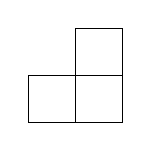
\begin{tikzpicture}[x=0.6cm,y=0.6cm]
\draw (0,0) rectangle (1,1);
\draw (1,0) rectangle (2,1);
\draw (1,1) rectangle (2,2);
\end{tikzpicture}
\end{adjustbox}
\end{center}
\textit{[Справа от рисунка:]} обойдём на плоск. замкн. путь
соотв. путь на кубе: придём в другую точку (кручение)
и повернёмся (кривизна).

Неясно, как на многогранниках выглядят основные геом. вещи
($n$-мерный случай). Хар. классы и т.д.
\textit{[Зачёркнуто:]} …\Incomplete{GELFAND-P000627}{cancelled-geometry}{Зачёркнутое слово после «и т.д.» не восстановлено}
\underline{Задача:} сделать общую теор. относительности на решётках.

\underline{Список того, что нужно знать из физики (разумному математику):}

1. Фейнман, Хибс «Кв. мех. и инт. по траекториям».

2. Лекции Фейнмана для школьников.

3. Квантовая механика: Ландау, Лифшиц (теория возмущ., квазиклассич.
приближение \textit{[Зачёркнуто:]} \Unclear{GELFAND-P000627}{landau-short}{закрывающая скобка / знак};
группы Ли, осн. понятия по теории рассеяния).

4. Релятив. кв. мех. — начало Берестецкий, Лифшиц, Питаевский;
вторичное квантование (кн. Дирака \textit{[Зачёркнуто:]} \Unclear{GELFAND-P000627}{dirac-short}{закрывающая скобка / знак};
Фейнман «Стат. механика»).

Стат. физика — Ландау и Лифшиц.
\SourcePage{GELFAND-P000628}{unlabelled}
\underline{Что надо знать из математики физикам?}

1. Предст. групп.

2. Псевдодифф. операторы.

3. Интегр. опер. Фурье--Хёрмандера.

4. $P^\lambda$ (полиномы Бернштейна).
\begin{equation*}
LP^\lambda=d(\lambda)P^{\lambda-1}.
\end{equation*}
5. Теорема Римана--Роха.

6. Связь особ. с топ. циклов.

\underline{Поляков.}
[Зачёркнута строка; отдельные петли букв видны.]
\Incomplete{GELFAND-P000628}{cancelled-heading}{Зачёркнутая строка под «Поляков» не восстановлена.}
[Справа:] ТМФ предпосл. номер; ст. по полю Янга--Миллса — расписано.

Янг, Миллс — перв. в сб. «Элем. частицы и компенсир. поля» (1964).

Есть кварки $q\simeq\begin{pmatrix}u\\d\\s\end{pmatrix}$.
Спин кварка $1/2$, $B$ — спин $1/2$ (барион), $M$ — спин $0$ (мезон).
\begin{equation*}
M\sim\overline q q\quad(\text{кварк и антикварк}),\qquad B\sim q q q.
\end{equation*}
\underline{Откуда:} Группы в период. системе (по 8 штук).
(Идея Гелл-Манна и Неймана).
$\Rightarrow$ Симметрии: наиболее подх. гр. $SU(3)$, предст. $8,10,27$ (разл.).

Низшие представления?
[Зачёркнут короткий знак: \Unclear{GELFAND-P000628}{reps-short}{U}.]
скалярн., станд. и тенз. произвед.

Пусть это реальные частицы! Замеч. идея:
\begin{equation*}
3^*\times3=1+8,\qquad 3\times3\times3=1+8+8+10.
\end{equation*}
$\Rightarrow$ Нельзя стр. мезоны как 3 кварка; их 8, а $3\times3=3^*+6$.

Рассеиваем:
\begin{equation*}
\frac{\sigma(BB)}{\sigma(BM)}=\frac32\qquad(\text{сечения})
\end{equation*}
— так и получается (точн. $10\%$).

Большие эн. — рассеив. [Зачёркнуто слово; возможное «элем.»]
\Incomplete{GELFAND-P000628}{scatter-cancelled-word}{Зачёркнутое слово перед «частиц» не восстановлено.}
частиц на частице, как част. на античастице.

$q q q q\overline q$ — отсутств. в опыте (наз. экзотическими).

Много частиц — скор. вращ. кварков (как электрон в ат. водорода).
но: нестабильны (резонсы). Перех. в основное состояние.

\underline{Волн. ф-я бариона:}
\begin{equation*}
\Delta^{++}\simeq u(x_1)u(x_2)u(x_3),
\end{equation*}
но функция антисимм.

Предп. 3 сорта и 3 цвета.
\begin{equation*}
q=\begin{pmatrix}
u_{\text{к}}&u_{\text{ж}}&u_{\text{с}}\\
d_{\text{к}}&d_{\text{ж}}&d_{\text{с}}\\
s_{\text{к}}&s_{\text{ж}}&s_{\text{с}}
\end{pmatrix}.
\end{equation*}
[Под столбцами:] красн., жёлт., синие.
[Справа от строк:] верхние, нижние, странные (Гелл-Манн).

На опыте кварки не сущ. ($90\%$).
$\mathcal L$ не может быть инвар. отн.
\begin{equation*}
SU(3)\otimes SU_c(3)\qquad(\text{перемен. цвета}).
\end{equation*}
[Стрелка к $SU_c(3)$:] цветная.
\SourcePage{GELFAND-P000629}{unlabelled}
Счит., что только бесцв. част. имеют не очень большие массы, цветные — $\infty$.
\begin{equation*}
M\sim\overline q_{\text{к}}q_{\text{к}}+
\overline q_{\Unclear{GELFAND-P000629}{meson-index}{\text{жс}}}
\overline q_{\text{жс}}+\overline q_{\text{с}}q_{\text{с}}.
\end{equation*}
[Во втором слагаемом черты стоят над обоими $q$.]
Лагранжиан должен запретить появл. цветных частиц (должны им беск. массы).
Пусть взаимод. перен. цв. полями Янга--Миллса (глюонами).

$SU(3)$ — прибл. симметрия ($20$--$30\%$).
Пусть $SU_c(3)$ — точная группа.
(Возм., есть 4-й сорт (очарованные), но наверняка есть 3 цвета).

Мезонов (см. ф-лу) должно быть 9. Но их больше. Отсюда необх. 4-й кварк.
(4 года назад). [Зачёркнуто; возможное начало «пр…».]
\Incomplete{GELFAND-P000629}{cancelled-quark-line}{Зачёркнутая запись после «4 года назад» не восстановлена.}
[Справа:] $SU(4)\otimes SU_c(3)$.
\begin{equation*}
\mathcal L=\overline q(i\gamma_\mu\nabla_\mu-m)q+
\frac{1}{4e^2}\operatorname{Sp}(F_{\mu\nu}^{,2}).
\end{equation*}
Есть 8 полей Янга--Миллса. (Глюон — от «glu» — клей — склеив. кварки).
Они безмассовые. 8 цветных глюонов.

Сохр. токи $\Longleftrightarrow$ наличие симметрии.
Хотим показать, что если гр. неабелева $\Rightarrow$ эн. взаимод.
$\sim\Unclear{GELFAND-P000629}{cancelled-potential}{[зачёркнутая дробь]}R$ (расст.)
($\Rightarrow$ струна, соед. кварки, не рвётся)
(в абелевой $\sim R^{-1}$, ур-я Максвелла).
\begin{equation*}
\mathcal L=\frac{1}{4e^2}\operatorname{tr}(F_{\mu\nu}^{,2}).
\end{equation*}
\begin{center}
\begin{adjustbox}{max width=\linewidth}
\begin{tikzpicture}[x=1cm,y=1cm]
\filldraw[fill=gray!25] (0,1.8) circle (.18);
\filldraw[fill=gray!25] (0,.2) circle (.18);
\draw (0,.4) .. controls (-.12,.5) and (.12,.6) .. (0,.7)
 .. controls (-.12,.8) and (.12,.9) .. (0,1)
 .. controls (-.12,1.1) and (.12,1.2) .. (0,1.3)
 .. controls (-.12,1.4) and (.12,1.5) .. (0,1.6);
\node[right] at (.35,1) {$M\to\infty$};
\node[right] at (2,1) {2 тяжёлых заряда};
\end{tikzpicture}
\end{adjustbox}
\end{center}
\underline{Г. Класси. вид.: некоммут. электротехника.}
\begin{center}
\begin{adjustbox}{max width=\linewidth}
\begin{tikzpicture}[x=1cm,y=1cm]
\draw (0,1.2) .. controls (.5,1.4) and (1.1,1.2) .. (1.6,1.35);
\draw (0,0) .. controls (.5,.25) and (1.1,.1) .. (1.6,-.15);
\draw (.5,.2) -- (.6,.45) -- (.5,.6) -- (.65,.8) -- (.55,1.3);
\draw (1.05,.12) -- (1.1,.45) -- (1,.6) -- (1.16,.9) -- (1.1,1.28);
\draw[xshift=3cm] (0.118,1.220) .. controls (0.471,0.970) and (1.071,1.090) .. (1.576,1.330);
\draw[xshift=3cm] (-0.047,0.000) .. controls (0.294,0.190) and (0.553,0.150) .. (0.824,0.040) .. controls (1.165,-0.060) and (1.435,-0.190) .. (1.635,-0.160);
\draw[xshift=3cm] (0.541,0.880) .. controls (0.859,0.940) and (1.200,0.880) .. (1.282,0.800) .. controls (1.435,0.620) and (1.035,0.380) .. (0.671,0.500);
\draw[xshift=3cm] (0.471,0.760) .. controls (0.294,0.680) and (0.400,0.580) .. (0.600,0.540);
\draw[xshift=3cm] (0.600,1.080) .. controls (0.494,1.010) and (0.753,1.000) .. (0.694,0.920) -- (0.576,0.790);
\draw[xshift=3cm] (1.071,1.120) .. controls (1.012,1.000) and (1.012,0.970) .. (1.165,0.920);
\draw[xshift=3cm] (0.565,0.460) .. controls (0.447,0.350) and (0.447,0.320) .. (0.600,0.290) .. controls (0.694,0.250) and (0.541,0.170) .. (0.494,0.110);
\draw[xshift=3cm] (0.976,0.460) .. controls (0.906,0.300) and (1.106,0.330) .. (1.235,0.290) .. controls (1.400,0.250) and (1.247,0.160) .. (1.118,0.090);
\draw[xshift=3cm,<-] (1.7,.7) -- (2.1,.7);
\node[xshift=3cm,right,align=left] at (2.1,.7) {обр. пары цв.--антицв.\\(глюонами)};

\end{tikzpicture}
\end{adjustbox}
\end{center}
[Справа от первого малого рисунка:] обмен клеем (глюонами).
\Unclear{GELFAND-P000629}{heavy-note-word}{Малый} вклад, если $M\to\infty$.
\begin{equation*}
\frac{\int DA_\mu\,e^{i\int\mathcal L\,d^4\Unclear{GELFAND-P000629}{action-dx}{x}}
\operatorname{tr}e^{i\oint_C A_\mu dx_\mu}}
{\int DA_\mu\,e^{i\int\mathcal L\,d^4x}}
=\left\langle\operatorname{tr}e^{i\oint_C A_\mu dx_\mu}\right\rangle=e^{iW(C)}.
\end{equation*}
\begin{center}
\begin{adjustbox}{max width=\linewidth}
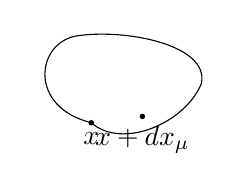
\begin{tikzpicture}[x=1cm,y=1cm]
\draw (0,0) .. controls (-.8,.2) and (-.7,1) .. (-.2,1.1)
 .. controls (.4,1.2) and (1.5,1) .. (1.4,.5)
 .. controls (1.2,0) and (.4,-.35) .. (0,0);
\fill (0,0) circle (.035);\fill (.65,.08) circle (.035);
\node[below] at (0,0) {$x$};\node[below] at (.65,.08) {$x+dx_\mu$};
\end{tikzpicture}
\end{adjustbox}
\end{center}
\begin{equation*}
\operatorname{tr}\prod_x(1+iA_\mu(x)dx_\mu)
\end{equation*}
— контурный интеграл.
(такое упорядочение).
($T$ — экспонента Дайсона).

\underline{Утверждение:}
\begin{center}
\begin{adjustbox}{max width=\linewidth}
\begin{tikzpicture}[x=1cm,y=1cm]
\draw[<->] (-.8,0) -- (4.6,0) node[right] {$\Unclear{GELFAND-P000629}{graph-label}{t}$};
\draw[->] (0,-.3) -- (0,1.6) node[above] {$R$};
\draw (0,0) -- (.7,1) -- (2.8,1) -- (3.6,.05);
\draw (0,-.05) -- (.6,-.8);
\draw (.75,-.85) -- (2.7,-.85);
\draw (2.9,-.7) -- (3.6,-.02);
\draw[<->] (1.55,-.85) -- (1.55,1) node[midway,right] {$R$};
\draw (.7,-.9) -- (.7,-1.45);\draw (2.7,-.9) -- (2.7,-1.45);
\draw[<->] (.7,-1.3) -- (2.7,-1.3) node[midway,below] {$T$};
\node at (3.1,1.3) {$C$};
\end{tikzpicture}
\end{adjustbox}
\end{center}
Рассм. такой контур.
Здесь $W(C)\overset{T\to\infty}{\longrightarrow}E(R)T$, где $E(R)$ — энергия взаимод. зарядов.
\SourcePage{GELFAND-P000630}{unlabelled}
\underline{Объяснение.} если сист. в стац. сост., то амплит. перех.
за время $T$: $F=e^{-iET}$ ($E$ — энергия).
С другой стор. $F=e^{-iET}=\sum e^{iS}$ (пути).
\begin{center}
\begin{adjustbox}{max width=\linewidth}
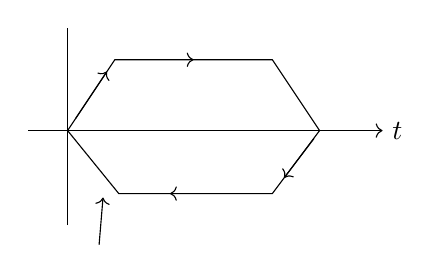
\begin{tikzpicture}[x=1cm,y=1cm]
\draw[->] (-.5,0) -- (4,0) node[right] {$t$};
\draw (0,-1.2) -- (0,1.3);
\draw (0,0) -- (.6,.9) -- (2.6,.9) -- (3.2,0) -- (2.6,-.8) -- (.65,-.8) -- cycle;
\draw[->] (.1,.15) -- (.5,.75);\draw[->] (1,.9) -- (1.6,.9);
\draw[->] (3.13,-.1) -- (2.75,-.6);\draw[->] (1.9,-.8) -- (1.3,-.8);
\draw[->] (.4,-1.45) -- (.45,-.85);
\end{tikzpicture}
\end{adjustbox}
\end{center}
Созд. пары част.--античаст. (сверхтяж.); держим долго.
Класси. действие $S=\int_{(x)}^{(x')}A_\mu dx_\mu$. в эл.-магн. поле.
Античаст. $\sim$ част., идущая назад по времени.
Отсюда $W(C)\sim S_c$ (площадь, внутри контура).
$\sim RT\to E\sim R$.
Считается методом перевалов.
\begin{equation*}
\int DA_\mu\,e^{i\int(\partial_\mu A_\nu-\partial_\nu A_\mu)^2}
e^{i\oint A_\mu dx_\mu}
=e^{-\oint\!\oint dx\,dx' D(x-x')},
\end{equation*}
где $D=\dfrac{1}{(x-x')^2+i0}$ (ф-я Грина ур-я Даламбера).
\begin{equation*}
W=\mathrm{const}\cdot T+\frac{e^2T}{R}+\ldots
\end{equation*}
След. раз:
\begin{equation*}
\frac{\int DA\,e^{\frac{1}{4e^2}\int F_{\mu\nu}^{,2}}
\Unclear{GELFAND-P000630}{cancelled-exponent-atom}{[зачёркнутый знак]}
\cdot\operatorname{tr}e^{\oint A_\mu dx_\mu}}{N}
\end{equation*}
[Под зачёркнутым знаком вставлено: $\cdot\operatorname{tr}e$.]
— вычислим.
Негауссов т.к. в $F_{\mu\nu}$ есть квадр. член $[A_\mu,A_\nu]$.
\begin{equation*}
F_{\mu\nu}=\partial_\mu A_\nu-\partial_\nu A_\mu+[A_\mu,A_\nu].
\end{equation*}
(В эл.-магн. поле коммутатор $0$).
Эл.-дин. с компактной калибр. группой — уже возникает неоднозн. экстремалей.
Кварки в Янге--Миллсе не сделано.
\SourcePage{GELFAND-P000631}{unlabelled}
\underline{9/II-76. Сем. Гельфанда.}
\underline{Кричевер.}
\underline{Ур-\Unclear{GELFAND-P000631}{heading-short}{а} Зах.--Шабата.}
\begin{equation*}
\left[L_1-\frac{\partial}{\partial y},L_2-\frac{\partial}{\partial t}\right]=0,\qquad(1)
\end{equation*}
\begin{equation*}
L_1=\sum_{i=0}^n u_i(x,y,t)\frac{\partial^i}{\partial x^i},\qquad
L_2=\sum_{i=0}^m v_i(x,y,t)\frac{\partial^i}{\partial x^i}.
\end{equation*}
\begin{equation*}
u_n=1,\quad u_{n-1},\quad v_m=1,\quad v_{m-1}\quad\}=\mathrm{const}.
\end{equation*}
[После $u_n$ под $1$ зачёркнуто выражение; ниже виден знак, похожий на $3$.]
\Incomplete{GELFAND-P000631}{coeff-cancelled-expression}{Зачёркнутое выражение в условии на старшие коэффициенты не восстановлено.}

Рассм. форм. ряд
\begin{equation*}
\Psi=e^{kx+k^ny}\left(\sum_{i=0}^{\infty}\xi_i(x,y,t)\frac{1}{k^i}\right),
\qquad \xi_0=1.\qquad(2)
\end{equation*}
Пусть $\left(L-\dfrac{\partial}{\partial y}\right)\Psi=0$, где $L=L_1$.
Коэфф. рекурр. вычисл.
\begin{equation*}
\sum_{i=0}^n u_i\sum_{\ell=0}^i C_i^{\ell}\xi_{\ell-s}^{(i-\ell)}
=\xi_{n-s}+\frac{\partial}{\partial y}\xi_{-s},\qquad
s=n,n-1,\ldots\ \text{до }-\infty.\quad(3)
\end{equation*}
$\xi_{-s}=0$ при $s\Unclear{GELFAND-P000631}{zero-index-range}{>}0$.
[Зачёркнуто слово; возможное «оно» / «ещё».]
\Incomplete{GELFAND-P000631}{cancelled-before-determined}{Зачёркнутое слово перед «опред.» не восстановлено.}
опред. $\xi'_{n-s}$ $\Rightarrow$ надо const интегр.
$\xi_0=1$, $\xi_i(0,y,t)=0$ при $i>1$ — нормировка.
Обр., $\forall$ ряда $\exists$ оп., где всё вып. с точн. до $k^{-1}$.

\underline{Алгебраич. оператор.} — если $\exists$ анал. прод. по $1/k$ на комп.
алг. кривую (мером. в доп. к точке), где сущ. особ.

\underline{Г.} Ур-е Зах.--Шабата
\begin{equation*}
\frac{\partial K_2}{\partial y}-\frac{\partial K_1}{\partial t}=[K_1,K_2],
\end{equation*}
$K_1,K_2$ — дифф. операторы.
$K_1,K_2$ — матр. по $y$ и $t$ или опер. по другим переменным.
Есть много путей, прив. к этому ур-ю.
$y,t$ — параметры.
[Слева зачёркнуто: \Unclear{GELFAND-P000631}{margin-short}{На}.]
Установим равноправие $x,y,t$. Тогда записывается в виде (1).
Зад. для школьников: найти опер. вида
\begin{equation*}
-\frac{d^2}{dx^2}+u(x)=L_1,\qquad
\frac{d^3}{dx^3}+v_1\frac{d}{dx}+v_2=L_2,
\end{equation*}
к-рые коммутируют. Делается через эллипт. ф-и или эллипт. кривые.
Если только $\dfrac{d^n}{dx^n}$, то
\begin{equation*}
\frac{d^n}{dx^n}\Psi-\frac{\partial\Psi}{\partial y}=0
\quad\Rightarrow\quad\Psi=e^{kx+k^ny}.
\end{equation*}
\SourcePage{GELFAND-P000632}{unlabelled}
Точнее: метод интегр. опер. Фурье.
\begin{equation*}
e^{kx+k^ny}\left(1+\frac{\xi_1(x,y,t)}{k}+\ldots\right).
\end{equation*}
\underline{Кр.} Сопост. каждому оп. $L$ — форм. ряд (2).
Рекурр. соотн. (3) однозн. восст. с точн. до нормировки.

\underline{Определение.} $L$ наз. алгебраическим, если форм. ряд (2)
имеет мером. прод. (в доп. к отм. точке) на комп. алг. кривую,
причём полюса не зависят от $x,y,t$.
\begin{equation*}
L\longrightarrow\mathcal R
\end{equation*}
[После стрелки перед $\mathcal R$ зачёркнута запись; видны $\Psi$- и $B$-подобные штрихи.]
\Incomplete{GELFAND-P000632}{curve-cancelled-expression}{Зачёркнутая запись перед обозначением кривой не восстановлена.}
$\mathcal R$ — алг. кр. с отм. точкой $P_0$ и наб. полюсов
$D_1\Unclear{GELFAND-P000632}{polepoints-short}{[зачёркнутый знак]}\ldots+D_g$, $g$ — род кривой
— это наз. данные рассеяния для $L$.
$P_0$ — точка, где сущ. особ.
$1/k$ — лок. парам. в окр. $P_0$.

\underline{Г.} Асимпт. разл. как правило не сходится.
В опр. предпол. сходимость.
\underline{К.} Алг. оператору $L\longrightarrow$ алг. крив. с отм. точкой и набор полюсов.
\underline{Г.} $C^\infty$ — ф-ла Тейлора асимпт. $\Rightarrow$ аналит. — сход.
Аналог квазианалитичности?

\underline{К. Т. (Ахиезер)} $\forall$ неособ. алг. кривой $\mathcal R$ с отм. точкой $P_0$
и фикс. лок. пар. в окр. $P_0$ и отм. наб. полюсов
$\exists$ однозн. опр. с точн. до проп. ф-я $\Psi(x,y,P)$ с зад. наб. полюсов и
\begin{equation*}
\underbrace{\Psi(x,y,P)e^{-kx-k^ny}}_{1+o(1/k)}
\quad\text{— рег. в окр. }P_0.
\end{equation*}
\begin{center}
\begin{adjustbox}{max width=\linewidth}
\begin{tikzpicture}[x=1cm,y=1cm]
\draw (0,0) rectangle (1.2,.8);
\end{tikzpicture}
\end{adjustbox}
\end{center}
$e^{\zeta(P)x}$ [стрелка к $\zeta$:] Вейерштрасса (Камке).
\underline{Д-во:} явная ф-ла (будет предъявлена позже).
\underline{Теор.} Ур-е алгебраично $\Rightarrow\exists$ ф-я $\Psi\Rightarrow$ мы знаем все $\xi$
$\Rightarrow$ находятся все $u_i$ (однозн.) — почему они сущ.?
По \Unclear{GELFAND-P000632}{bottom-short}{[зачёркнутый знак]} $\Psi$ находятся $u_i$!!
[Внизу справа зачёркнуто: $\forall$ ряда $\exists$ опер.; ниже виден фрагмент «р…».]
\Incomplete{GELFAND-P000632}{bottom-cancelled-insert}{Короткая запись под левым концом зачёркнутой строки не восстановлена.}


\SourcePage{GELFAND-P000633}{unlabelled}
$\forall$ рода $\exists$ опер.:
\begin{equation*}
L\psi-\frac{\partial}{\partial y}\psi=
\text{[зачёркнуто: \text{\Unclear{GELFAND-P000633}{top-cancel}{$\psi$}}]}
(e^{kx+k^ny}O(\text{\Unclear{GELFAND-P000633}{top-o-argument}{$\frac{1}{k}$}})).
\end{equation*}
(первые $n-2$ ур-я)

$L\psi-\frac{\partial\psi}{\partial y}$ уд. всем треб. теор. Ахиезера
$\Rightarrow$ она $\equiv0$.

\underline{Дринфельд.}

\underline{Попытка алгебраизации прошлого докл. Кричевера}

Опис. коммут. подколец в кольце дифф. операторов.

\underline{Г.} Цель — некот. законы взаимности.

$B-$ [зачёркнутое слово:] \Incomplete{GELFAND-P000633}{b-first-cancel}{Зачёркнутое слово после $B-$ неразборчиво.}, комм. кольцо с $1$, снабж. дифф.
[зачёркнуто: \Unclear{GELFAND-P000633}{b-derivative-cancel}{$\delta$}] $b\mapsto b'$ [зачёркнуто: \Unclear{GELFAND-P000633}{b-prime-cancel}{$\xi$}].
($\mathbb C$-алгебра)

\begin{equation*}
B[D],\qquad \sum b_iD^i\quad\text{(многочл.)},\qquad
\underbrace{Db-bD=b'}_{\text{прав. умножения}}.
\end{equation*}
($b'$ — произв. в $B$)

$X$ — комп. рим. пов. над $\mathbb C$, $P$ — фикс. точка. Обозначим
через $A$ кольцо мером. ф-й на $X$ [зачёркнутое слово:] \Incomplete{GELFAND-P000633}{a-poles-cancel}{Зачёркнутое слово после $X$ неразборчиво.}
с полюсом лишь в $P$.

Опишем гомоморфизмы $A\to B[D]$.

(на самом деле других комм. подколец не бывает — теор. Шабата)

\underline{Г.} Реальная зад.: найти все расширения тел Гельфанда-Кириллова.

Полиномиальность мешает.

\begin{equation*}
\sum_{i=0}^k b_iD^i,\qquad \underline{\text{эллиптичность}}:\quad\exists b_k^{-1}.
\end{equation*}
\underline{Треб.:} образ $\forall$ ненулев. элем. из $A$ эллиптичен.

\underline{Ранг.} $a\ne0$, $a\in A$.

$\operatorname{ord}(a)$ — порядок образа $a$.
\begin{align*}
\operatorname{ord}(ab)&=\operatorname{ord}(a)+\operatorname{ord}(b),\\
\operatorname{ord}(a+b)&\le \text{[зачёркнуто: \text{\Unclear{GELFAND-P000633}{norm-cancel}{$\operatorname{ord}(a)+\operatorname{ord}(b)$}}]}
\max(\operatorname{ord}(a),\operatorname{ord}(b)),\\
\operatorname{ord}\lambda&=0\quad\text{при }\lambda\in\mathbb C.
\end{align*}
[Справа общая скобка: \underline{нормирование}.]

$\operatorname{deg}a$ — порядок полюса $a$ в точке $P$.

\underline{Тогда} $\underline{\operatorname{ord}(a)=n\operatorname{deg}(a)}$.
(на многочленах — ясно)

$n$ — ранг гомоморфизма.

\underline{Кричевер} — $n=1$ (вз. простота порядков опер.)

$M=B[D]$, на $M$ есть структ. $B$-модуля;
$\varphi:A\to B[D]$.
\SourcePage{GELFAND-P000634}{unlabelled}
$M_n$ — опер. порядка $\le n$.

[Зачёркнуто: \Unclear{GELFAND-P000634}{top-cancel}{Это} $B$-модуль.]

$M$ — это $A\otimes B$-модуль, т.е. $A$-модуль и $B$-модуль и
умн. на $A$ и $B$ коммутируют.
\begin{align*}
bx&=bx\quad\text{(умн. слева)},\\
ax&=x\varphi(a),\\
a\in A&\Rightarrow aM_i\subset M_{i+\operatorname{deg}a\cdot n}.
\end{align*}
$\nabla:M\to M$ — умн. слева на $D$,
$\nabla(x)=Dx$.

$\nabla$ коммут. с действ. $A$, а $\nabla b-b\nabla=b'$.

\underline{Обр.} если есть $A\otimes B$-мод. $M$ с фильтр. и всеми этими
соотн., то $\exists$ гомом. $\varphi:A\to B[D]$ ранга $n$.

Можно забыть о $\varphi$ и рассм. зад. об $A\otimes B$-модулях.

Итак, $M$ — модуль над $A\otimes B$, снабж. [зачёркнуто:] \Incomplete{GELFAND-P000634}{filtration-cancel}{Зачёркнутое слово перед «фильтрацией» неразборчиво.} фильтрацией
\begin{equation*}
0=M_{-1}\subset M_0\subset M_1\subset M_2\subset\cdots
\end{equation*}
[$A$: мером. ф-и на $X$ с ед. полюсом. $B$: кольцо ($\mathbb C$-лин.)
с дифф. $b\mapsto b'$.]

и оператором $\nabla:M\to M$, причем

1) $\nabla a=a\nabla$;

2) $\nabla b-b\nabla=b'$;

3) $\nabla(M_i)\subset M_{i+1}$,
$\nabla:M_i/M_{i-1}\overset{\sim}{\to}M_{i+1}/M_i$ при $i\ge0$.

4) $bM_i\subset M_i$, $M_i/M_{i-1}$ [зачёркнуто: \Unclear{GELFAND-P000634}{condition-four-cancel}{$\to$}]
своб. $B$-модуль с $1$-й образующей.

5) $aM_i\subset M_{i+n\operatorname{deg}a}$,
$a:M_i/M_{i-1}\overset{\sim}{\to}
M_{i+n\operatorname{deg}a}/M_{i+n\operatorname{deg}a-1}$ при $i\ge0$.

$\sim$ зад. пучка над $X\otimes B$ с нек-рыми фильтрациями.

$\nabla\sim$ связность с особ. на $\infty$.
[Внизу горизонтальные черты, между ними точка.]
\SourcePage{GELFAND-P000635}{unlabelled}
\underline{23/II-76.}\quad \underline{Сем. Гельфанда.}

\underline{С.П. Новиков} о раб. М. Бродского. (Минск)

\underline{Нек-рые случаи явно решаемых зад., не связ. с KdV.}

\underline{Зад. о колеб. упругого шара.}
\begin{equation*}
-\frac{d^2y}{dr^2}+\left(\lambda^2f^2(r)-\frac{\ell(\ell+1)}{r^2}\right)y
=\lambda_{k,\ell}y.
\end{equation*}
Обр. зад. — вост. пар. упр. среды по набору частот $\lambda_{k,\ell}$.

Задача переопред. Вычисл., когда реш. и как.

Пусть $rf(r)=u(r)$ монотонная ф-я.

Рассм.
\begin{equation*}
m(\tau)=\int_{H(\tau)}^1\left(\tau^{-2}f^2(r)-\frac1{r^2}\right)^{1/2}dr
\quad\text{(прав. квант. Бора)}.
\end{equation*}
($H(\tau)$ — нуль подкор. выражения)

Рассм.
\begin{equation*}
\tau^*_{k\ell}=\frac{\sqrt{\ell(\ell+1)}}{\lambda_{k\ell}},\qquad
m_{k\ell}=\frac{k+1/4+C}{\sqrt{\ell(\ell+1)}}.
\end{equation*}
$\tau^*(m_{k\ell})=\tau^*_{k\ell}$ уст. вз.-однозн. соотв.

$m_{k\ell}$ всюду плотно;
необх. усл. — $\tau_{k\ell}$ плотно.

$(rf(r))^{-1}=\psi(\eta)$;\qquad $\tau(m)\leftarrow m(\tau)$.
\begin{equation*}
\psi(\eta)=\exp(2\int^1(\tau^2-\eta^2)^{-1/2}
\frac{d(\tau m(\tau))}{d\tau}d\tau
\end{equation*}
Большие $\ell$ — квазиклассика.

\underline{Фукс.} Есть мн-зия триангул.
\begin{center}
\begin{adjustbox}{max width=\linewidth}
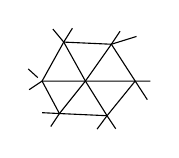
\begin{tikzpicture}[scale=0.55]
\draw (-1,0)--(-.5,.9)--(.6,.85)--(1.15,0)--(.5,-.8)--(-.6,-.75)--cycle;
\draw (-1.3,-.2)--(-1,0)--(0,0)--(1.5,0);
\draw (-.75,1.2)--(-.5,.9)--(0,0)--(.5,-.8)--(.7,-1.1);
\draw (.8,1.15)--(.6,.85)--(0,0)--(-.6,-.75)--(-.8,-1.05);
\draw (-.5,.9)--(-.3,1.22);
\draw (.6,.85)--(1.18,1.03);
\draw (1.15,0)--(1.43,-.43);
\draw (.5,-.8)--(.27,-1.11);
\draw (-.6,-.75)--(-1,-.73);
\draw (-1.32,.28)--(-1.1,.08);
\end{tikzpicture}
\end{adjustbox}
\end{center}
Рассм. $\sum$ всех симпл. $1$-й разм. с коэфф. $1\bmod2$. Она не цикл.

У $1$-го барицентр. подразделения $0$.
\begin{center}
\begin{adjustbox}{max width=\linewidth}
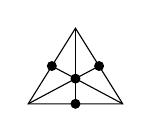
\begin{tikzpicture}[scale=0.6]
\draw (0,1.6)--(-1,0)--(1,0)--cycle;
\draw (0,1.6)--(0,0);
\draw (-1,0)--(.5,.8);
\draw (1,0)--(-.5,.8);
\fill (0,.533) circle (3pt);
\fill (0,0) circle (3pt);
\fill (-.5,.8) circle (3pt);
\fill (.5,.8) circle (3pt);
\end{tikzpicture}
\end{adjustbox}
\end{center}
\underline{все центры}, $\underline{0\bmod2}$ (чётное).

\underline{Штиф. класса} — ему двойственен по Пуанкаре.

$\sum$ числа $=\sum(-1)^i$ чисел $\bmod2=$ эйл. хар.

\underline{Лосик (Марк).}

\underline{Связность.} $E\to X$ векторное расслоение со слоем $\mathbb R^n$;
$p:P\to X$ ассоц. главное расслоение.

$x\in X$, $E_x$ — слой $E$ в т. $x$.

$P_x\ni z$, $z=(e_{i,x})$, $i=1,\ldots,n$, $z$ — базис в $E_x$.

Рассмотрим $G=GL(n,\mathbb R)$ и определим её действие на $P$.
\begin{equation*}
A\in G\rightsquigarrow R_A:P\to P,\qquad
R_A(z)=zA=\left(\sum_{j=1}^ne_{j,x}A_i^j\right),\quad
A=(A_i^j),\quad i,j=1,\ldots,n.
\end{equation*}
Это действие гладкое.
\SourcePage{GELFAND-P000636}{unlabelled}
1. $(zA)B=z(AB)$.

2. $G$ сохр. слои и действ. просто транзитивно.

$z\in P_x$, $V_z$ — вертик. кас. пр-во ($\subset T_zP$);
$V_z=T_z(P_x)$.

опред. отобр. $\ell_z:G\to P_x$, $\ell_z(A)=zA$

и индуц. отобр.
$\alpha_z:T_e(G)=\mathfrak g\to V_z$ (изоморфизм).

$\beta_z=\alpha_z^{-1}:V_z\to\mathfrak g$.
(лин. форма на $V_z$ со знач. в $\mathfrak g$).

\underline{Связность на гл. расслоении} — $1$-форма на $P$ со знач. в $\mathfrak g$,
такая, что

1. $\omega|_{V_z}=\beta_z$;

2. $R_A^*\omega=\operatorname{ad}A^{-1}\omega$ (усл. инвариантности).

Для кас. рассл. — аффинная связность.

Рассм. ур-е $\omega=0$ в т. $z$;
$H_z=\{\xi\in T_zP:\omega(\xi)=0\}$.

$H_z$ наз. горизонтальным пр-вом.

$T_z=H_z\oplus V_z$.

$H_z$ сохр. при действии $G$.

Будет постр. рассл., сечение к-рого нах. во вз.-одн. соотв. со связн. на $P$.

Рассмотрим $T_z^*\otimes\mathfrak g$ — $1$-формы в т. $z$ со знач. в $\mathfrak g$.

Опр. $\Theta_z\subset T_z^*\otimes\mathfrak g$ как подпр. тех $\theta_z$, что
$\theta_z|_{V_z}=0$.

$C_z\subset T_z^*\otimes\mathfrak g$, $C_z\ni\omega_z:\omega_z|_{V_z}=\beta_z$.

$C_z-C_z\subset\Theta_z$,\quad $\omega_{1,z}-\omega_{2,z}\in\Theta_z$,
\quad $\omega_z+\Theta_z\subset C_z$.

т.е. $C_z$ — плоскость, паралл. $\Theta_z$, но не прох. через $0$.

Получается рассл. из аффинных пр-в
(«разн. $2$-х симв. Кристоффеля — тензор»).

Над $P$ рассм. рассл. со слоем $T_z^*\otimes\mathfrak g$.

Есть отображения:
$\widetilde r_{z,A}:T_z^*\otimes\mathfrak g\to T_{zA}^*\otimes\mathfrak g$,
индуцир. отображением

$R_{A^{-1}}^*:T_z^*\to T_{zA}^*$ и
$\operatorname{ad}A^{-1}:\mathfrak g\to\mathfrak g$.
[Справа: Тенз. произведение отображений.]
\SourcePage{GELFAND-P000637}{unlabelled}
$C_z$ перех. в соотв. плоск. в т. $zA$ при этом отобр.

$C(P)=\bigcup_{z\in P}C_z$ — естеств. гладкое рассл. над $P$.

$G$ действует на $C(P)$.

[Зачёркнуто: \Unclear{GELFAND-P000637}{first-cancel}{$C$}] Инвариантные сечения $\longleftrightarrow$ связности.

\underline{$C(P)/G=B(P)$}, [вставлено и обведено: расслоение, со стрелкой к $\pi$]
$\pi:B(P)\to X$.

\Incomplete{GELFAND-P000637}{quotient-cancel}{Прежняя зачёркнутая надпись под «расслоение» неразборчива.}

$C(P)$ — главное рассл. с базой $P$; там есть кан. связность.

\underline{Габриэлов.}

[Зачёркнуто: Связность \Unclear{GELFAND-P000637}{gabrielov-symbol}{$\zeta$} задается изоморфизмом
$T^*X\otimes\mathfrak g\to B(P)$.]

(на $\forall$ слое — афф. преобразование)

$1$ св. выбр. $\to$ другой св. опр. преобр. исх. пр-ва.

($\Longleftrightarrow$ разн. связностей — тензор)

\begin{adjustbox}{max width=\linewidth}
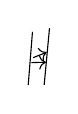
\begin{tikzpicture}[scale=0.45]
\draw (0,0)--(.12,1.5);\draw (.45,0)--(.6,1.6);
\draw[->] (.09,.63)--(.5,.64);\draw[->] (.14,.77)--(.52,.92);
\end{tikzpicture}
\end{adjustbox}

$\lambda\in T_xX\rightsquigarrow E_x\to E_x$

т.е. форма со знач. в гомом.

\underline{$T^*X\otimes\operatorname{Hom}(E,E)$}.

[Горизонтальные черты, между ними точка. Нижняя половина листа пуста.]
\SourcePage{GELFAND-P000638}{unlabelled}
\underline{1/III-76.}\quad \underline{Сем. Гельфанда.}
[Под заголовком прямоугольник с наклонной штриховкой.]

\underline{Дринфельд.} (Володя).

$\overline X$ — гл. проект. кривая над $\mathbb C$,
$P$ — фикс. точка на $\overline X$,

$A\sim$ кольцо рац. ф-й на $\overline X$ с полюсом в $P$
(рег. в $\overline X\setminus P$).

\Incomplete{GELFAND-P000638}{first-cancel}{Зачёркнутое слово после определения $A$ неразборчиво.}

\underline{Г. Пример.} $y^2=x(x-1)(x-2)$ (эллиптическая кривая).

$P=\infty$,\quad $A=\mathbb C[x,y]/(y^2-x(x-1)(x-2))$.

\underline{Ф-и с полюсом $1$-го порядка нет} — т.к. \Incomplete{GELFAND-P000638}{torus-cancel}{Зачёркнутое слово перед «это тор» неразборчиво.} это тор;

два контр.

\begin{adjustbox}{max width=\linewidth}
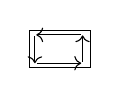
\begin{tikzpicture}[scale=0.6]
\draw (0,0) rectangle (1.3,.8);
\draw[->] (1.1,.7)--(.15,.7);
\draw[->] (.12,.67)--(.12,.1);
\draw[->] (.16,.1)--(1.1,.1);
\draw[->] (1.13,.13)--(1.13,.69);
\end{tikzpicture}
\end{adjustbox}
\quad $\underline{\int=0}$,\quad \underline{вычет $=0$}.

Полюс $2$-го пор. — $\mathcal P$-ф-я Вейерштрасса
(см. Гурвиц, Курант).

\Incomplete{GELFAND-P000638}{genus-zero-cancel}{Зачёркнутое слово перед $y^2=x(x-1)$ неразборчиво.} $y^2=x(x-1)$ рода $0$ — \underline{подст. Эйлера}.

$A$ для крив. рода $0$ — многочлены, обр. $z$.

\underline{$A$ для элл. кривой} — $\mathbb C[x,y]/(y^2-(x(x-1)(x-2))$.

$x$ им. полюс $2$-го пор.; перех. в ф-ю Вейерштрасса
$x=\wp(z)$, $y=\wp'(z)$.

$y$ [знаки повтора] $3$-го пор.

Кольцо $A$ однозн. опр. кривую и точку.

Как опис. эти кольца?

[Горизонтальные черты, между ними точка.]

\underline{Кричевер:} почти $\forall$ точки $P$ наим. пор. полюса $g+1$.

\underline{Иногда можно ниже} — в точках Вейерштрасса.

$y^2=\prod_{i=1}^{2g+1}(z-z_i)$ (гиперэллипт. кривая) —
в т. ветвления есть ф-я с полюсом $2$-го порядка.

$n$ — мин. возм. кр. полюса в т. $P$
$\Rightarrow$ есть полюсы кр. $2n$, $3n$, $\ldots$

Пусть $\mu_s$ такие, что $\mu_s n+s$ — кратность полюса,
$s=1,\ldots,n-1$.

($\mu_s$ — наименьшие).

Тогда $\underline{\mu_1+\cdots+\mu_{n-1}=g}$.
\quad $\Vert$ Среди них все образ. (теор. Вейерштрасса).
\SourcePage{GELFAND-P000639}{unlabelled}
$P$ общ. полож. — кольцо $A$ имеет $g$ образующих —
с полюсами $\underline{g+1,g+2,\ldots,2g+1\text{ порядка}}$.

$B$ — алгебра над $\mathbb C$ с дифференцированием $D$.

Есть кольцо $B[D]=\{\sum b_iD^i\}$, $Db-bD=b'$.

Элем. наз. эллипт., если старш. коэфф. обратим.

Опишем гом. $A\to B[D]$, что образ $\forall$ элем. эллиптичен.

Ранг такого гомоморфизма — число (нат.) $n$, такое что

$\forall a\in A$, $\operatorname{ord}\varphi(a)=n\cdot\operatorname{deg}a$.

$\operatorname{deg}a$ — пор. полюса $a$ \Incomplete{GELFAND-P000639}{degree-cancel}{Зачёркнутое слово после $a$ неразборчиво.} в т. $P$.

(\underline{Г.} Есть дифф. опер. $2$-го и $3$-го пор., коммутир. между собой.)

[Зачёркнуто: \Unclear{GELFAND-P000639}{module-cancel}{$M$}] гомом. $\longleftrightarrow$ модули с доп. структурами.

\underline{Теор. Кричевера.}

Старший коэффициент гомоморфизма $\varphi:A\to B[D]$.

Пусть $z$ — лок. координата в т. $P$. Пусть $a=z^{-k}+\cdots$ (Лорана).

[Зачёркнуто: \Unclear{GELFAND-P000639}{leading-cancel}{Стар}] $\varphi(a)=b^kD^{nk}+\cdots$,

где $\underset{\substack{\uparrow\\B}}{b}$ не зависит от $k$ и от выбора лок. параметра.

(сущ. полюса $\forall$ пор., начиная с нек-рого; надо делить)

\underline{$b$ наз. старшим коэфф. гомоморфизма $\varphi$}.

[Зачёркнуто: \Unclear{GELFAND-P000639}{equivalence-cancel}{Это}] \underline{опр.} $\varphi_1\sim\varphi_2$, если
$\exists b\in B^*$, $\underline{\varphi_1(a)=b\varphi_2(a)b^{-1}}$.

$\dfrac{d}{dx}\sim\dfrac{b'}{b}+\dfrac{d}{dx}$.
В ростках $b'/b$ — любая ф-я.

\underline{Теор. Кричевера.} $B$ \Incomplete{GELFAND-P000639}{germs-formula-cancel}{Зачёркнутая формула после $B$ неразборчива.} — ростки гладких ф-ий на прямой.

гомом. $\varphi$ ранга $1$ (с точн. до эквив!)
$\longleftrightarrow$ старший коэфф. и точка на якобиане кривой
(якобиево многообразие), $J_X$.

\underline{С. Гельф.} \underline{$1$-мерные вект. рассл. степени $0$}
($\sim$ дивизор с точн. до эквивал.)

$Q_1,\ldots,Q_\ell$;
$n_1,\ldots,n_\ell$ [приписано: целые]; степень $n_1+\cdots+n_\ell=0$.

\underline{эквивалентность:} если отлич. на дивизор ф-и (мероморфной)

\underline{Эквив.} — рассл. зад. глоб. мером. сечениями.
\SourcePage{GELFAND-P000640}{unlabelled}
\underline{Г. Аналит. опред. якобиева мн-зия:} на $\overline X$ сущ. дифф. $1$-го рода
(без особ.) их $g$ штук.

$y^2=x(x-a)(x-b)$,

$\Vert\dfrac{dx}{y}$ не имеет особ.
(в т. $x=0,a,b$ нет, т.к. $x$ не лок. парам.)

\begin{adjustbox}{max width=\linewidth}
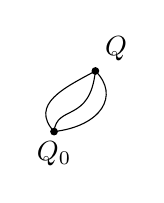
\begin{tikzpicture}[scale=0.7]
\draw (0,0).. controls (-.45,.5) and (.2,.8)..(.75,1.1)
..controls (1.2,.65) and (.85,.1)..(0,0);
\draw (0,0)..controls (.05,.5) and (.65,.15)..(.75,1.1);
\fill (0,0) circle (2pt) node[below] {$Q_0$};
\fill (.75,1.1) circle (2pt) node[above right] {$Q$};
\end{tikzpicture}
\end{adjustbox}

$z_i=\int_{Q_0}^{Q}\omega_i:$ \Incomplete{GELFAND-P000640}{integral-cancel}{Зачёркнутая надпись после интеграла неразборчива.}
($\int$ по кл. гомологий; базис — $g$ чисел)

форма опр. наб. инт. по периодам. $n_1\alpha_1+\cdots+n_{2g}\alpha_{2g}$.

с точн. до периодов — $\mathbb C^g/\underline{\text{решётка}}$.

Не все торы получаются.

Дивизор — лин. комб. точек; точки тора можно склад.

\begin{adjustbox}{max width=\linewidth}
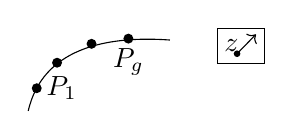
\begin{tikzpicture}[scale=0.6]
\draw (0,0)..controls (.3,1.3) and (1.6,1.6)..(3,1.5);
\fill (.18,.48) circle (3pt) node[right] {$P_1$};
\fill (.61,1.02) circle (3pt);
\fill (1.34,1.42) circle (3pt);
\fill (2.12,1.53) circle (3pt) node[below] {$P_g$};
\draw (4,1) rectangle (5,1.75);
\node at (4.3,1.38) {$z$};\fill (4.42,1.21) circle (2pt);\draw[->] (4.42,1.21)--(4.82,1.62);
\end{tikzpicture}
\end{adjustbox}

движ. по прямой на торе $\to$ движ. $P_1,\ldots,P_g$
\Incomplete{GELFAND-P000640}{motion-cancel}{Зачёркнутое слово перед «по кривой» неразборчиво.} по кривой.

Зад. гом. из $A$ в кольцо $B[D]$ экв. зад. следующего:

$M$ — модуль над $A\otimes B$;
$\nabla:M\to M$, $\nabla(am)=a\nabla(m)$,

$\nabla(bm)=b\nabla(m)+b'm$.

$0=M_{-1}\subset M_0\subset M_1\subset M_2\subset\cdots$,
$\dim_B M_i/M_{i+1}=1$ при $i\ge0$.

$BM_i\subset M_i$;

$\nabla M_i\subset M_{i+1}$,
$\nabla_*:M_i/M_{i-1}\overset{\sim}{\to}M_{i+1}/M_i$.

$aM_i\subset M_{i+\operatorname{deg}a}$,

$a:M_i/M_{i-1}\overset{\sim}{\to}
M_{i+\operatorname{deg}a}/M_{i+\operatorname{deg}a-1}$.

[Горизонтальная черта.]

\underline{$\varphi:A\to B[D]$} $\Rightarrow B[D]=M$.

\Incomplete{GELFAND-P000640}{module-phrase-cancel}{Зачёркнутая фраза под $B[D]=M$ неразборчива.}

Умн. на $B$ слева и на $A$ справа,
$ma\underset{\mathrm{def}}=m\varphi(a)$,
$bm=bm$.

$\nabla:M\to M$ умн. на $D$ слева.

\underline{Фильтр. — порядок.}

\underline{посл. усл. — эллиптичность.}

[Горизонтальные черты, между ними точка.]

Как по $M$ построить $\varphi$?

[Зачёркнуто: \Unclear{GELFAND-P000640}{m-cancel}{$M$}] $M_{-1}=0$;

$\nabla:M_0\overset{\sim}{\to}M_1/M_0$;
в $M_0$ есть образующая $e$ (над $B$).

положим $D=\nabla(e)$.

$\varphi(a)$ ясно, т.к. есть $A$-модуль и т.д.

[Горизонтальные черты, между ними точка.]

\underline{След. шаг:} перев. на язык пучков.

[Зачёркнуто: \Unclear{GELFAND-P000640}{curve-cancel}{на кривой}] $M_{-1}=0\subset M_0\subset M_1\subset\cdots$

(1-мерное) $\sim$ вект. рассл. на $\overline X$ с тривиальн.
$0$ когом. (0-мерн. и 1-мерн.) пучка сечений.

[Справа:] $aM_i\subset M_{i+\operatorname{deg}a}$,
$a:M_i/M_{i-1}\overset{\sim}{\to}M_{i+\operatorname{deg}a-1}$ ($i\ge0$).
\SourcePage{GELFAND-P000641}{unlabelled}
\SourceFigure{GELFAND-P000641}{top-margin-mark}{В правом верхнем поле трёхсторонняя прямоугольная метка; ниже петля и короткие горизонтальные штрихи.}
$L$ — $1$-мерное вект. расслоение над $\overline X$,
$H^0(X,L)=H^1(X,L)=0$.

($H^0(X,L)=0$ и $\operatorname{deg}L=g-1$).

$M=H^0(X-P,L)$ (алгебраические сеч.; гладк. с ед. полюсом).

$M_i$ [зачёркнуто: \Unclear{GELFAND-P000641}{m-i-cancel}{$-$}] с полюсом порядка $i+1$.

$M_{-1}=0$ — $1$-е условие, ($H^0=0$).

$\dim M_i/M_{i-1}=1$,
$M_0=H^0(X,\underset{\substack{\uparrow\\\text{с полюсом в }P}}{L(P)})$.

$0\to L\to L(P)\to L(P)/L\to0$.

точн. посл. когом. $\Rightarrow\dim_{\mathbb C}M_i/M_{i-1}=1$.

[Две горизонтальные черты.]

Обр.: есть послед. модулей, постр. пучок

$0=M_{-1}\subset M_0\subset M_1\subset M_2\subset\cdots$,
$\dim_{\mathbb C}M_i/M_{i-1}=1$.

$M$ — модуль над $A$.

$aM_i\subset M_{i+\operatorname{deg}a}$;

$a:M_i/M_{i-1}\overset{\sim}{\to}
M_{i+\operatorname{deg}a}/M_{i+\operatorname{deg}a-1}$, $i\ge0$.

\underline{Сеч. пучка зададим над откр. мн-вами по Зарискому.}

Пучок квазикогерентный; дост. зад. на откр. афф. подмн-вах.

$a_0\in A$, $a_0\ne\mathrm{const}$
$\Vert$ покрытие $X=(\overline X\setminus P)\cup(\overline X\setminus\text{нули }a_0)$.

Сеч. над $\overline X\setminus P$, $A$-модуль — $M$.

Над $\overline X\setminus\text{нули }a_0$ — $m/a_0^k$,
$m\in M_{k\cdot\operatorname{deg}a_0-1}$.

\underline{След. раз:} Дринфельд $20$ мин., Шнирельман.

\Incomplete{GELFAND-P000641}{bottom-clipped}{Нижняя строка сохранилась только верхушками штрихов; написанное содержание неразборчиво.}
\SourcePage{GELFAND-P000642}{unlabelled}
[Над заголовком горизонтальные черты, между ними точка; слева отдельная точка.]
\underline{15/III-76 г.}\quad \underline{Сем. Гельфанда.}\quad \underline{Дринфельд.}

$\overline X$ — гладкая проект. кривая над $\mathbb C$,

$P\in\overline X$,

$A\in H^0(X-P,\mathcal O_X)$ — рац. ф-и на $\overline X$ с полюсом в $P$.

$B$ — алгебра над $\mathbb C$ (в диффер. [вставлено ниже: опер.]);
$z$ — лок. коорд. на $\overline X$ в окр. $P$.

Ищутся гомоморфизмы $\varphi:A\to B[D]$ ранга $1$,

т.е. $\forall a\in A$, $a=z^{-m}+\cdots\Rightarrow\varphi(a)=b^mD^m+\cdots$;

$b$ — старший коэффициент $\varphi$.

Они рассм. с точн. до сопряжения обрат. элементами из $B$.

[Зачёркнуто: \Unclear{GELFAND-P000642}{assignment-cancel}{$B$}] Задание $\varphi$ равносильно тогда заданию
$A\otimes B$-модуля $M$

[Зачёркнуто: \Unclear{GELFAND-P000642}{first-cancel}{е}] и отображения $\nabla:M\to M$, таких что

$\nabla(am)=a\nabla(m)$, [зачёркнуто: \Unclear{GELFAND-P000642}{am-cancel}{и}]
$\nabla(bm)=b\nabla(m)+b'm$,

$M=\bigcup M_i$ (фильтрация),

$BM_i\subset M_i$, [зачёркнуто: \Unclear{GELFAND-P000642}{bm-cancel}{$BM_i$}]
$M_{-1}=0$, $M_i/M_{i-1}=B$ при $i\ge0$.

$\forall a\in A$, $aM_i\subset M_{i+\operatorname{deg}a}$,
$a:M_i/M_{i-1}\overset{\sim}{\to}M_{i+\operatorname{deg}a}/M_{i+\operatorname{deg}a-1}$.

$\nabla:M_i/M_{i-1}\overset{\sim}{\to}M_{i+1}/M_i$, $i\ge0$.

\underline{Г. следствие:} $\exists$ опер., все степени к-рого, кроме $1$-й —
дифф. операторы ($2$-я, $3$-я и т.д.)

$\overline X$ — алг. кр. рода $g$, $P$ — точка.

$n$ — мин. возм. кратность полюса в т. $P$ (единств. полюса).

$\mu_i$ — наим. числа, для к-рых сущ. полюс кр. $i+\mu_i n$,
$i=1,\ldots,n-1$.

Тогда $\sum\mu_i=g$.


\SourcePage{GELFAND-P000643}{unlabelled}
\Incomplete{GELFAND-P000643}{cancel-top}{[Зачёркнутая фраза: С…; остальное неразборчиво.]}
(Пропущено $g$ кратностей полюсов) [Звёздочка и стрелка к замечанию справа.]
[Стрелка к замечанию:] это [зачёркнуто] и обратно влечёт утв., сформ. Кричевером.
\Incomplete{GELFAND-P000643}{cancel-top-right}{[Зачёркнутое слово после «это» неразборчиво.]}

\underline{Д. На язык пучков.}
Всё, кроме $\nabla$, $\sim$ зад. вект. рассл. $L$ на $X$, для к-рого
$H^0(X,\underline L)=H^1(X,\underline L)=0$.
$\sim$ зад. 1-мерн. рассл. над $X\otimes B$:
$H^0(X\otimes B,\underline L)=H^1(X\otimes B,\underline L)=0$.
\begin{equation*}
X=U_1\cup\ldots\cup U_k,\qquad U_i=\operatorname{Spec}R_i.
\end{equation*}
Склеим афф. схемы $\operatorname{Spec}$ [зачёркнуто] $R_i\otimes B$.
\Incomplete{GELFAND-P000643}{cancel-affine}{[Зачёркнутое выражение после Spec неразборчиво.]}
\underline{Интуитивно:} росток гладк. сем-ва вект. расслоений.
\begin{equation*}
\nabla:\underline L\longrightarrow\underline L(P),\qquad
\underline L\longrightarrow\underline L(P)/\underline L\longrightarrow0.
\end{equation*}
[Стрелка к $L(P)$:] с особ. 1-го пор. в т. $P$.
$H^0(\underline L(P)/\underline L)$ свободно (огранич. на т. $P$ тривиально).
\begin{equation*}
\nabla b-b\nabla=b',\qquad \nabla\quad O_X\text{-линейно}.
\end{equation*}
\underline{Старш. коэфф. --- ?}
Тривиализуем в окр. $P$, пусть $e$ --- базис.
\begin{equation*}
\frac{\nabla(e)}e=\frac1{b_0z}+\ldots
\quad\Rightarrow\quad b_0\text{ --- старш. коэфф.}
\end{equation*}
\underline{Теор. Кричевера.} Гомом. ранга 1 с точн. до сопр. обр. элементами
из $B$ $\Longleftrightarrow$ точка на якобиане $X$ в общем положении.

1. Задано $\varphi$. $\Rightarrow$ зад. 1-мерн. рассл. над $X\otimes B$.
Строим точку на якобиане.
Пусть $\mathbb C\leftarrow B$ и соотв. вложение
$\overline X\subset X\otimes B$, т.к. есть естеств. отобр. $B\to\mathbb C$
(значение в 0).
Ограничиваем $L$ на $\overline X$, т.е. получ. вект. рассл. на $\overline X$.

2. Пусть заданы $L_0$ --- рассл. над $X$ и задано $B$. Построим всё остальное.
$J$ --- якобиан $X$, его точки --- векторн. рассл. одинак. степени.
Кас. пр-во к якоб. $\cong H^1(X,O_X)$
(сам якобиан $H^1(X,O_X^*)$ $\Rightarrow$ кас. пр-во получ., если убрать $*$).
Рассм. точн. послед.
\begin{equation*}
0\longrightarrow O_X\longrightarrow O_X(P)\longrightarrow \text{\Unclear{GELFAND-P000643}{sequence-overwrite}{$O_X(P)/O_X\;?$}}\longrightarrow0.
\end{equation*}
\Incomplete{GELFAND-P000643}{cancel-sequence}{[Зачёркнутые знаки под третьим членом последовательности неразборчивы.]}
[Стрелка вверх:] пучок над точкой.
Рассм. $1/([\text{зачёркнуто}]z)\in H^0(O_X(P)/O_X)\longrightarrow H^1(X,O_X)$.
\Incomplete{GELFAND-P000643}{bottom-coefficient}{[В знаменателе дроби перед z зачёркнут и не читается коэффициент.]}
[Стрелка к отображению:] когранич. гом.
($z$ --- лок. параметр).
Образ $1/z$ в кас. пр-во к якобиану обознач. $\eta_P\in H^1(X,O_X)$.
\SourcePage{GELFAND-P000644}{unlabelled}
$\text{\Unclear{GELFAND-P000644}{top-point-letter}{$e_0\;?$}}$ --- соотв. точка в якобиане; При изм. $x$ получаем гл. путь на якобиане
(т. якобиана со знач. в $B$).
\begin{equation*}
\text{\Unclear{GELFAND-P000644}{top-point-letter}{$e'(x)\;?$}}=\frac{\eta_P}{b_0(x)}
\end{equation*}
(прямая с изм. параметром).
\underline{Снова:} кривая $X$, точка $P$, лок. парам.
$\Rightarrow$ прямая в кас. пр-ве к якобиану.
$x\in X$ \Incomplete{GELFAND-P000644}{cancel-divisor}{[Зачёркнуто: … U-подобный знак; средняя часть неразборчива.]} $x\mapsto\overline{x-P}$ --- дивизор.
Получ. отобр. $X$ в якобиан $J$.
Кривая им. в т. $P$ кас. пр-во. Образ --- 1-мерн. пр-во кас. к якобиану.
[Разделитель: две черты и точка.]
\underline{А. Поляков.} \underline{Калибровочные поля.} \underline{Квантование ур-ий Янга-Миллса.}
Лагранжиан
\begin{equation*}
S=\int\mathcal L(x)d^4x,\qquad \mathcal L(x)=\frac14\operatorname{tr}F_{\mu\nu}^2.
\end{equation*}
Для гр. $SU(2)$ будет $F_{\mu\nu}$ --- элем. алгебры Ли.
\begin{equation*}
F_{\mu\nu}=\partial_\mu A_\nu-\partial_\nu A_\mu+g[A_\mu,A_\nu].
\end{equation*}
[Вне правой линии поля: \Unclear{GELFAND-P000644}{outer-edge-fragment}{отдельный э-/3-подобный знак}.]
$A_\mu$, $\mu=0,1,2,3$ --- антиэрмитовы со следом 0 ($2\times2$) («бесследная»).
Поля $A_\mu$ --- дин. переменные.
Эл. поля --- ф-и $A_\mu(x)$, $\mu=0,1,2,3$.
\begin{equation*}
A_\mu(x)\in SU(2)\quad\text{(алг. Ли)},\qquad
F_{\mu\nu}^2=\sum_{\mu,\nu}F_{\mu\nu}F_{\mu\nu}.
\end{equation*}
\Incomplete{GELFAND-P000644}{cancel-middle}{[Справа зачёркнуто: … U; начало неразборчиво.]}
$A_\mu$ наз. вект. потенциалом.
$F_{\mu\nu}$ --- тенз. напр. поля.
\underline{Переход к гамильт. формализму.} $n=1,2,3$.
\begin{equation*}
L=\int\mathcal Ld^3\vec x=\operatorname{tr}\int
\left\{\frac12(\dot A_n-\nabla_n A_0)^2-\frac12h_n^2\right\}d^3\vec x.
\end{equation*}
(выделяем время)
Здесь $\nabla_n A_0=\partial_n A_0+g[A_n,A_0]$
(и называем ков. производной).
\begin{equation*}
h_n=\frac12\varepsilon_{nm\ell}(\partial_m A_\ell-\partial_\ell A_m+g[A_m,A_\ell]),\qquad
F_{0n}=\partial_0 A_n-\partial_n A_0+g[A_0,A_n].
\end{equation*}
\begin{equation*}
\nabla_\mu X\underset{\mathrm{def}}=\partial_\mu X+g[A_\mu,X].
\end{equation*}
\SourcePage{GELFAND-P000645}{unlabelled}
$L$ не сод. $\dot A_0$;
$e_n=\dfrac{\partial\mathcal L}{\partial\dot A_n}=\dot A_n-\nabla_n A_0$ --- кан. импульс.
\underline{Гамильтониан}
\begin{equation*}
\mathcal H=e_n\dot A_n-\mathcal L=\frac12 e_n(e_n+\nabla_n A_0)+\frac12h_n^2.
\end{equation*}
\begin{equation*}
H=\frac12\int d^3\vec x\ \operatorname{tr}[e_n^2+h_n^2-A_0\nabla_n e_n],\qquad
-\frac{\delta H}{\delta A_0}=\dot e_0=0.
\end{equation*}
Ур. Гамильт. $\leftrightarrow$ ур-я Лагранжа.
Отсюда наложим усл. $\nabla_n e_n=0$ $(*)$.
\begin{equation*}
\widehat H=\frac12\int d^3\vec x\ [e_n^2+h_n^2].
\end{equation*}
[Справа в рамке:] $e$ --- импульс; $A$ --- координаты; $h^2(A)$ --- потенциал.
Будет ли вып. в след. момент усл. $(*)$?
Обозн. $\nabla_n e_n=\rho(\vec x)$.
Это условие $\{\rho(x),H\}=0$, где
\begin{equation*}
\{A,B\}=\int d^3\vec x\sum_n
\left(\frac{\delta A}{\delta e_n}\cdot\frac{\delta B}{\delta A_n}
-\frac{\delta A}{\delta A_n}\frac{\delta B}{\delta e_n}\right).
\end{equation*}
\begin{equation*}
\begin{cases}
\dot A_n=\dfrac{\delta H}{\delta e_n},\\
\dot e_n=-\dfrac{\delta H}{\delta A_n},\\
\nabla_n e_n=0.
\end{cases}
\end{equation*}
[Справа:] Эти ур-я $\sim$ ур-ям Лагранжа, это обобщ. обычного рез.
(обобщ. ур-ий Максвелла с $U(1)$ на любую \Incomplete{GELFAND-P000645}{cancel-group}{[Зачёркнуто: слово с петлевыми остатками; неразборчиво.]} компактную группу ---
и даже полупростую).
[Разделитель: две черты и точка.]
$\exists$ комб. полей Я-М, от к-рой не зависит потенц. энергия $h^2$.
\begin{equation*}
h_n=\frac12\varepsilon_{nm\ell}F_{m\ell},\qquad
F_{m\ell}=\partial_m A_\ell-\partial_\ell A_m+g[A_m,A_\ell].
\end{equation*}
\begin{equation*}
\widetilde A_n(x)=\Omega^+A_n\Omega+\frac1g\Omega^+\partial_n\Omega(\vec x),\qquad
\Omega(x)\in SU(2).
\end{equation*}
$\Omega(x)$ --- произв. матрица.
$\widetilde h_n=\Omega^+h_n\Omega$ --- прямо проверяется.
$\Rightarrow$ потенц. эн. \Incomplete{GELFAND-P000645}{cancel-energy}{[Зачёркнуто: …; неразборчиво.]} инвар. ($\operatorname{Sp}h^2$ не мен.).
Введ. поле $a_n$: рассм. поля с усл. $\partial_n a_n=0$.
Положим
\begin{equation*}
\begin{cases}
A_n(x)=\Omega^+(x)a_n\Omega(x)+\dfrac1g\Omega^+\partial_n\Omega(x),\\
\partial_n a_n=0.
\end{cases}
\end{equation*}
[Справа:] новый набор переменных.
\SourcePage{GELFAND-P000646}{unlabelled}
\underline{Кан. импульс} разб. на 2 части
$P_n$, $\rho(x)$, $\partial_nP_n=0$.
\begin{equation*}
e_n=P_n+\partial_n\Psi,\qquad
H=\frac12\int(P_n^2+h_n^2(a)+(\partial_n\Psi)^2)d^3\vec x.
\end{equation*}
Для нах. $\Psi$ использ. то, что $\nabla_n e_n=\rho(\vec x)$ [под равенством: def].
\begin{equation*}
\nabla_nP_n+\nabla_n\partial_n\Psi=\rho,\qquad
\nabla_n\partial_n\Psi=\rho+[P_n,a_n].
\end{equation*}
$(\partial_n\Psi)^2$ наз. \underline{кулоновской энергией}.
\begin{equation*}
H=\int(e_n^2+h_n^2(A)),\qquad
A_n\longrightarrow\Omega^+a_n\Omega+\Omega^+\partial_n\Omega,\qquad
\partial_n a_n=0,
\end{equation*}
\begin{equation*}
\begin{cases}
H=\int(P_n^2+(\partial_n\Psi)^2+h^2),\\
\nabla_n\partial_n\Psi=[a_n,P_n].
\end{cases}
\quad\text{(инвар.)}
\end{equation*}
Здесь $h_n(a)=\dfrac12\varepsilon_{nm\ell}(\partial_m a_\ell-\partial_\ell a_m+g[a_m,a_\ell])$.
$\Psi$ нах. из посл. ур-я.
\begin{equation*}
\nabla_n e_n=\rho(\vec x)\quad\Rightarrow\quad
\begin{cases}
\partial^2\Psi=\rho(x)\quad\text{в ком. случае},\\
\int(\partial\Psi)^2dx=\int\dfrac{\rho(x)\rho(y)}{|x-y|}dxdy\quad\text{--- кулон. взаимод.}
\end{cases}
\end{equation*}
[Ломаная линия ведёт к заключённому слева и снизу выражению:]
$E\to E+\int\dfrac{\rho(x)\rho(y)}{|x-y|}$.
\underline{Неаб. случай.} Сначала по теории возмущ. (сначала Хриплович, потом Гросс и т. д.).
\underline{Классич. случай:} $g=0\Rightarrow$ зад. абелева.
Получ.
\begin{equation*}
\partial^2\Psi+g[a_n,\partial_n\Psi]=g[a_n,P_n]+\rho(x).
\end{equation*}
Приближения:
\begin{equation*}
\Psi^{(0)}=\frac1{\partial^2}\rho(x)-\frac1{\partial^2}
\left[a_n,\partial_n\frac1{\partial^2}\rho(x)\right].
\end{equation*}
\SourceFigure{GELFAND-P000646}{perturbation-graphs}{Сначала $\Psi=$ пунктирный отрезок от $x$ до крестика, под которым $y$; стрелка к отрезку с подписью $1/\partial^2$, стрелка к правому кресту с подписью $\rho(y)$. Затем $+$ пунктирный отрезок с одним вертикальным отростком вверх и правым крестом; затем $+$ отрезок с двумя вертикальными отростками и правым крестом. Отдельно ниже: пунктир от $x$ через $z$, в $z$ вертикальный отросток вверх, к кресту с подписью $y$.}
Под первой схемой: $\int\dfrac1{|x-y|}\rho(y)dy$.
Отросток --- $a_n$.
Справа от отдельной нижней схемы:
\begin{equation*}
=\int\frac1{|x-z|}a_n(z)\frac{\vec\partial}{\partial\vec z_n}
\frac1{|z-y|}\rho(y)d\vec y\,d\vec z.
\end{equation*}
\begin{equation*}
\mathcal H\to\mathcal H+\int\rho(\bar x)F(\bar x,\bar y,a)\rho(\bar y)d\bar x\,d\bar y.
\end{equation*}
[От $F$ вниз две черты, затем $V$.]
Раньше $F=\dfrac1{|x-y|}$, теперь $F$ оператор!
\SourcePage{GELFAND-P000647}{unlabelled}
Переход к кв. мех. --- $a,p$ --- опер., $[a(x),p(y)]=\delta(x-y)$.
\begin{equation*}
\delta E=\langle V\rangle=\int\rho(x)\langle F(x,y,a)\rangle\rho(y)\ldots
\end{equation*}
(усреднение)
\underline{5 апреля} --- \underline{продолжение}.
[Остальная часть листа пуста.]
\SourcePage{GELFAND-P000648}{unlabelled}
\underline{22/III-76.}\quad \underline{Сем. Гельфанда.}
\underline{Г.}\quad \underline{Распр. вер., возникшее из биологии.}
\begin{equation*}
p_n=e^{-x_0-\alpha n}x_0\frac{(x_0+\alpha n)^{n-1}}{n!},\qquad 0\le\alpha<1.
\end{equation*}
При $\alpha=0$ --- распр. Пуассона.
\underline{Упражнение.} проверить, что сумма равна $1$.
«Это единств. случай, когда мат. имеет смысл». Ещё один случай --- в те-ре чис.
\underline{Ройтер.}
$\Lambda$ --- конечномерная алгебра над полем $k$.
Неразл. предст. может быть конечное или беск. число.
\underline{1968 г. Ройтер:} если беск. число, то есть неразл. предст. сколь угодно большой размерности. \underline{Габриэль} --- более простое док-во.
(Моррис) \underline{Ауслендер:} 1) обобщил на артиновы кольца.
2) если $\Lambda$ имеет беск. число неразл. предст., то сущ. беск. цепочка модулей, влож. друг в друга
\begin{equation*}
A_1\to A_2\to A_3\to\ldots\to A_n\to\ldots
\end{equation*}
\underline{Ройтер это передок. с доп. информацией.}
$\Lambda$ --- конечномерн. алгебра, $A$ --- неразл. модуль над $\Lambda$.
$\ell(A)$ --- длина мод. $A$ --- макс. длина
\begin{equation*}
0\subset A_1\subset A_2\subset\ldots\subset A_n=A.
\end{equation*}
$\bar\ell(A)$ --- макс. длина [вписано со стрелкой: такой] цепочки из неразлож. модулей.
\underline{Имеем:} $\ell(A)\ge\bar\ell(A)$.
\underline{Теорема:} $\forall\Lambda$ и $\forall$ нат. $N$, $\exists n$:
\begin{equation*}
\bar\ell(A)\le n\Longrightarrow\ell(A)\le N.
\end{equation*}
Есть расшир. схема Дынкина с $n$ \Incomplete{GELFAND-P000648}{cancel-vertices}{Зачёркнутое слово после $n$ не восстановлено.} вершинами. С ней связывается кв. форма
\begin{equation*}
f(x_1,\ldots,x_n)=\sum_{i=1}^n a_i x_i^2+\ldots
\end{equation*}
[На левом поле:] \underline{Кириллов.}
\underline{Схема Дынкина:} одна из картинок.
\SourceFigure{GELFAND-P000648}{dynkin-drawings}{Слева сверху вниз $A_n,B_n,C_n,D_n,E_n$, справа $G_2,F_4$. У $A_n$ слева четыре кружка в горизонтальной цепочке, затем многоточие и справа два кружка. У $B_n$ первая связь со стрелкой влево и наложенными параллельными штрихами, далее кружок, многоточие и два правых кружка. У $C_n$ первая связь со стрелкой вправо, далее кружок, многоточие и два правых кружка. У $D_n$ горизонтальная цепочка с многоточием, справа развилка к верхнему и нижнему кружкам. У $E_n$ три левых кружка; от третьего вверх идёт связь к кружку, справа многоточие и конечный кружок. $G_2$: два кружка, три параллельных штриха со стрелкой вправо. $F_4$: четыре кружка; между средними кружками параллельные штрихи и стрелка вправо. Ниже условий в левом поле отдельно два кружка с несколькими параллельными штрихами и стрелкой вправо; сверху $3$, снизу у левого $1$, у правого $3$. Точные наложения линий сохраняет оригинал.}
[Справа под $F_4$:] и ещё при $n=6,7,8$.
[Длинная линия под схемами со стрелкой вправо. На левом поле:] \underline{Ройтер.}
Сх. Дынкина --- целочисл. квадр. форма
\begin{equation*}
\sum a_i x_i^2+\sum_{i<j}b_{ij}x_i x_j.
\end{equation*}
доп. условия 1) положит. определённость;
2) $a_i>0$; 3) $b_{ij}\le0$; 4) $a_i\mid b_{ij}$ (делит).
[Справа, с двойной чертой:] получ. в точности сх. Дынкина.
\underline{Расшир. схема} --- если замен. усл. на неотриц. определённость.
\SourcePage{GELFAND-P000649}{unlabelled}
Отражение --- замена одной из коорд. вектора, не меняющая кв. формы. (лин. преобр.)
Породим группу всеми отраж.
Простой корень --- $(0,0,\ldots,1,\ldots,0)$.
\underline{Корни:} вектор, получ. из простого неск. отражениями.
Есть вектор $(x_1,\ldots,x_n)$, когда он корень?
Если все рёбра однократные, то корень $\Longleftrightarrow$ кв. форма на нём равна $1$.
[Зачёркнуто: Если не все однокр.] Если не все однокр.?
\underline{Теор.} $(x_1,\ldots,x_n)$ --- корень $\Longleftrightarrow\forall i:f(x)\mid a_i x_i$.
\underline{Задача} (для первокурсников).
\begin{equation*}
\sum_{i=1}^n a_i x_i^2-\sum_{i<j}b_{ij}x_i x_j,\qquad\frac{b_{ij}}{a_i}\in\mathbb Z,\quad a_i>0.
\end{equation*}
\SourceFigure{GELFAND-P000649}{star-drawing}{Слева от формулы лучи идут от общего густого центра вверх, вниз, влево, вправо и наискось; часть штрихов сдвоена. Подписей у лучей нет. Пересечения и кратность штрихов сохраняет оригинал.}
\begin{equation*}
x_0^2+\ldots+x_n^2-x_0x_1-x_0x_2-\ldots-x_0x_n.\quad\text{неясно.}
\end{equation*}
Отраж. --- лин. преобр., не меняющее $f(x)$ и замен. лишь одну коорд.
[Зачёркнуто: $x\to\bar x$ и пр\ldots в., подобное.] \Incomplete{GELFAND-P000649}{cancel-description}{Внутренние буквы зачёркнутого сокращения не восстановлены.}
опис. все корни! (получ. отраж. из станд. векторов) (\underline{ВОЛК}$\to$КОЗА).
[Справа столбец:]
\begin{gather*}
\text{ВОЛК}\\\text{ПОЛК}\\\text{ПОЛА}\\\text{ПОЗА}\\\text{КОЗА}
\end{gather*}
[Разделительная линия.]
\underline{Кириллов по поводу докл. Березина.}
\begin{equation*}
x_i x_k=x_k x_i,\qquad x_1,\ldots,x_p;
\end{equation*}
\begin{equation*}
\xi_i\xi_k=-\xi_k\xi_i,\qquad\xi_1,\ldots,\xi_q.
\end{equation*}
\underline{Супермногообразия:} Березин, Лейтес.
[На левом поле:] \underline{По Рудакову.}
Рассм. многообразие $M^p$ и расслоение $E\to M^p$, слой к-рого --- грассманова алгебра (с $q$ образующими) (структ. --- своя в $\forall$ точке).
Морфизмы описываются сложнее.
Ф-я на супермн. --- гладкое сеч. расслоения.
Правила интегрирования: по $x$ как обычно и $\int d\xi=0$, $\int\xi\,d\xi=1$.
Предст. 64-мерной супералгебры Ли лучше описывают элем. част., чем предст. $SU(3)$.
Замена пер.:
\begin{equation*}
\begin{cases}
x\to x+\xi_1\xi_2,\\
\xi_1\to\xi_1+x\xi_2,\\
\xi_2\to\xi_2+\xi_1\xi_2\xi_3.
\end{cases}
\end{equation*}
\begin{equation*}
\int P(\xi_1,\xi_2,\xi_3)\,d\xi_1\,d\xi_2\,d\xi_3=\text{коэфф. при старшем члене.}
\end{equation*}
\underline{Супералгебра Ли:} $\mathbb Z_2$-град. и
\begin{equation*}
[x,y]=-(-1)^{\operatorname{deg}x\cdot\operatorname{deg}y}[y,x].
\end{equation*}
Тожд. Якоби $[x,\cdot]$ --- однородное дифференцирование.
\underline{более уд. опр.:} супералг. получ. из град. ассоц. алгебры по правилу
\begin{equation*}
[x;y]=xy-(-1)^{\operatorname{deg}x\cdot\operatorname{deg}y}yx.
\end{equation*}
Теор. Ли --- Березин и киевский Кац.
\underline{Замечание Г.} $p(t+\xi)=p(t)+p'(t)\xi$. Имеем только $1$-го порядка.
\SourcePage{GELFAND-P000650}{unlabelled}
Ф-и на супермн. --- супералгебра.
Есть скобка Пуассона.
Найти деформации в напр. скобки Пуассона.
\underline{Синай.}\quad Теор. фаз. перех. --- спектр матриц.
Удалось выч. из нет. примеров один.
Размерность пр-ва $2^n$.
\begin{equation*}
a_{ij}\qquad a(\underbrace{x_1,\ldots,x_n}_{i},\underbrace{y_1,\ldots,y_n}_{j})
=e^{\beta(J_1\sum_{i=1}^n x_i x_{i-1}+J_2\sum_{i=1}^n x_i y_i)}.
\end{equation*}
$x_k=\pm1$, \underline{$x_0=x_n$}.
\underline{Физич. задача:} надо изуч. $\dfrac{e^{-\beta H}}{Z}$. Здесь \Incomplete{GELFAND-P000650}{cancel-here}{Зачёркнутый фрагмент после «Здесь» не восстановлен.}
\begin{equation*}
\frac{\ln Z}{R^2}\underset{R\to\infty}{\longrightarrow}f(\beta).
\end{equation*}
Ф-и $f(\beta)$ могут иметь особ.
Изуч. $f(\beta)$ --- \Incomplete{GELFAND-P000650}{cancel-study}{Зачёркнутое слово перед «имеется» не восстановлено.} имеется трансферматрица (transfer-matrix).
Матр. с полож. элем.
[Слева от следующих формул:]
\begin{center}
\begin{adjustbox}{max width=\linewidth}
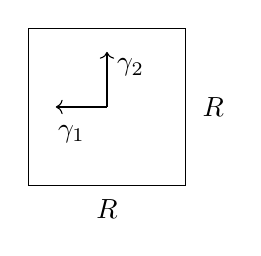
\begin{tikzpicture}
\draw (0,0)--(2,0)--(2,2)--(0,2)--(0,0);
\draw[->] (1,1)--(0.35,1);
\draw[->] (1,1)--(1,1.7);
\node at (0.55,0.65) {$\gamma_1$};
\node at (1.3,1.5) {$\gamma_2$};
\node at (2.35,1) {$R$};
\node at (1,-0.3) {$R$};
\end{tikzpicture}
\end{adjustbox}
\end{center}
\begin{equation*}
Z=\sum e^{-\beta\sum_{x',x''}H(x',x'')},\qquad\underline{Z=\operatorname{tr}A^R}.
\end{equation*}
$A^R$ --- матр. перех. от слоя к слою.
\underline{(2-мерная зад. Онзагера).}
\underline{Онзагер выч. все соб. значения этой матрицы:}
Здесь помогают антикомм. переменные: есть такие антикомм. матр. $A_i,A_j$, такие что
\begin{equation*}
A=e^{\sum c_{ij}A_i A_j}
\end{equation*}
и интегралы считаются.
[Справа, с двойной чертой:] см. \underline{Хуанг} «\underline{Стат. мех.}»
\underline{Либ} аналог. считал энтропию квадр. льда.
[Разделительная линия; далее лист пуст.]
\SourcePage{GELFAND-P000651}{unlabelled}
\underline{29/III-76. Сем. Гельфанда.}
\underline{Кричевер.} Задача решить ур-е $[L_1,L_2]=0$.
Если $\operatorname{ord}L_1$ и $\operatorname{ord}L_2$ вз. пр. --- ответ: кривая и расслоение (1-мерное).
Порядки не вз. просты --- возникают многомерные пучки.
Напр. 4-ый и 6-ый пор. не сделано. Свед. к 2-мерным расслоениям.
\begin{equation*}
\left.\begin{aligned}L_1y&=E_1y\\L_2y&=E_2y\end{aligned}\right\}\quad P(E_1,E_2)=0\quad\text{кривая}.
\end{equation*}
\Incomplete{GELFAND-P000651}{cancel-bundle}{Замаранный фрагмент под скобкой не восстановлен.}
Совм. решение --- 2-мерн. рассл. над кривой.
Вз. просты --- базис 1-мерный (из асимптотики).
$(m,n)=1\Rightarrow$ общ. соб. ф-й равно $n$ (и соб. знач. различны).
$E_1$ опр. по $E$.
$y$ однознач. опр. ф-я на рим. пов.
Обратная зад. по расслоению построить коммут. дифф. оп. --- не сделано.
\underline{Дринфельд.} $d=(m,n)\Rightarrow$ зад. пары комм. оп. $\longleftrightarrow$ зад. $(d-1)$ произв. ф-и.
\begin{equation*}B^{-1}LB\end{equation*}
разрешим --- ост. 1 произв. ф-я: старший коэфф.
4 и 6 пор. --- если в квадр. и кубик --- уже 2 произв. ф-и.
\underline{Шнирельман.} $M$ --- $n$-мерное рим. комп. аналит. многообразие.
$\Delta$ --- оп. Лапласа на $M$.
\begin{equation*}\Delta u_k+\lambda_k^2u_k=0.\qquad(1)\end{equation*}
[Определение $\Delta$; справа кружок с точкой в центре; за кружком справа текст «сф. рад. $\tau$»: ]
\begin{center}\begin{adjustbox}{max width=\linewidth}
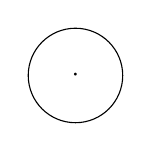
\begin{tikzpicture}
\draw (0,0) circle (0.6);
\node at (0,0) {$\cdot$};
\end{tikzpicture}
\end{adjustbox}\end{center}
\begin{equation*}
\frac{\text{ср. по сфере рад. }\tau-\text{зн. в центре}}{\tau^2}\longrightarrow\Delta f(x).
\end{equation*}
Рост с ростом $k$: $\lambda_k\sim c k^{1/n}$. \Incomplete{GELFAND-P000651}{cancel-square}{Зачёркнуто: a…; закрытый остаток не восстановлен.}
Пусть $a>0$. Как распр. $a\lambda_k\bmod 2\pi$ (часто есть арифм. прогрессии).
[На правом поле, с чертой сверху:] подпослед.
\underline{Тор.}
\begin{center}\begin{adjustbox}{max width=\linewidth}
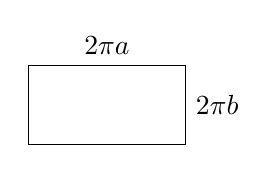
\begin{tikzpicture}
\draw (0,0)--(2,0)--(2,1)--(0,1)--(0,0);
\node at (1,1.25) {$2\pi a$};\node at (2.4,0.5) {$2\pi b$};
\end{tikzpicture}
\end{adjustbox}\end{center}
\begin{equation*}\Delta u=\lambda^2u.\end{equation*}
$\sin\alpha x\sin\beta y$ \Incomplete{GELFAND-P000651}{cancel-sine}{Зачёркнуто: cos…; остальное не восстановлено.} или $\cos\alpha x\sin\beta y$ и т.д.
\begin{equation*}\lambda^2=\frac{n^2}{a^2}+\frac{m^2}{b^2},\qquad\lambda=\sqrt{\frac{n^2}{a^2}+\frac{m^2}{b^2}}.\end{equation*}
Серии --- при разных $n$ и $m$ (при фиксир.).
Какие 2 номера --- неясно.
Теор. об 1-м пер. $-y''+u(x)y=\lambda y\Rightarrow$ на отрезке [горизонтальная черта с двумя концевыми черточками].
\begin{equation*}\sum_{i=0}^{n-1}c_i y_i\end{equation*}
имеет $\leq n$ нулей $\Rightarrow$ ведёт себя как пол. 1-й степ.
Отсюда 2 пер. многочлен от $n$ перем.
Наименьш. --- всюду положит.
1-я --- как лин. ф-и; далее --- кривая 2-го пор. --- следить за лин. комбин.
\SourceFigure{GELFAND-P000651}{oval-chords}{Два овала рядом; внутри каждого по наклонной кривой линии. Слева кривая идёт снизу слева вверх вправо и касается верхней правой границы, справа кривая --- от верхней левой границы вниз вправо с внутренним концом.}
\underline{Рэлей} теория звука (2 тома).
\underline{Арнольд.} Перенести теор. Харнака о числе овалов (у лин. комб. неизвестно).
[Справа, с двойной чертой; знак $\leq$ приписан перед «на»:] У $n$-й соб. ф-и нули делят обл. $\leq$ на $n$ частей.
\SourcePage{GELFAND-P000652}{unlabelled}
Рассмотрим
\begin{equation*}
\Phi(\lambda,a)=\lim_{\varepsilon\to0}\varepsilon\left(
\sum\delta((\lambda-a\lambda_k)\bmod2\pi)e^{-\varepsilon\lambda_k}
-\sum_k\frac{e^{-\varepsilon\lambda_k}}{2\pi}\right).
\end{equation*}
\begin{equation*}\mu_k=a\lambda_k\bmod2\pi.\end{equation*}
$\text{\Unclear{GELFAND-P000652}{distribution-letter}{$\mu\;?$}}$ --- распр. на окр.
\begin{equation*}
\Phi(\mu,a)=\lim_{\varepsilon\to0}\varepsilon\left(
\sum_{k=1}^{\infty}\delta(\mu-\mu_k)e^{-\varepsilon\lambda_k}
-\sum e^{-\varepsilon\lambda_k}/2\pi\right).
\end{equation*}
[Стрелка к вычитаемому члену:] вычесть, чтобы ср. знач. было $0$. постоянная.
$\Phi^\varepsilon(\mu,a)$ --- допред. выражение.
\underline{Теорема.} Пусть $\gamma_1,\gamma_2,\ldots$ --- замкнутые геодезич. на $M$,
$\ell(\gamma_1),\ell(\gamma_2),\ldots$ --- их длины.
Пусть \Unclear{GELFAND-P000652}{nondegenerate-abbreviation}{невд.?} расш. \Unclear{GELFAND-P000652}{dispersion-abbreviation}{диспр.?} обр., длины все разл. и несоизмеримы. (общее полож.).
\begin{equation*}
\Phi(\mu,a)\left\{\begin{aligned}
&=0\quad\text{если }a\ne\frac pq\ell(\gamma_j),\\
&\ne0\quad\text{[зачёркнуто]}\quad\text{если }a=\frac pq\ell(\gamma_j).
\end{aligned}\right.
\qquad(p,q\in\mathbb Z)
\end{equation*}
\Incomplete{GELFAND-P000652}{cancel-if}{Зачёркнутое слово перед вторым «если» неразборчиво.}
[На левом поле:] \SourceFigure{GELFAND-P000652}{geodesic-loop}{Замкнутая овальная кривая с подписью $\gamma_j$ справа; слева на контуре толстый направленный вверх знак, у верхнего левого участка наклонная стрелка вправо вверх. Наложение толстого левого знака не позволяет разделить все штрихи.}
рассм. геодезич. поток. ($\in SM$).
$S$ --- площ.; трансверс. замкн. геод. (разм. $2n-2$).
отобр. последования $\Psi:S\to S$.
$S\cap\gamma_j$ --- неподв. точка.
\begin{equation*}
d\Psi\big|_{S\cap\gamma_j}=\mathcal M\quad\text{--- опер. монодромии}\quad\text{(\underline{матр. монодромии})}.
\end{equation*}
Это преобр. \underline{симплектично}, т.к. поток гамильтонов.
Соб. числа расп. на пары и четверки.
\SourceFigure{GELFAND-P000652}{eigenvalue-drawings}{Четыре рисунка с горизонтальной и вертикальной осями и окружностями. 1) Два креста на правой части окружности: сверху $e^{i\alpha}$, снизу $e^{-i\alpha}$. 2) На положительной горизонтальной полуоси внутренний крест с подписью $\lambda$, внешний с подписью $1/\lambda$ снизу и $e^{\alpha_2}$ сверху. 3) На отрицательной полуоси внутренний крест без уверенно читаемой подписи; внешний крест подписан $-e^{\alpha_3}$. После 3) двойная вертикальная черта. Четвёртый рисунок без номера: два креста справа внутри окружности, к верхнему тонкая наклонная линия; два внешних креста справа, у верхнего подпись $e^{\alpha_4}$. Точные касания пересечений и контуров остаются в оригинале.}
[Справа от четвёртой схемы:] --- эти только в 3-мерн. пр-ве.
\underline{Рассм. коэфф. Фурье:}
\begin{equation*}
\Phi_n(a)=\int_0^{2\pi}\Phi(\mu,a)e^{-i\mu n}d\mu.
\end{equation*}
\begin{align*}
1)\quad\Phi_n(a)&=\frac c{\sin\dfrac{n\alpha_1}2},\\
2)\quad\Phi_n(a)&=\frac c{\operatorname{sh}\dfrac{n\alpha_2}2},\\
3)\quad\Phi_n(a)&=(-1)^n\frac c{\operatorname{sh}\dfrac{n\alpha}2}.
\end{align*}
$c$ зависит от размерности.
[Длинная охватывающая линия от формул слева к следующему справа.]
$1)$ $\alpha_1$ можно прибл. рацион. \Incomplete{GELFAND-P000652}{approximation-parenthesis}{[В скобках короткая письменная группа; последний знак похож на $\delta$, остальные знаки не восстановлены.]} $\Rightarrow$
\begin{equation*}
\text{A)}\quad\Phi(\mu,a)=\sum_{n=0}^{\infty}\delta\left(\mu-\left(n+\frac12\right)\alpha-\frac1{2\pi}\right).
\end{equation*}
(точно в рег. смысле
\begin{equation*}
\Phi(\mu,a)=\lim_{\varepsilon\to0}\sum_{n=0}^{\infty}\delta\left(\mu-\left(n+\frac12\right)\alpha e^{-n\varepsilon}-\frac1{2\pi}\right).
\end{equation*}
[На нижнем левом поле, подчеркнуто:] \underline{2 квант. числа} --- 2 индекса.
[На нижнем левом поле:] [Густой A-подобный знак.] Беск. число ар. прогрессий.


\SourcePage{GELFAND-P000653}{unlabelled}
2)
\begin{gather*}
\Phi(\mu,a)=c\sum_{m,n=-\infty}^{\infty}
\left(\frac{1}{\mu-n2\pi-(m+\frac12)i}
+\frac{1}{n2\pi+(m+\frac12)i\,[?]}\right)
=c\int_0^\mu\wp(\xi)\,d\xi,\\
\wp\text{ — ф-я Вейерштрасса.}
\end{gather*}
\Unclear{GELFAND-P000653}{period-end}{После $i$ во втором знаменателе дополнительный перечёркнутый знак: $\tau$? или $z$?}
\begin{center}
\begin{adjustbox}{max width=\linewidth}
\begin{tikzpicture}[x=0.8cm,y=0.8cm]
\draw (-1.2,0)--(1.5,0);
\draw (0,-0.9)--(0,1.2);
\node at (0,0.65) {$\times$}; \node at (1.2,0.65) {$\times$};
\node at (0,-0.65) {$\times$}; \node at (1.2,-0.65) {$\times$};
\node[right] at (1.8,-0.15) {$\leftarrow$ полюса};
\end{tikzpicture}
\end{adjustbox}
\end{center}
\SourceFigure{GELFAND-P000653}{curve-figure}{Слева под схемой полюсов: оси со стрелками вверх и вправо; кривая идёт от отмеченной крестом точки на горизонтальной оси вниз к минимуму на нижней горизонтали, затем вверх через начало координат к максимуму и вниз к правой отмеченной крестом точке. Нижняя горизонталь продолжается вправо после разрыва; под её левым отрезком густой неразобранный знак.}

Рассм. ф-я $f(z)=\sum_{k=1}^{\infty}e^{i\lambda k z}$.

Аналит. продолжается вниз с пр. полюсами.

[Справа рисунок: горизонтальная линия, над нею наклонная штриховка; четыре креста на линии; стрелка снизу к правому кресту с подписью
\Unclear{GELFAND-P000653}{pole-order}{$\ell(\gamma_j)$ или $\ell(\delta_j)$}.]

Фунд. реш. волн. ур-я. Продолже.

Вычеты в \Unclear{GELFAND-P000653}{pole-order}{$\ell(\gamma_j)$, $2\ell(\gamma_j)$, $\ldots$; $\gamma$ или $\delta$, как в подписи рисунка} —
\Unclear{GELFAND-P000653}{fourier-overwrite}{коэфф. / коэф.; буквы наведены друг на друга}
Фурье, и т. д.

\SourcePage{GELFAND-P000654}{unlabelled}
\underline{5/IV-76. Сем. Гельфанда. Поляков.}

Действие
\begin{gather*}
\left\{\begin{aligned}
S&=\frac{1}{4e^2}\operatorname{tr}\int A_{\mu\nu}^{2}\,d^4x\\
F_{\mu\nu}&=\partial_\mu A_\nu-\partial_\nu A_\mu+[A_\mu,A_\nu]
\end{aligned}\right.\\
A_\mu^+=-A_\mu,
\end{gather*}
$A_\mu$ — косоэрм. матр. $2\times2$, зав. ф-ей на $\mathbb R^4$.
[Под $A_\mu$ приписано: $\mu=0,1,2,3$.]

$A_\mu$ — поле; $S$ — ф-л от поля.

Классич. ур-я движ. — стационарность $S$.

Для чисел $A_\mu$ — эл.-магн. поле.

Аналог для дискр. $x$ и $t$.
[Подчёркнуто волнистой чертой.]

[Слева квадратная решётка: четыре примерно горизонтальные и четыре вертикальные линии.]
$x=(t,\vec x)$.
\begin{gather*}
S=\frac{1}{4e_0^2}\sum_{\vec x}\chi\left(
B_{\vec x,\mu}\,B_{\vec x+\vec a_\mu,\nu}\,
B_{\vec x+\vec a_\nu,\mu}^{-1}\,B_{\vec x,\nu}^{-1}\right).\\
a_\mu\text{ — репер,}\qquad B_{\vec x,\mu}\in SU(2).
\end{gather*}
$\chi$ — любой характер
( [зачёркнуто слово]
\Incomplete{GELFAND-P000654}{cancelled-character}{Зачёркнутое слово перед «ф-я» не разобрано.}
ф-я, пост. на классах сопр. элем. — например, след).
\begin{gather*}
Z=\int\prod_{\vec x,\mu}dB_{\vec x,\mu}\ e^{-S(B)}.
\end{gather*}
$12n$ незав. переменных ($n$ — число точек решётки; в $\forall$ — 4 матрицы).

$B_{\vec x,\mu}$ — незав. пер. $\Rightarrow$
$dB_{\vec x,\mu}$ — \underline{инв. мера}
($4n$ интегралов по инв. мерам).
\begin{gather*}
t\to it\quad\Rightarrow\quad e^{iS}\to e^{-S}.
\end{gather*}
В непр. случае — функц. интеграл.
[Отделено волнистой чертой.]

Коррел. ф-и
[далее ряд точек].

\SourcePage{GELFAND-P000655}{unlabelled}
\underline{12/IV-76. Сем. Гельфанда.}

\underline{Фукс.} Применение выч. машин в теор. математике.
[Подчёркнуто волнистой чертой.]

Выч. когом. алгебры форм. бездиверг. вект. полей
Есть $\mathbb R^n$. Рассмотрим $(\mathbb R^n)'$ и полиномы
\begin{gather*}
p(\xi_1,\ldots,\xi_q;\eta_1,\ldots,\eta_q),\qquad
\xi_i\in\mathbb R^n,\quad\eta_i\in(\mathbb R^n)'.
\end{gather*}
Они облад. св-вом

а) если пару $\xi_i,\eta_i$ поставить на место $\xi_j,\eta_j$, то полином меняет знак.

$dP=P_1$ зад. ф-лой
\begin{align*}
P_1(\xi_1,\ldots,\xi_{q+1},\eta_1,\ldots,\eta_{q+1})
&=\sum_{i<j}(-1)^{i+j-1}[(\xi_i,\eta_j)-(\xi_j,\eta_i)]\\
&\quad p(\xi_i+\xi_j,\xi_1,\ldots,\widehat\xi_i,\ldots,\widehat\xi_j,\ldots,\xi_{q+1},\\
&\qquad\eta_i+\eta_j,\eta_1,\ldots,\widehat\eta_i,\ldots,\widehat\eta_j,\ldots,\eta_{q+1}).
\end{align*}
\underline{Задача:} найти когомологии этого комплекса (до сих пор не сделано).

Выч. машина помогла найти нетрив. циклы.

Рассм. линейные по $\eta$: тогда это комплекс когом. алгебры $W_n$.

Не сделано даже для $n=1$.

Все получ. рез. относятся к этому случаю.

Комплекс = сумма большого числа кон.-мерных.

Суммар. степень по $\xi$: $m_1+q$,
по $\eta$: $m_2+q$ [справа: \underline{подкомплекс} $K_{m_1,m_2}$].

($q$ меняется.)

мн-ки от $\xi_1,\ldots,\xi_q,\eta_1,\ldots,\eta_q$.
[Подчёркнуто и выделено правой чертой.]

Каждый из них конечномерен.

$m_1\ne m_2\Rightarrow$ он ацикличен.

В действит. $\sum$ гомол. счётн. числа подкомпл.
\begin{gather*}
H(K)=\bigoplus_m H(K_{m,m}).
\end{gather*}
(пока $n$ произвольно.)

\underline{$n=1$.}

$m=1,2,3$ — ацикличны.

\underline{$m=4$} нетрив. в разм. \underline{$7$ и $10$} — считали на машине
(Гельфанд, Фукс, Камынин).

\underline{$m=5$} — «переполнение рабочего поля $N=2$».

\underline{Эйлерова хар-ка} не зав. от дифференциала.

\underline{Першик} (асп. Ботта) досчит. до \underline{$m=35$}.
\begin{gather*}
K_{m,m}\supset K'_{m,m}\qquad
H(K_{m,m})=H(K'_{m,m})\otimes H(S^3).\\
\chi_m^*\text{ — ?}\qquad(\text{для }K'_{m,m}).
\end{gather*}
\underline{Першик нашёл} производ. ф. для $\chi_m$.

\Unclear{GELFAND-P000655}{bottom-word-full}{Интересно:; средние буквы наведены / исправлены}
док., что при сколь угодно больших $m$ есть $\chi_m\ne0$.
\begin{gather*}
\begin{aligned}
&\frac12(1-t^{-1}x^{-1})(1-t^{-1}x)\\
&\qquad(1-x^{-2})\qquad(1-x^2)\\
&(1-tx^{-3})(1-tx^{-1})(1-tx)(1-tx^3)\\
&\ldots
\end{aligned}
\end{gather*}

\SourcePage{GELFAND-P000656}{unlabelled}
\begin{gather*}
(1-t^\ell x^{-\ell-2})(1-t^{[2?]}x^{-\ell})\ldots(1-t^\ell x^{\ell+2}).
\end{gather*}
\Unclear{GELFAND-P000656}{middle-t-power}{Средний показатель при $t$: $2$? или $\ell$?; густо наведённый знак.}
Берём произведение всех. Выбрасываем всё, что сод. $x$. Тогда получится
\begin{gather*}
\sum\chi_m t^{2m}=t^{-2}+2-t^8-t^{14}-t^{22}+\ldots+10t^{70}+\ldots
\end{gather*}
Написали разл. до $t^{70}$.

(Доказано сущ. $\ge57$ нетрив. [вставлено сверху: кл.] когомологий.)

\underline{Бухштабер} о раб. Адамса о раб. Бухштабера.

$X$ — топ. пр-во. Рассм. $X\times X\to X$ для группы. $\Rightarrow$

[Слева, со стрелкой к «Рассм.»: Если $X$ — наст. группа, то]
\begin{gather*}
C(X\times X)\leftarrow C(X)\text{ — структ. коалгебры.}
\end{gather*}
Грубо:
\begin{gather*}
M(f(x\cdot y))\leftarrow f(x)\\
(\text{мат. ожидание значений}).
\end{gather*}
[Разделитель: два коротких штриха и точка.]

\underline{С. П. Новиков. Общая теор. относительности.}

Читать: Ландау и Лифшиц (вместе с рим. геометрией) — Теор. поля.

$(t,\vec x)$ — пр-во событий; $(t,\vec x)\to(x^0,\vec x)$, $x^0=ct$.
\begin{gather*}
ds^2=g_{ij}\,dx^i\,dx^j,\qquad
g_{ij}=\begin{pmatrix}1&&&0\\&-1&&\\&&-1&\\0&&&-1\end{pmatrix}.
\end{gather*}
Соб. время — длина кривой.

Пусть $M^4$; зад. $g_{ij}$. И — сист. коорд. $x^0,x^1,x^2,x^3$.

\underline{Эйнштейн:} метрика назв. гравит. полем (1913) (+ Гроссман).

\underline{Ур-е Эйнштейна} — незав. Эйнштейн и Гильберт (1916).
\begin{gather*}
R_{ij}-\frac12Rg_{ij}=\frac{8\pi k}{c^4}T_{ij}.
\end{gather*}
[Формула выделена нижней скобой.]

Здесь $R_{j\ell}=\sum_i R^i_{ji\ell}$ — тензор Риччи.

[Справа:] $(R^i_j)_{k\ell}$ — 2-форма (кососимм. по $k,\ell$) со знач. в алг. Ли гр. $O(n)$.

$T_{ij}$ — тенз. эн.-имп. материи (внешняя масса).
[Справа:] $T_{ij}$ ответ. за всё, кроме гравит. поля.
\begin{gather*}
R=\sum_{j,\ell}g^{j\ell}R_{j\ell}.
\end{gather*}
В люб. размерности
\begin{gather*}
R_{ij}-\frac12Rg_{ij}=T_{ij}.
\end{gather*}
[Формула выделена нижней скобой и подчёркнута волнистой чертой.]

Пусть физ. велич. опред. лагранжианом $L$.
\begin{gather*}
S=\int L(q,g_{ij})\sqrt g\,d^4x.
\end{gather*}
[Под $\sqrt g\,d^4x$ скоба:] $d\sigma$ — инв. эл. объёма.

Тогда
\begin{gather*}
\sqrt g\,T_{ij}=\frac{\delta S}{\delta g_{ij}}.
\end{gather*}
\underline{Эл.-магн.}
\begin{gather*}
L_{\text{элм.}}=F_{\mu\nu}F^{\mu\nu},\quad
\text{где}\quad F_{\mu\nu}dx^\nu\wedge dx^\mu=d(\vec A).
\end{gather*}
[Стрелка от «вх. метрика.» к $F^{\mu\nu}$.]

\underline{Нет сил:} $\Rightarrow\displaystyle\frac{\delta S}{\delta g^{ij}}=0$.
\begin{gather*}
S=\int R\sqrt g\,d^4x.
\end{gather*}

\SourcePage{GELFAND-P000657}{unlabelled}
\underline{Ур. Эйнштейна:} в грав. поле нет эн.-имп., кроме той, к-рая в других видах энергии.

\underline{Г.} Квантуется ли? Если да, то нет метрики (геом. структуры м-ва).

\underline{Н.} Но это влияет лишь на $10^{-33}$ см (а ядерные взаимод. на $10^{-23}$ см).

Пока имеет смысл: пр-во — сохр. ур-е Эйнштейна.

Квант. мех. огранич. лишь временами $10^{-43}$ сек.
\begin{gather*}
T_{00}\text{ — плотн. энергии}=\varepsilon>0.
\end{gather*}
[Перед следующим словом зачёркнут заголовок.]
\Incomplete{GELFAND-P000657}{cancelled-heading}{Зачёркнутый заголовок не разобран; видимы отдельные буквы, возможно начало «Выч».}
\underline{Задачи}
[Подчёркнуто волнистой чертой.]

1) \underline{приближ. сплошной среды}: гидродин. вид с зак. Паскаля
\begin{gather*}
T_{ij}=(p+\varepsilon)u_i u_j-pg_{ij}.
\end{gather*}
[Справа:] ($p$ — давл., $\varepsilon$ — плотн. энергии

$\varepsilon,p,\vec u$ — ф-и точки.
\begin{gather*}
\varepsilon=\varepsilon(p)\text{ — задана}\qquad\text{или}\quad p=p(\varepsilon).
\end{gather*}
\underline{Задача:} найти $(M^4,g_{ij})$. Пылевидная жидкость $p=0$.

или $p=\dfrac{\varepsilon}{3}$ — ультрарелятив. жидкость (свет

Гидродин. — $g_{ij}$ — обычн. коор.
\begin{gather*}
\sum_k\nabla_k T_i^k=0\quad\Rightarrow\quad\text{законы гидродин.}
\end{gather*}
[Левая часть подчёркнута волнистой чертой.]

Поле точечн. массы
\begin{gather*}
R_{ij}-\frac12Rg_{ij}=\delta_{[ij?]}(r,t).
\end{gather*}
\Unclear{GELFAND-P000657}{stress-index}{Нижний индекс при $\delta$: $ij$?; густо наведённые знаки.}
гр. симм. $SO(3)$ — \underline{реш. Шварцшильда}. Впервые $M^4$ указ. в 1960 г.
Крускалом. Сферич. коорд. опис. одну карту (и не всё мн-зие).

$r$ в прив. коорд. им. \underline{сёдла} (гравит. радиусы).

\Unclear{GELFAND-P000657}{novikov-abbreviation}{С. с. д. / С. с. о.} раз \underline{Новиков}.

\underline{19/IV-76. Сем. Гельфанда.}
[Название семинара подчёркнуто волнистой чертой.]

\underline{Проблема Серра.} Будет ли всякий $\mathbb C[x_1,\ldots,x_n]$ — модуль свободен?
[Над $\mathbb C[x_1,\ldots,x_n]$ — модуль, в обведённой выноске со стрелкой: проективный.]

[Разделитель: два коротких горизонтальных штриха с кружком между ними.]

\underline{Гельфанд и замечания Васерштейна}
\begin{gather*}
a_1,\ldots,a_k\in\mathbb C[x_1,\ldots,x_n]=A.
\end{gather*}
наз. унимодулярной, если $\exists p_1,\ldots,p_k:\ \sum p_i a_i=1$.

Сущ. ли матрица с элем. из $A$, и с \underline{$\det=1$}
\begin{gather*}
\begin{pmatrix}a_{11}&\ldots&a_{1k}\\a_{k1}&\ldots&a_{kk}\end{pmatrix},
\end{gather*}
\Unclear{GELFAND-P000657}{matrix-index-corrections}{Индексы $a_{11},a_{1k},a_{k1}$ наведены или исправлены; прежние знаки не установлены.}

и с 1-й строчкой [зачёркнуто $a_{11},\ldots,a_{1k}$] $a_1,\ldots,a_k$?

\underline{Дринфельд} об этом же.

$B$ — кольцо
\begin{gather*}
f=\begin{pmatrix}f_1\\\vdots\\f_n\end{pmatrix}
\text{ — унимод. столбец в }B[x]
\end{gather*}
($x$ — одна пер.)

\underline{старш. коэфф. $f_1=1$} Тогда $f(x)\sim f(0)$
(перев. невыр. матрицей над $B[x]$).

Осн. средство — \underline{результант}:
\begin{gather*}
\prod(\xi_i-\eta_k)
\end{gather*}
[Справа:] $\xi_i,\eta_k$ — корни 2-х мног. 1-й пер.

\SourcePage{GELFAND-P000658}{unlabelled}
\underline{Осн. лемма.} Пусть $c=\operatorname{Res}(f_1,f_2)$. Тогда если $f$ — любой столбец, то
\begin{gather*}
f(Y_1+cY_2)\ [\sim?]\ f(Y_1)
\quad\text{над }B[Y_1,Y_2].
\end{gather*}
\Unclear{GELFAND-P000658}{lemma-equivalence}{Между двумя столбцами знак $\sim$?; наведён несколькими волнистыми штрихами.}
\underline{Док.:} явной конструкцией (\underline{Суслин})

\underline{Надо:} $c=1$ и положить $Y_2=-Y_1$.

\underline{Редукция к этой лемме.}

Замена пер. сводит к случаю, когда 1 из старш. коэфф. 1.

По очереди убираем все перем.

\underline{С. П. Новиков.}

$M^n,g_{ij}$, сигн. $(1,-1,-1,-1)$
\begin{gather*}
R_{ij}-\frac12Rg_{ij}=T_{ij}.
\end{gather*}
[Справа, за двойной вертикальной чертой:]
\underline{Сф. симм. зад.}: до конца в 1960 Крускал.
[«до конца» и нижняя строка подчёркнуты волнистыми чертами.]

Физ. пост. задачи — гипотезы на $T_{ij}$.

Сплошн. среда
\begin{gather*}
T_{ij}=(p+\varepsilon)u_i u_j-pg_{ij},\quad\text{где }p=p(\varepsilon),\\
\vec u=(u_0,u_1,u_2,u_3);\qquad 1=\langle u,u\rangle.
\end{gather*}
Пыль: $p=0$. Скор. звука:
\begin{gather*}
c_{\text{зв}}^2=\frac{\partial p}{\partial\varepsilon}\ge0,\\
c_{\text{зв}}^2\le c^2=1.
\end{gather*}
Ур-ий не хватает. Но: есть калибр. преобр.

\underline{Гильберт} написал ур-я, но отказался как от неправильных.

Есть метрика \underline{Гёделя} (того самого) с замкнутой времениподобной
линией (мнимая?).



\end{document}
